\documentclass[lang=cn,12pt,chinesefont=founder]{elegantbook}

\title{高中数学基础一本通}
\author{Midnight Forever (永远是深夜有多好)}
\date{\today}
\version{20250715}
\extrainfo{请尊重作者个人的编写编辑的知识成果.}

\definecolor{customcolor}{RGB}{255,20,147}
\colorlet{coverlinecolor}{customcolor}
\logo{image/logo.png}
\cover{image/cover.png}
\setcounter{tocdepth}{3}

\usepackage{tikz}                  
\usetikzlibrary{trees, arrows.meta, patterns} 
\usetikzlibrary{positioning}
\usepackage{booktabs}   
\usepackage{tabularx}  
\usepackage{float}     
\usepackage{amsmath}  
\usepackage{amsfonts}  
\usepackage{amssymb}    
\usepackage{fancyhdr}   
\usepackage{xcolor}
\usepackage{lettrine}  


\newcommand{\qed}{\hfill $\Box$}
\newcommand{\makechapteropener}[4]{
	\newpage
	\thispagestyle{empty} 
	
	\vspace*{\fill} 
	
	\begin{center}
		{\songti \Huge 第#1章}
		\vspace{2cm} 
		{\heiti \huge #2}
	\end{center}
	
	\vfill 
	
	\begin{center}
		\begin{minipage}{0.75\textwidth} 
			\centering 
			{\kaishu \large “#3”} 
			\par\vspace{1em} 
			\begin{flushright} 
				--- #4
			\end{flushright}
		\end{minipage}
	\end{center}
	
	\vspace*{2cm}
	\cleardoublepage 
}


\begin{document}
	
	\maketitle
	
\begin{titlepage}
	\begin{center} 
		
		\vspace*{3cm} 
		
		% --- 标题 ---
		{\Huge\bfseries\kaishu 高中数学基础一本通\par} 
		
		\vspace{5cm}
		
		% --- 作者 ---
		{\LARGE 作者\par}
		\vspace{0.7cm}
		{\Large Midnight Forever (永远是深夜有多好)\par}
		
		\vfill 
		
		{\large
			版本号:20250715 \par
			\vspace{0.2cm}
			日期:\today \par
		}
		
		\vspace{2cm}
		
		{\itshape 请尊重作者个人的编写编辑的知识成果。} 
		
	\end{center}
\end{titlepage}
	

	\frontmatter
	\tableofcontents
	
	\mainmatter 

	\pagestyle{fancy}

	\fancyhf{}
	
	\fancyhead[LE]{\leftmark}
	\fancyhead[RO]{\rightmark}
	
	\renewcommand{\headrulewidth}{0.4pt}
	
	
	\fancyfoot[C]{编者:Midnight Forever (永远是深夜有多好)}
	\fancyfoot[RO,LE]{\thepage}

	\chapter*{写在前面}
	\thispagestyle{fancy} 

	\lettrine{嗨}{,同学},你好.我是 Midnight Forever,一名和你一样,在题海中沉浮过的高考考生.这本书的诞生,源于在高考后,我突然奇想,能不能把我零散的笔记、错题和感悟整理成一本所谓的学霸笔记,或许还能赚点零花钱.然而,当我真正开始动手整理时,我翻阅了市面上许多资料,包括一数的“高考数学一本通”与我校老师们辛苦编撰的回归教材系列.我渐渐发现了许多优秀资料的闪光点,也看到了它们可以被改进、被超越的地方.
	
	于是我继续想,我否自己写本更系统、更优雅、更贴近备考真实需求的数学复习资料?于是这本书便产生了.相较于市面上琳琅满目的复习资料,这本书倾注了我对数学之美的理解和对学习效率的执着追求,并力求在以下几个方面做到极致:
	
	\begin{enumerate}
		\item \textbf{排版之美}
		我相信,一份赏心悦目的学习资料,能从心理上点燃各位的学习热情.本书采用\LaTeX{}排版,精心设计了字体(本书主要使用宋体,笔记和解析等部分使用楷体,粗体和重点使用黑体,统一分明)、版式与色彩,力求让每一个公式、每一幅图、每一段文字都清晰、优雅、和谐.
		
		\item \textbf{保姆级解析}
		受到一数教辅“蓝字”引导式解析的启发,我再此基础上,采取了一套更系统,更有条理的解析布局.有时我想你对着答案解析,每一步都看得懂,但合上书,自己却依然无从下手?这是因为许多答案只告诉你是什么,却没告诉你为什么这么想.本书的解析,也将遵循“\textbf{思路分析} $\to$ \textbf{核心技巧} $\to$ \textbf{解题步骤} $\to$ \textbf{归纳总结}”的模式,更重要的是,和你分享每一步背后的思考过程,让你真正建立起“我知道下一步要做什么”的解题逻辑流.本书的解析格式,是为了避免让你陷入“做到一半不知道自己要干嘛”,“不得不回头重新看去”的尴尬局面,减少乱试浪费的时间.
		
		\item \textbf{数形结合}
		笔者最讨厌的事之一就是解析答案说一大堆,结果一张图都没有. 不可否认这可能是解析在锻炼我们的画图能力,这本身也是一种学习的过程. 但是出于方便理解和本书的“优雅”哲学,我尽可能的配图了. 这一哲学将在解析几何与概率统计部分体现得淋漓尽致,在那里,我将使用图示帮助拆解概率统计的阅读理解题,并用图示将我们要介绍的解析几何知识与各种模型生动地体现出来.
		
		\item \textbf{聚焦基础,拒绝炫技.}
		高考数学,得基础者得天下.本书坚决摒弃各种偏难怪题和华而不实的“秒杀技巧”.我们只专注于那些占据了高考试卷绝大多数分值的核心基础知识、核心题型与核心思想方法.我们的目标是帮你夯实地基,让你在面对任何基础题和中档题时都能稳操胜券,为挑战更高难度的题目积蓄最强大的能量与自信.
	\end{enumerate}
	
	当然,作为一名仍在求学路上的学生,我的知识水平和视野终究有限,书中难免会出现疏忽与错漏.在此,我恳请各位同学和老师,在使用过程中若发现任何问题,能够不吝赐教,通过QQ(2454167821)与我联系.你们的每一条反馈,都将是这本书不断完善、走向完美的阶石.
	
	愿这本书,能成为你高三征途中一位温暖而有力的同伴.
	
	\vspace{2cm} 
	\begin{flushright}
		Midnight Forever (永远是深夜有多好) \\
		\today
	\end{flushright}
	
	
	\newpage
	\thispagestyle{empty}
	
	\begin{center}
		\vspace*{4cm} 
		
		\begin{tikzpicture}
			\node[font=\Huge\bfseries] at (0,0) {关于作者};
			\draw[thick, color=customcolor] (-3,-0.5) -- (3,-0.5);
		\end{tikzpicture}
		
		\vspace{2cm}
		
		\Large \textbf{Midnight Forever} \\
		\large (永远是深夜有多好)
		
		\vspace{1.5cm}
		
		\begin{minipage}{0.8\textwidth}
			\large
			2025届高考考生,来自某普通高中的一名文科生(政史地组合).
			
			\vspace{0.5cm}
			作为文科生,众所周知文科最能拉分的便是数学与英语两科,因此整个高中大部分时间我都投入于这两个科目,也取得了不错的成绩 .我也相信学习高中数学更是一种锻炼思维、欣赏理性的艺术的过程. 我今年在2025年高考新二卷中取得139分的成绩,在文科中我自认为也处于中上游水平了. 而且这段经历让我深刻体会到,扎实的基础和清晰的思维逻辑,远比盲目的题海战术更为重要.
			
			\vspace{0.5cm}
			编写此书,是希望将这份对数学的理解与热爱分享出去,帮助更多像我一样,并非天赋异禀,但愿意脚踏实地、探求甚解的同学. 希望能通过这份资料,让大家感受到数学的逻辑之美与解题的思维之乐.
			
			\vspace{0.5cm}
			感谢你的阅读,愿我们都能在数学的世界里,找到属于自己的那片星空.
		\end{minipage}
	\end{center}
	
	\newpage
	\thispagestyle{fancy} 
	
	\begin{center}
		\vspace*{4cm}
		
		\begin{tikzpicture}
			\node[font=\Huge\bfseries] at (0,0) {常见问题与解答};
			\draw[thick, color=customcolor] (-4.5,-0.5) -- (4.5,-0.5);
		\end{tikzpicture}
		
		\vspace{2cm}
	\end{center}

	{\large 
		
		\noindent 
		\textbf{Q: }完整的本书会包括哪些内容?
		\par\vspace{0.3cm} 
		\noindent
		\textbf{A: }将包括高中数学的所有内容.
		
		\par\vspace{1cm} 
		
		\noindent
		\textbf{Q: }本书是什么性质?参考书还是教科书?
		\par\vspace{0.3cm}
		\noindent
		\textbf{A: }笔者认为,参考书是你不需要从头读起,可以随时翻阅特定概念的工具书,它需要一定的知识储备;而教科书则逻辑紧密,需要从头学起,对预备知识要求不高.本书并非严格的其中一种,而是兼具两者之长.例如,在前面的章节中,你可能会看到“导数”的提前出现与应用,尽管它的系统讲解在后几章.高中数学各模块联系紧密,无法完全割裂.因此,我建议读者善于前后翻阅,体会作者在章节编排上的用心.
		
		\par\vspace{1cm}
		
		\noindent
		\textbf{Q: }本书是否免费?
		\par\vspace{0.3cm}
		\noindent
		\textbf{A: }并不.本书的制作,包括排版、编辑、绘图和校对等工作,均由我一人利用课余时间完成,投入了大量心血.如果您觉得本书对您有帮助,认可我的劳动与付出,可以花费几块钱购买完整版以支持我.当然,如果觉得编写得不尽如人意,市面上也有许多优秀的教辅可供选择,如一数的《必刷100讲》、新高掌等.
		
		\par\vspace{1cm}
		
		\noindent
		\textbf{Q: }为什么没在书里看见高考真题和模拟题?
		\par\vspace{0.3cm}
		\noindent
		\textbf{A: }因为还没加.得益于我在高三时所做的工作——系统地收集和分类了大量优质真题与模拟题,因此将其插入本书并不困难.真正的挑战在于,如何按照本书保姆级解析的风格,重写每一道题的解析.
		
		\par\vspace{1cm}
		
		\noindent
		\textbf{Q: }本书会包含“拉格朗日乘数法”、“奔驰定理”这类大招或二级结论吗?
		\par\vspace{0.3cm}
		\noindent
		\textbf{A: }会的,但会以星号(*)标记,表明其为拓展内容,并非人人必需.对于“奔驰定理”这类在特定地区(如浙江卷)较常出现,但在全国卷中几年下来几乎没考过的内容,本书也会收录,并加以注明.这些章节的加入,是出于知识的完整性和本书的“参考书”属性考虑.
		\par\medskip 
		关于“大招”和“二级结论”,尤其是在解析几何部分,我想特别说明一点.许多资料热衷于介绍各种技巧,但笔者认为,\textbf{对于绝大多数中等水平的同学而言,考场上有限的时间和巨大的压力,往往会让他们回归到最稳妥、最通用的方法,比如设点联立.(比如某位同学学了一堆技巧大招,最后在考场上还是设元联立...)}与其花费大量时间学习可能用不上、用不熟的技巧,不如将基础打得更牢.因此,本书在讲解解法时,会更侧重于两个层次:首先,清晰地讲授如何通过常规方法(如设元联立、求切线等)迅速拿到大部分基础分;其次,再探讨如何在此基础上进一步思考,向更高分迈进.我希望这种务实的编排思路,对读者有所帮助,且后来被证明是合理的.
		
	} 
		\makechapteropener
	{一} 
	{基础} 
	{将一个难题分解为若干个更小的、可解决的部分,是攻克它的第一步。} 
	{勒内·笛卡尔 (René Descartes)} 
	
	\chapter{基础}
	
	\lettrine{在}{正式踏上}高中数学的复习征途之前,我们需要进行一次彻底的“热身”与“装备检查”.本章并非全新的知识,而是对那些贯穿整个高中数学、须臾不可离的基础技能与核心思想的再强化,基础不稳,寸步难行.让我们开始吧.
	
\begin{introduction}[知识概括]
	\item \textbf{因式分解:} \label{intro:factor} 系统掌握提公因式、公式法、十字相乘法、分组分解法四大基本技巧,并学会高次多项式的猜根与综合除法.
	\item \textbf{一元二次方程根的分布:} \label{intro:roots_dist} 这是连接函数、方程、不等式的核心难点.关键在于掌握判别式、对称轴、端点函数值这“三大抓手”,将根的几何位置问题转化为代数不等式组问题.
	\item \textbf{核心计算与变形技巧:} \label{intro:techniques} 熟练运用配方法、换元法、待定系数法等“万金油”式的代数技巧,它们是化繁为简、解决复杂问题的钥匙.
\end{introduction}
	
	\section{因式分解核心技巧}
	
	因式分解是多项式乘法的逆运算,是将一个多项式化为若干个整式的乘积的形式.它是解方程、化简分式、研究函数性质的基础.掌握其方法,是代数运算能力的基石.
	
	\subsection{提公因式法}
	这是所有因式分解方法中最优先考虑的方法.其核心是找到多项式各项中都含有的公共的因式(可以是单项式,也可以是多项式),然后将其提取出来.
	\begin{exercise}
		分解因式:$3x(a-b) - 2y(b-a)$.
	\end{exercise}
	\begin{solution}
		观察到 $(b-a) = -(a-b)$,所以两项中含有公因式 $(a-b)$.
		\begin{align*}
			3x(a-b) - 2y(b-a) &= 3x(a-b) - 2y[-(a-b)] \\
			&= 3x(a-b) + 2y(a-b) \\
			&= (a-b)(3x+2y)
		\end{align*}
	\end{solution}
	\qed
	
	\subsection{公式法}
	熟练运用乘法公式的逆运算,是快速分解特定形式多项式的关键.
	\begin{itemize}
		\item \textbf{平方差公式}: $a^2-b^2=(a+b)(a-b)$
		\item \textbf{完全平方公式}: $a^2 \pm 2ab + b^2 = (a \pm b)^2$
		\item \textbf{立方和/差公式}: $a^3 \pm b^3 = (a \pm b)(a^2 \mp ab + b^2)$
	\end{itemize}
	\begin{exercise}
		分解因式:$x^4 - 16$.
	\end{exercise}
	\begin{solution}
		该式可看作 $(x^2)^2 - 4^2$,首先应用平方差公式.
		\begin{align*}
			x^4 - 16 &= (x^2)^2 - 4^2 \\
			&= (x^2-4)(x^2+4) \\
			&= (x-2)(x+2)(x^2+4)
		\end{align*}
		注意:分解务必彻底,$x^2-4$ 还可以继续分解.$x^2+4$ 在实数范围内不能再分解.
	\end{solution}
	\qed
	
	\subsection{十字相乘法}
	这是分解二次三项式 $ax^2+bx+c$ 的核心技巧.其本质是寻找两个数,使其和为一次项系数,积为常数项与二次项系数的乘积.
	\begin{exercise}
		分解因式:$6x^2 - 5x - 4$.
	\end{exercise}
	\begin{solution}
		我们将首项 $6x^2$ 分解为 $2x \cdot 3x$,将常数项 $-4$ 分解为 $1 \cdot (-4)$ 或 $-1 \cdot 4$ 等.通过尝试,我们发现:
		\begin{center}
			\begin{tikzpicture}
				\node at (0,0.5) {$2x$};
				\node at (0,-0.5) {$3x$};
				\node at (2,0.5) {$1$};
				\node at (2,-0.5) {$-4$};
				\draw (0.3,0.5) -- (1.7,-0.5);
				\draw (0.3,-0.5) -- (1.7,0.5);
				\node[right, blue] at (2.5, 0) {交叉乘积和: $(2x)(-4) + (3x)(1) = -8x+3x = -5x$};
			\end{tikzpicture}
		\end{center}
		交叉乘积之和等于一次项系数 $-5x$,所以分解成功.
		$6x^2 - 5x - 4 = (2x+1)(3x-4)$.
	\end{solution}
	\qed
	
	\subsection{分组分解法}
	对于四项或四项以上的多项式,如果不能直接提公因式或套公式,可以尝试将其合理分组,使组内能分解,进而使组与组之间产生新的公因式.
	\begin{itemize}
		\item \textbf{二二分组}: 例如 $am+an+bm+bn = (am+an)+(bm+bn)$.
		\item \textbf{三一分组}: 通常是三项构成完全平方式,再与剩下的一项构成平方差.
	\end{itemize}
	\begin{exercise}
		分解因式:$x^2 - 4y^2 + 2x + 1$.
	\end{exercise}
	\begin{solution}
		观察到 $x^2, 2x, 1$ 这三项可以构成完全平方式.
		\begin{align*}
			x^2 - 4y^2 + 2x + 1 &= (x^2 + 2x + 1) - 4y^2 \\
			&= (x+1)^2 - (2y)^2 \\
			&= [(x+1)-2y][(x+1)+2y] \\
			&= (x-2y+1)(x+2y+1)
		\end{align*}
	\end{solution}
	\qed
	
	\subsection{高次多项式猜根与综合除法}
	对于整系数高次多项式,如果它有有理根,那么这个根一定是“常数项的因数 / 最高次项系数的因数”的形式(有理根定理).这为我们“猜根”提供了方向.
	\begin{definition}[综合除法]
		当猜出一个根 $x=a$ 后,说明多项式必有因式 $(x-a)$.综合除法是快速计算多项式除以 $(x-a)$ 的商式的竖式算法.
	\end{definition}
	\begin{exercise}
		分解因式:$x^3 - 2x^2 - 5x + 6$.
	\end{exercise}
	\begin{solution}
		常数项为6,其因数有 $\pm 1, \pm 2, \pm 3, \pm 6$.最高次项系数为1.
		尝试将 $x=1$ 代入:$1-2-5+6=0$.成功!所以必有因式 $(x-1)$.
		用 $(x-1)$ 去除原多项式:
		\begin{center}
			\begin{tabular}{c|cccc}
				1 & 1 & -2 & -5 & 6 \\
				&   & 1  & -1 & -6 \\
				\hline
				& 1 & -1 & -6 & \textbf{0} \\
			\end{tabular}
		\end{center}
		商式为 $x^2-x-6$.所以 $x^3 - 2x^2 - 5x + 6 = (x-1)(x^2-x-6)$.
		对 $x^2-x-6$ 使用十字相乘法,得 $(x-3)(x+2)$.
		所以,最终分解结果为 $(x-1)(x-3)(x+2)$.
	\end{solution}
	\qed
	
	\section{一元二次方程根的分布}
	
	这是一个综合性极强的问题,深刻体现了数形结合思想.它探讨的是一元二次方程 $ax^2+bx+c=0 \ (a>0)$ 的两个实数根 $x_1, x_2$ 相对于某个给定值 $k$ 的位置关系.
	
	\begin{note}[核心思想:几何问题代数化]
		解决此类问题的根本,在于将“根的分布”这一\textbf{几何位置描述},通过二次函数 $y=ax^2+bx+c$ 的图像特征,转化为关于系数的\textbf{代数不等式组}.我们必须学会用代数语言去描述几何形态.
	\end{note}
	
	\begin{theorem}[古希腊掌管根分布的神]
		要精确地“定位”抛物线的根,我们通常需要从三个方面进行约束:
		\begin{enumerate}
			\item \textbf{判别式 $\Delta=b^2-4ac$}:它掌管着“\textbf{有没有根}”.$\Delta \ge 0$ 是方程有实根的前提,是所有讨论的基石.
			\item \textbf{对称轴 $x = -\frac{b}{2a}$}:它掌管着“\textbf{根的整体位置}”.对称轴在 $k$ 的左边还是右边,决定了两个根是“整体靠左”还是“整体靠右”.
			\item \textbf{端点函数值 $f(k)$}:它掌管着“\textbf{根与特定点的相对位置}”.$f(k)$ 的符号决定了点 $k$ 是在两根之间 ($f(k)<0$),还是在两根之外 ($f(k)>0$).
		\end{enumerate}
	\end{theorem}
	
	\begin{figure}[H]
		\centering
		\begin{tikzpicture}[scale=1.2]
			\draw[->] (-3,0) -- (5,0) node[below] {$x$};
			\draw[->] (0,-2) -- (0,4) node[left] {$y$};
			% 抛物线
			\draw[blue, thick, smooth, domain=-0.5:4.5] plot (\x, {(\x-1)*(\x-4)});
			\node[blue, right] at (4.5, 2.25) {$y=f(x)$};
			% 根
			\fill (1,0) circle (1.5pt) node[below] {$x_1$};
			\fill (4,0) circle (1.5pt) node[below] {$x_2$};
			% 对称轴
			\draw[red, dashed] (2.5, -1.25) -- (2.5, 4) node[above, black, align=center] {对称轴 \\ $x=-\frac{b}{2a}$};
			% 端点值k1
			\draw[green!50!black, dashed] (0,0) -- (0,4);
			\node[below, green!50!black] at (0,0) {$k_1=0$};
			\node[left, green!50!black] at (0,4) {$f(k_1)>0$};
			% 端点值k2
			\draw[purple, dashed] (5,-1.5) -- (5,4);
			\node[below, purple] at (5,0) {$k_2$};
			\node[right, purple] at (5,-1.5) {$f(k_2)<0$};
		\end{tikzpicture}
	\end{figure}
	
	\begin{property}[常见根分布的等价条件 ($a>0$)]
		设方程 $ax^2+bx+c=0$ 的两根为 $x_1, x_2$.
		\begin{enumerate}
			\item \textbf{两根均大于 $k$} (两根同在k右侧):
			\begin{itemize}
				\item 逻辑分析:首先,得有根($\Delta \ge 0$).其次,两根整体在k右侧,意味着对称轴在k右侧.最后,为了防止一根在k左一根在k右,必须保证k点在两根之外,即$f(k)>0$.
				\item 条件组: $\begin{cases} \Delta \ge 0 \\ -\frac{b}{2a} > k \\ f(k) > 0 \end{cases}$
			\end{itemize}
			
			\item \textbf{一根大于 $k$,一根小于 $k$} (k在两根之间):
			\begin{itemize}
				\item 逻辑分析:只要保证k点在两根之间,抛物线开口向上,那么图像在k处的函数值必然小于0.而$f(k)<0$ 这一个条件,已经蕴含了图像必定与x轴有两个不同的交点(即$\Delta>0$).所以此条件最为简洁.
				\item 条件组: $f(k) < 0$
			\end{itemize}
			
			\item \textbf{两根均在区间 $(k_1, k_2)$ 内}:
			\begin{itemize}
				\item 逻辑分析:这是最全面的情况.首先要有根($\Delta \ge 0$).其次,根的整体位置要在区间内,即对称轴在 $(k_1,k_2)$ 之间.最后,要保证两根不跑到区间外面去,必须让区间的两个端点都在根之外,即 $f(k_1)>0$ 且 $f(k_2)>0$.
				\item 条件组: $\begin{cases} \Delta \ge 0 \\ k_1 < -\frac{b}{2a} < k_2 \\ f(k_1) > 0 \\ f(k_2) > 0 \end{cases}$
			\end{itemize}
		\end{enumerate}
	\end{property}
	
	\begin{exercise}
		若关于 $x$ 的方程 $x^2 - (m+1)x + m = 0$ 的两根均在区间 $(0, 2)$ 内,求实数 $m$ 的取值范围.
	\end{exercise}
	\begin{solution}
		设 $f(x) = x^2 - (m+1)x + m$.根据“两根均在区间 $(k_1, k_2)$ 内”的模型,令 $k_1=0, k_2=2$.
		我们需要同时满足以下四个条件:
		\begin{enumerate}
			\item \textbf{判别式}: $\Delta = [-(m+1)]^2 - 4m = m^2+2m+1-4m = (m-1)^2 \ge 0$.此条件对任意实数 $m$ 恒成立.
			\item \textbf{对称轴}: 对称轴为 $x = -\frac{-(m+1)}{2} = \frac{m+1}{2}$.
			要求 $0 < \frac{m+1}{2} < 2 \implies 0 < m+1 < 4 \implies -1 < m < 3$.
			\item \textbf{左端点值}: $f(0) = 0^2 - (m+1)\cdot 0 + m = m > 0$.
			\item \textbf{右端点值}: $f(2) = 2^2 - (m+1)\cdot 2 + m = 4 - 2m - 2 + m = 2-m > 0 \implies m < 2$.
		\end{enumerate}
		现在,我们将所有关于 $m$ 的条件取交集:
		$\begin{cases} m \in \mathbb{R} \\ -1 < m < 3 \\ m > 0 \\ m < 2 \end{cases}$
		在数轴上画出这些区间,易得它们的公共部分为 $(0, 2)$.
		因此,实数 $m$ 的取值范围是 $(0, 2)$.
	\end{solution}
	\qed
	
	\section{核心计算与变形技巧}
	
	\begin{definition}[配方法]
		配方法是代数恒等变形的核心,旨在创造出完全平方式,从而揭示二次函数的顶点、对称轴等几何性质,或是在解题中降次、简化.
		\textbf{核心步骤}:“提首(二次项系数)、折半(一次项系数)、再平方、加减平衡”.
		\begin{exercise}
			求函数 $y=2x^2-8x+5$ 的最小值.
		\end{exercise}
		\begin{solution}
			\begin{align*}
				y &= 2(x^2-4x) + 5 & \text{ (提首)} \\
				&= 2(x^2 - 4x + (-2)^2 - (-2)^2) + 5 & \text{ (折半-4得-2, 再平方)} \\
				&= 2[(x-2)^2 - 4] + 5 & \text{ (配成完全平方)} \\
				&= 2(x-2)^2 - 8 + 5 & \text{ (加减平衡)} \\
				&= 2(x-2)^2 - 3
			\end{align*}
			因为 $(x-2)^2 \ge 0$,所以 $y \ge -3$.当 $x=2$ 时,函数取得最小值-3.
		\end{solution}
		\qed
	\end{definition}
	
	\begin{definition}[换元法]
		当一个代数式结构复杂,但其中有某些部分重复出现时,可以用一个新变量(元)替代这个部分,从而简化问题,使其转化为我们熟悉的基本模型(如一元二次方程).
		\begin{note}[换元法的灵魂:换元必换范围]
			这是换元法的灵魂,也是最常见的陷阱.引入新变量后,必须立刻根据旧变量的范围,确定新变量的取值范围,否则极易产生增根.
		\end{note}
		\begin{exercise}
			解方程 $4^x - 3 \cdot 2^x + 2 = 0$.
		\end{exercise}
		\begin{solution}
			原方程可写为 $(2^x)^2 - 3 \cdot 2^x + 2 = 0$.
			令 $t=2^x$.因为指数函数 $y=2^x$ 的值域为 $(0, +\infty)$,所以我们必须附加条件 $t>0$.
			原方程化为关于 $t$ 的一元二次方程:$t^2 - 3t + 2 = 0$.
			解得 $(t-1)(t-2)=0$,即 $t=1$ 或 $t=2$.
			检验范围:$t=1$ 和 $t=2$ 均满足 $t>0$ 的条件,所以都有效.
			\begin{itemize}
				\item 当 $t=1$ 时,$2^x=1 \implies x=0$.
				\item 当 $t=2$ 时,$2^x=2 \implies x=1$.
			\end{itemize}
			所以原方程的解为 $x=0$ 或 $x=1$.
		\end{solution}
		\qed
	\end{definition}
	
	\begin{definition}[待定系数法]
		当已知一个函数或多项式的类型(如一次函数、二次函数、反比例函数),但其系数未知时,可以先设出其含有未知系数的标准形式,然后根据已知条件(如经过某些点、对称轴信息等)列出关于待定系数的方程组,解出系数即可.这是求函数解析式的最基本、最普适的方法.
	\end{definition}
		\makechapteropener
	{二}
	{集合与逻辑}
	{没有人能将我们从康托创造的这个乐园中驱逐出去。} 
	{大卫·希尔伯特 (David Hilbert)} 
	
	\chapter{集合与逻辑用语}

	\lettrine{欢}{迎开启}高中数学复习的第一站——集合与逻辑用语. 尽管本章在高考数学中,经常出现在前三道选择题,并且难度都相对简单,是几秒钟就能拿下的“送分题”,但不可否认的是,近年来也有不少卷子以本章为命题点,专门命制一些易错基础题,而为了应付这些易错基础题,复习基础知识是必要的.
	
	本章也是整个高中数学大厦的基石,它所提供的语言、工具和思想方法将贯穿我们后续学习的始终. 集合论为我们提供了描述数学对象的基本语言;逻辑用语是我们进行严谨数学推理的准则. 学好本章,往后章节的学习才能事半功倍.

\begin{introduction}[知识概括]
	\item \textbf{集合:} 核心在于理解集合的“三性”(确定性、互异性、无序性),掌握元素与集合、集合与集合之间的关系(属于、包含、相等),并熟练运用集合的交、并、补运算. 特别注意 Venn 图和数轴在解决集合问题中的直观应用.
	\item \textbf{逻辑:} 理解充分条件、必要条件与充要条件的内涵,并能准确判断. 同时,要掌握全称量词与存在量词的含义,并能对含有一个量词的命题进行否定.
\end{introduction}
	
	\section{集合}
	
	集合理论是德国数学家康托尔在19世纪末创立的,是现代数学的基础.在高中阶段,我们将其作为一种语言来学习,用于准确、简洁地描述数学对象.
	
	\subsection{集合的基本概念}
	
	\begin{definition}[集合] \label{def:set}
		通常,我们把一些确定的、可以区分的事物看成一个整体,这个整体就称为\textbf{集合}.组成集合的每个事物称为该集合的\textbf{元素}.
	\end{definition}
	
	\begin{note}
		集合中的元素具有以下三个特性:
		\begin{enumerate}
			\item \textbf{确定性}:给定一个集合,任何一个对象是不是这个集合的元素是确定的.
			\item \textbf{互异性}:一个集合中的元素是互不相同的,每个元素只能出现一次.
			\item \textbf{无序性}:集合中的元素没有固定的顺序,$\{1, 2, 3\}$ 与 $\{3, 1, 2\}$ 是同一个集合.
		\end{enumerate}
	\end{note}
	
	我们通常用大写字母 $A, B, C, \dots$ 表示集合,用小写字母 $a, b, c, \dots$ 表示元素.$a$ 是集合 $A$ 的元素,记作 $a \in A$;$a$ 不是集合 $A$ 的元素,记作 $a \notin A$.
	
	\subsubsection{集合的表示方法}
	\begin{enumerate}
		\item \textbf{列举法}:将集合中的所有元素一一列举出来,并用花括号“\{\}”括起来.
		\item \textbf{描述法}:用符号描述集合中元素的共同特征,格式为 $\{x \mid p(x)\}$.
		\item \textbf{韦恩图法}:用平面上的封闭曲线的内部来表示集合,非常直观.
	\end{enumerate}
	
	\begin{property}[常用数集] \label{property:common_sets}
		\begin{itemize}
			\item 非负整数集(自然数集):$\mathbb{N}$
			\item 正整数集:$\mathbb{N}^*$ 或 $\mathbb{N}_+$
			\item 整数集:$\mathbb{Z}$
			\item 有理数集:$\mathbb{Q}$
			\item 实数集:$\mathbb{R}$
		\end{itemize}
	\end{property}
	
	\subsection{集合间的基本关系}
	
	\begin{definition}[子集与相等] \label{def:subset}
		\begin{itemize}
			\item \textbf{子集}:若集合 $A$ 中任意元素都是集合 $B$ 的元素,则称 $A$ 是 $B$ 的子集.记作 $A \subseteq B$.
			\item \textbf{真子集}:若 $A \subseteq B$,且 $B$ 中至少有一个元素不属于 $A$,则称 $A$ 是 $B$ 的真子集.记作 $A \subsetneq B$.
			\item \textbf{相等}:若 $A \subseteq B$ 且 $B \subseteq A$,则 $A$ 与 $B$ 相等.记作 $A=B$.
		\end{itemize}
	\end{definition}
	
	\begin{note}[易错点辨析]
		符号 $\in$ 表示元素与集合的“属于”关系,而 $\subseteq$ 表示集合与集合的“包含”关系.例如,$0 \in \{0,1\}$,而 $\{0\} \subseteq \{0,1\}$.同时要注意区分 $0$, $\emptyset$, $\{0\}$:$0$ 是一个数字;$\emptyset$ 是不含任何元素的集合(空集);$\{0\}$ 是含有一个元素 $0$ 的集合.
	\end{note}
	
	\begin{property}[空集] \label{property:empty_set}
		空集是不含任何元素的集合,记作 $\emptyset$.
		\begin{enumerate}
			\item 空集是任何集合的子集:$\emptyset \subseteq A$.
			\item 空集是任何非空集合的真子集.
		\end{enumerate}
	\end{property}
	
	\begin{note}[解题要点]
		在处理 $A \subseteq B$ 的问题时,若集合 $A$ 含有参数,必须养成优先讨论 $A = \emptyset$ 是否满足题意的习惯,这是最常见的陷阱之一.
	\end{note}
	
	一个含有 $n$ 个元素的有限集合,其子集个数为 $2^n$,真子集个数为 $2^n - 1$.
	
	\subsection{集合的基本运算}
	
	\begin{definition}[并集、交集、补集] \label{def:set_operations}
		设 $A, B$ 为集合, $U$ 为全集.
		\begin{itemize}
			\item \textbf{交集}:$A \cap B = \{x \mid x \in A \text{ 且 } x \in B\}$
			\item \textbf{并集}:$A \cup B = \{x \mid x \in A \text{ 或 } x \in B\}$
			\item \textbf{补集}:$\complement_U A = \{x \mid x \in U \text{ 且 } x \notin A\}$
		\end{itemize}
	\end{definition}
	
	\begin{figure}[H]
		\centering
		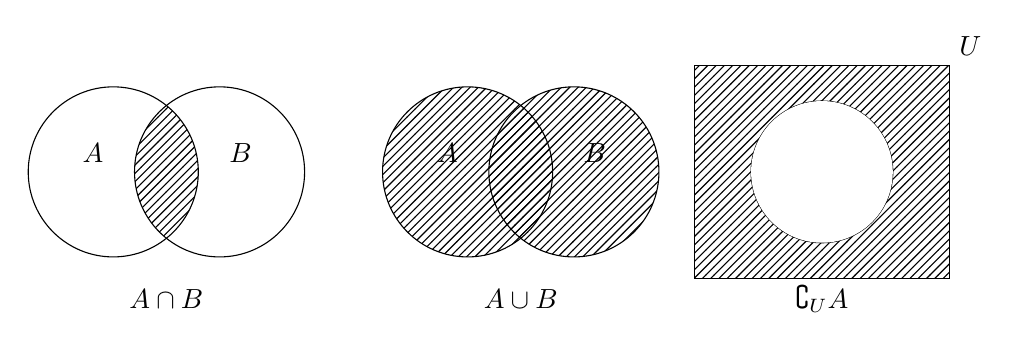
\begin{tikzpicture}[scale=0.9]
			% 交集
			\begin{scope}
				\draw (0,0) circle (1.2) node[above left] {$A$};
				\draw (1.5,0) circle (1.2) node[above right] {$B$};
				\begin{scope}
					\clip (0,0) circle (1.2);
					\fill[pattern=north east lines] (1.5,0) circle (1.2);
				\end{scope}
				\node at (0.75,-1.8) {$A \cap B$};
			\end{scope}
			
			% 并集
			\begin{scope}[xshift=5cm]
				\draw (0,0) circle (1.2) node[above left] {$A$};
				\draw (1.5,0) circle (1.2) node[above right] {$B$};
				\fill[pattern=north east lines] (0,0) circle (1.2);
				\fill[pattern=north east lines] (1.5,0) circle (1.2);
				\node at (0.75,-1.8) {$A \cup B$};
			\end{scope}
			
			% 补集
			\begin{scope}[xshift=10cm]
				\draw (-1.8,-1.5) rectangle (1.8,1.5) node[above right] {$U$};
				\draw (0,0) circle (1) node {$A$};
				\begin{scope}
					\clip (-1.8,-1.5) rectangle (1.8,1.5);
					\fill[pattern=north east lines] (-1.8,-1.5) rectangle (1.8,1.5);
					\fill[white] (0,0) circle (1);
				\end{scope}
				\node at (0,-1.8) {$\complement_U A$};
			\end{scope}
		\end{tikzpicture}
		\caption{交集、并集与补集的韦恩图表示}
	\end{figure}
	
	\begin{property}[集合运算律]
		\begin{enumerate}
			\item 交换律:$A \cap B = B \cap A$; $A \cup B = B \cup A$
			\item 结合律:$(A \cap B) \cap C = A \cap (B \cap C)$; $(A \cup B) \cup C = A \cup (B \cup C)$
			\item 分配律:$A \cap (B \cup C) = (A \cap B) \cup (A \cap C)$; $A \cup (B \cap C) = (A \cup B) \cap (A \cup C)$
		\end{enumerate}
	\end{property}
	
	\begin{note}[重要结论转换]
		集合的运算与包含关系可以相互转化,这在解决抽象集合问题时尤为关键:
		\begin{itemize}
			\item $A \cap B = A \iff A \subseteq B$
			\item $A \cup B = B \iff A \subseteq B$
			\item $A \cap (\complement_U B) = \emptyset \iff A \subseteq B$
		\end{itemize}
	\end{note}
	
	\section{常用逻辑用语}
	
	逻辑是数学严谨性的保证,本节将帮助你理清命题关系,准确判断条件.
	
	\subsection{命题及其关系}
	
	\begin{definition}[命题]
		能够判断真假的陈述句称为\textbf{命题}.真命题的真值为真,假命题的真值为假.
	\end{definition}
	
	对于形如“若 $p$,则 $q$”的命题,$p$ 称为条件,$q$ 称为结论.
	
	\begin{definition}[四种命题] 
		以“若 $p$,则 $q$”为\textbf{原命题}:
		\begin{itemize}
			\item \textbf{逆命题}:若 $q$,则 $p$.(交换条件与结论)
			\item \textbf{否命题}:若非 $p$,则非 $q$.(否定条件与结论)
			\item \textbf{逆否命题}:若非 $q$,则非 $p$.(先交换,再否定)
		\end{itemize}
	\end{definition}
	
	\begin{theorem}[命题等价关系] 
		一个命题与它的逆否命题具有相同的真假性,它们是\textbf{等价}的.
		一个命题的逆命题与它的否命题也是等价的.
	\end{theorem}
	
	\begin{note}
		在高考中,对含有量词的命题进行否定是一个高频考点.无论原命题真假,其否定形式都遵循唯一法则:\textbf{换量词,否结论}.
		\begin{itemize}
			\item 否定全称命题“对\textbf{所有} $x$,$p(x)$ 都成立”:结果是特称命题“\textbf{存在}一个 $x_0$,使得 $p(x_0)$ \textbf{不}成立”.
			($\forall$ 变 $\exists$, $p(x)$ 变 $\neg p(x)$)
			\item 否定特称命题“\textbf{存在}一个 $x_0$,使得 $p(x_0)$ 成立”:结果是全称命题“对\textbf{所有} $x$,$p(x)$ 都\textbf{不}成立”.
			($\exists$ 变 $\forall$, $p(x)$ 变 $\neg p(x)$)
		\end{itemize}
	\end{note}
	
	\subsection{充分条件与必要条件}
	
	\begin{definition}[充分与必要条件]
		对于命题“若 $p$,则 $q$”:
		\begin{itemize}
			\item 如果该命题为真 ($p \Rightarrow q$),则称 $p$ 是 $q$ 的\textbf{充分条件},$q$ 是 $p$ 的\textbf{必要条件}.
			\item 如果 $p \Rightarrow q$ 但 $q \nRightarrow p$,则 $p$ 是 $q$ 的\textbf{充分不必要条件}.
			\item 如果 $p \nRightarrow q$ 但 $q \Rightarrow p$,则 $p$ 是 $q$ 的\textbf{必要不充分条件}.
			\item 如果 $p \iff q$,则 $p$ 是 $q$ 的\textbf{充分必要条件}(简称\textbf{充要条件}).
			\item 如果 $p \nRightarrow q$ 且 $q \nRightarrow p$,则 $p$ 是 $q$ 的\textbf{既不充分也不必要条件}.
		\end{itemize}
	\end{definition}
	
	\begin{note}[集合法]
		判断条件的类型,最直观有效的方法之一是“集合法”.将条件 $p$ 和结论 $q$ 看作两个集合 $A$ 和 $B$($A = \{x \mid p(x) \text{为真}\}$,$B = \{x \mid q(x) \text{为真}\}$),则:
		\begin{itemize}
			\item 若 $A \subsetneq B$,则 $p$ 是 $q$ 的充分不必要条件.
			\item 若 $B \subsetneq A$,则 $p$ 是 $q$ 的必要不充分条件.
			\item 若 $A = B$,则 $p$ 是 $q$ 的充要条件.
			\item 若 $A \not\subseteq B$ 且 $B \not\subseteq A$,则 $p$ 是 $q$ 的既不充分也不必要条件.
		\end{itemize}
		简记为:“小集推大集”,小范围是充分,大范围是必要.
	\end{note}
	
	\begin{conclusion}
		本章的集合与逻辑是数学世界的基础设施.集合提供了分类和组织信息的语言,逻辑则提供了推理和证明的规则.熟练地运用韦恩图、数轴分析集合关系,并将条件判断问题转化为集合包含问题,是高效解决本章考题的核心策略.
	\end{conclusion}
	\makechapteropener
	{三} 
	{不等式}
	{给我五个系数,我将画出一头大象;给我六个,我能让它的鼻子摇晃。} 
	{奥古斯丁·路易·柯西 (Augustin-Louis Cauchy)}
	
	\chapter{不等式}
	
	\lettrine{本}{章我们}将从最基础也最重要的一条不等式——基本不等式(均值不等式)出发,探索其内涵、证明与应用.我们将见识到著名的“调几代平”不等式链,更重要的是,我们将系统学习在求解最值问题时,那些令人拍案叫绝的“配凑”技巧,并掌握证明不等式的三大基本法门.攻克本章,你将获得解决优化问题的利器.
	
	% --- 章节摘要 ---
\begin{introduction}[知识概括]
	\item \textbf{均值不等式:} 深刻理解“一正、二定、三相等”的七字箴言,这是使用均值不等式求最值的大前提.本章的核心计算技巧均围绕“构造定值”这一目标展开.
	\item \textbf{不等式链:} 掌握“平方平均数 $\ge$ 算术平均数 $\ge$ 几何平均数 $\ge$ 调和平均数”这一重要结论,并理解其推导过程,它是不等式体系的延伸和完善.
	\item \textbf{配凑技巧:} 这是本章的灵魂.必须熟练掌握“拆项与凑项”、“凑系数”、“乘1代换”、“平方”等高级技巧,将非标准形式转化为可以应用均值不等式的标准形式.
	\item \textbf{证明方法:} 掌握作差法、分析法和综合法.理解分析法“执果索因”的思考路径与综合法“由因导果”的书写格式,是严谨证明不等式题目的关键.
\end{introduction}
	
	\section{均值不等式}
	
	\subsection{基本不等式}
	
	我们从一个简单而深刻的几何事实出发:对于一个长和宽分别为 $a,b$ 的矩形,其面积为 $ab$;而一个边长为 $\frac{a+b}{2}$ 的正方形,其面积为 $(\frac{a+b}{2})^2$.当周长固定时,正方形的面积最大.这一朴素的认知背后,蕴含着数学中最重要的不等式之一.
	
	\begin{theorem}[基本不等式]
		对于任意两个正实数 $a, b$,我们有:
		\begin{equation}
			\frac{a+b}{2} \ge \sqrt{ab}
		\end{equation}
		当且仅当 $a=b$ 时,等号成立.
	\end{theorem}
	
	\begin{proof}[证明]
		由于 $a, b$ 均为正实数,$\sqrt{a}$ 和 $\sqrt{b}$ 均有意义.
		我们知道,任何实数的平方都非负,所以:
		\begin{equation}
			(\sqrt{a} - \sqrt{b})^2 \ge 0
		\end{equation}
		展开得 $a - 2\sqrt{ab} + b \ge 0$,移项得 $a+b \ge 2\sqrt{ab}$.
		两边同时除以 2,即得 $\frac{a+b}{2} \ge \sqrt{ab}$.
		等号成立的条件是 $(\sqrt{a} - \sqrt{b})^2 = 0$,即 $\sqrt{a} = \sqrt{b}$,考虑到 $a, b$ 均为正数,故 $a=b$.
	\end{proof}
	\qed
	
			\begin{note}[七字箴言:一正、二定、三相等]
				使用基本不等式求最值,必须严格满足三个条件,缺一不可:
				\begin{enumerate}
					\item \textbf{一正}:所涉及的各项变量必须是正数.
					\item \textbf{二定}:在求最小值时,各项的和必须为定值;在求最大值时,各项的积必须为定值.
					\item \textbf{三相等}:取得最值的那个点,必须能使得不等式中的各项相等.如果等号永远取不到,那么最值就不是通过基本不等式求出的.
				\end{enumerate}
			\end{note}
			
			\subsection{均值不等式链 (调几代平)}
			
			基本不等式实际上是算术平均数与几何平均数的大小关系.将这个关系扩展,我们得到一条非常优美的不等式链.
			
			\begin{definition}[四种平均数]
				对于两个正数 $a,b$:
				\begin{itemize}
					\item \textbf{调和平均数 (H)}: $H_2 = \frac{2}{\frac{1}{a}+\frac{1}{b}}$
					\item \textbf{几何平均数 (G)}: $G_2 = \sqrt{ab}$
					\item \textbf{算术平均数 (A)}: $A_2 = \frac{a+b}{2}$
					\item \textbf{平方平均数 (Q)}: $Q_2 = \sqrt{\frac{a^2+b^2}{2}}$
				\end{itemize}
			\end{definition}
			
			\begin{theorem}[均值不等式链]
				对于任意两个正实数 $a,b$,有:
				\begin{equation}
					\sqrt{\frac{a^2+b^2}{2}} \ge \frac{a+b}{2} \ge \sqrt{ab} \ge \frac{2}{\frac{1}{a}+\frac{1}{b}}
				\end{equation}
				即 $Q_2 \ge A_2 \ge G_2 \ge H_2$.当且仅当 $a=b$ 时,所有等号同时成立.
			\end{theorem}
			
			\begin{proof}
				我们已经证明了 $A_2 \ge G_2$.
				\begin{itemize}
					\item \textbf{证明 $Q_2 \ge A_2$}:
					作平方差:
					$Q_2^2 - A_2^2 = \frac{a^2+b^2}{2} - (\frac{a+b}{2})^2 = \frac{2(a^2+b^2) - (a^2+2ab+b^2)}{4} = \frac{a^2-2ab+b^2}{4} = \frac{(a-b)^2}{4} \ge 0$.
					因为 $Q_2, A_2$ 均为正,所以 $Q_2 \ge A_2$.当且仅当 $a=b$ 时取等.
					\item \textbf{证明 $G_2 \ge H_2$}:
					由于 $a,b$ 为正数,$\frac{1}{a}, \frac{1}{b}$ 也为正数.对其应用基本不等式:
					$\frac{\frac{1}{a}+\frac{1}{b}}{2} \ge \sqrt{\frac{1}{a} \cdot \frac{1}{b}} = \frac{1}{\sqrt{ab}}$.
					两边取倒数,并乘以 2,由于都是正数,不等号方向改变:
					$\frac{2}{\frac{1}{a}+\frac{1}{b}} \le \sqrt{ab}$.
					即 $H_2 \le G_2$.当且仅当 $\frac{1}{a}=\frac{1}{b}$,即 $a=b$ 时取等.
				\end{itemize}
				综上,不等式链成立.
			\end{proof}
			\qed

\section{不等式的配凑技巧与思想}

\subsection{方法论}

\textbf{【核心思想】}
\textcolor{green!50!black}{所有配凑技巧的出发点和归宿,都是为了同一个目标:\textbf{创造“定值”}.在使用均值不等式时,我们需要“和为定值”或“积为定值”;在使用柯西不等式时,我们需要某些“平方和”为定值.因此,解题的第一步,是敏锐地观察已知条件和所求表达式的结构特征.}
\begin{itemize}
	\item \textbf{看到分式,想到“拆”与“凑”}:尤其是分母是单项或简单多项式时,往往需要通过拆分分子或配凑系数,创造出与分母相乘为定值的项.
	\item \textbf{看到一次式条件,分式和所求}:形如已知 $ax+by=k$,求 $\frac{m}{x}+\frac{n}{y}$,这是“1的代换”的强烈信号.
	\item \textbf{看到二次式,想到配方与柯西}:条件或所求中出现 $x^2+y^2$ 等形式,优先考虑柯西不等式或二次函数配方法.
	\item \textbf{看到不同次的式子,想到齐次化}:当分式中分子分母次数不同,结构复杂时,考虑通过“除法”等手段,将其变为“整式+分式”的齐次结构.
\end{itemize}

\subsection{技巧一:拆项与凑项法(加减常数)}

\textbf{【原理与逻辑】}
这是最基本的配凑法.其原理在于,当我们有两个正变量 $u,v$,直接使用均值不等式要求 $u+v$ 或 $uv$ 是定值.当它们不是定值时,我们就需要主动去改造其中一个变量.例如,对于 $f(x)=g(x)+\frac{k}{h(x)}$,若 $g(x) \cdot \frac{k}{h(x)}$ 不是常数,我们就想办法把 $g(x)$ 变形为 $c \cdot h(x) + \text{常数}$ 的形式,这样 $c \cdot h(x) \cdot \frac{k}{h(x)}$ 就成了常数.

\begin{exercise}[基础]
	已知 $x>2$,求函数 $f(x) = x + \frac{1}{x-2}$ 的最小值.
\end{exercise}
\begin{solution}
	\textcolor{green!50!black}{直接对 $x$ 和 $\frac{1}{x-2}$ 使用均值不等式,其乘积为 $\frac{x}{x-2}$,不是定值.观察到分母是 $x-2$,我们希望分子中也出现一个 $(x-2)$ 项来与之相乘,从而消去变量.}
	将 $x$ 拆分为 $(x-2)+2$.
		$f(x) = (x-2) + \frac{1}{x-2} + 2$
		
		因为 $x>2$,所以 $x-2 > 0$.\textcolor{red}{(“一正”条件满足)}
		对前两项应用均值不等式:
		$(x-2) + \frac{1}{x-2} \ge 2\sqrt{(x-2) \cdot \frac{1}{x-2}} = 2\sqrt{1} = 2$.
		\textcolor{red}{(“二定”条件,积为定值1,已满足)}
		
		所以 $f(x) \ge 2+2=4$.

		当且仅当 $(x-2) = \frac{1}{x-2}$,即 $(x-2)^2=1$,解得 $x-2=1$(因为$x-2>0$),即 $x=3$ 时,等号成立.\textcolor{red}{(“三相等”条件满足)}
	函数的最小值为 $\textcolor{red}{4}$.
\end{solution}
\qed

\subsection{“对勾函数”模型}
形如 $f(x)=x+\frac{a}{x} \ (a>0)$ 的函数被称为“对勾函数”,因其图像形似一个对勾.
\begin{itemize}
	\item \textbf{定义域}: $(-\infty, 0) \cup (0, +\infty)$
	\item \textbf{奇偶性}: 奇函数,图像关于原点对称.
	\item \textbf{单调性}: 在 $(0, \sqrt{a}]$ 上单调递减,在 $[\sqrt{a}, +\infty)$ 上单调递增;在 $(-\infty, -\sqrt{a}]$ 上单调递增,在 $[-\sqrt{a}, 0)$ 上单调递减.
	\item \textbf{最值}: 当 $x>0$ 时,在 $x=\sqrt{a}$ 处取得最小值 $2\sqrt{a}$;当 $x<0$ 时,在 $x=-\sqrt{a}$ 处取得最大值 $-2\sqrt{a}$.
\end{itemize}
\begin{figure}[H]
	\centering
	\begin{tikzpicture}[scale=0.8]
		\draw[->] (-5,0) -- (5,0) node[below] {$x$};
		\draw[->] (0,-5) -- (0,5) node[left] {$y$};
		\draw[blue, thick, smooth] plot[domain=0.5:4] (\x, {\x+4/\x});
		\draw[blue, thick, smooth] plot[domain=-4:-0.5] (\x, {\x+4/\x});
		\node[blue, right] at (4,5) {$y=x+\frac{4}{x}$};
		\fill[red] (2,4) circle (2pt) node[right] {$(2,4)$};
		\fill[red] (-2,-4) circle (2pt) node[left] {$(-2,-4)$};
	\end{tikzpicture}
	\caption{对勾函数图像}
\end{figure}
\textcolor{green!50!black}{理解对勾函数模型,可以帮助我们快速判断形如 $g(x)+k/g(x)$ 的函数的单调性,以及在等号取不到时,确定最值是在端点取到还是不存在.}

\subsection{技巧二:“1”的代换法(乘“1”代换)}

\textcolor{green!50!black}{为什么“1的代换”如此有效?其本质是\textbf{次数的配平}.}
考虑一个典型问题:已知 $x+2y=1$(这是一个\textbf{1次式}),求 $\frac{1}{x}+\frac{1}{y}$(这是一个\textbf{-1次式})的最小值.
如果我们直接将两者相乘:$(\frac{1}{x}+\frac{1}{y})(x+2y)$,展开后得到的项 $1, \frac{2y}{x}, \frac{x}{y}, 2$ 都是\textbf{0次式}!
其中,$1$ 和 $2$ 是常数项(定值),而 $\frac{2y}{x}$ 和 $\frac{x}{y}$ 是互为倒数关系的项,它们的乘积也是定值.
\textcolor{green!50!black}{结论:将一个-1次的表达式乘以一个1次的条件式,可以“配平”次数,将问题转化为处理我们最喜欢的0次式(常数和倒数),这正是均值不等式的最佳用武之地.}

\begin{exercise}
	已知正数 $x,y$ 满足 $x+2y=1$,求 $\frac{1}{x} + \frac{1}{y}$ 的最小值.
\end{exercise}
\begin{solution}
	\textcolor{green!50!black}{这是一个典型的“和为定值,求分式和最值”问题.直接通分或使用均值不等式都会失败.这正是“1的代换”的标志性信号.}
	\begin{enumerate}
		\item \textbf{乘“1”代换}:
		$\frac{1}{x} + \frac{1}{y} = \left( \frac{1}{x} + \frac{1}{y} \right) \cdot 1 = \left( \frac{1}{x} + \frac{1}{y} \right) (x+2y)$
		
		\item \textbf{展开}:
		$= \frac{x}{x} + \frac{2y}{x} + \frac{x}{y} + \frac{2y}{y} = 1 + \frac{2y}{x} + \frac{x}{y} + 2 = 3 + \left( \frac{2y}{x} + \frac{x}{y} \right)$
		
		\item \textbf{使用均值不等式}:
		因为 $x,y$ 为正数, 所以 $\frac{2y}{x} > 0, \frac{x}{y} > 0$.
		对括号内部分使用均值不等式:
		$\frac{2y}{x} + \frac{x}{y} \ge 2\sqrt{\frac{2y}{x} \cdot \frac{x}{y}} = 2\sqrt{2}$
		
		\item \textbf{得出最小值}:
		所以 $\frac{1}{x} + \frac{1}{y} \ge 3 + 2\sqrt{2}$.
		
		\item \textbf{检验等号}:
		当且仅当 $\frac{2y}{x} = \frac{x}{y}$,即 $x^2 = 2y^2$, $x = \sqrt{2}y$ 时取等.
		代入 $x+2y=1$ 中,有 $\sqrt{2}y+2y=1$, 解得 $y = \frac{1}{2+\sqrt{2}}$.存在这样的 $x,y$.
	\end{enumerate}
	$\frac{1}{x} + \frac{1}{y}$ 的最小值为 $\textcolor{red}{3 + 2\sqrt{2}}$.
\end{solution}
\qed

\subsection{技巧三:齐次化(分离常数)}
当遇到形如 $\frac{ax^2+bx+c}{dx+e}$ 的分式,分子分母次数不同,结构不整齐,直接使用任何不等式都很困难.齐次化的思想,是通过\textbf{多项式除法}或类似方法,将其分离成“\textbf{整式 + 真分式}”的结构.这样处理后,往往能转化成我们熟悉的、可以使用拆凑法或均值不等式的形式.

\begin{exercise}
	已知 $x>0$,求 $f(x) = \frac{x^2+2x+5}{x+1}$ 的最小值.
\end{exercise}
\begin{solution}
	\textcolor{green!50!black}{分子是二次,分母是一次,次数不同.我们需要齐次化.方法一是用多项式长除法;方法二是在分子中“配凑”出分母的因式.}
	\begin{enumerate}
		\item \textbf{分子配凑}:
		$f(x) = \frac{x^2+2x+5}{x+1} = \frac{x(x+1)+x+5}{x+1} = x + \frac{x+5}{x+1}$
		\textcolor{green!50!black}{还不够,继续对剩下的分式进行配凑.}
		$f(x) = x + \frac{(x+1)+4}{x+1} = x + 1 + \frac{4}{x+1}$
		
		\item \textbf{转化为拆凑法问题}:
		现在问题变成了求 $(x+1)+\frac{4}{x+1}$ 的最小值.
		令 $t=x+1$,因为 $x>0$,所以 $t>1$.问题是求 $t+\frac{4}{t}$ 在 $t \in (1, \infty)$ 的最小值.
		
		\item \textbf{使用均值不等式}:
		因为 $t>0$, 所以 $t+\frac{4}{t} \ge 2\sqrt{t\cdot\frac{4}{t}} = 4$.
		
		\item \textbf{检验等号}:
		当且仅当 $t = \frac{4}{t}$,即 $t^2=4, t=2$ (因 $t>0$).
		$t=2$ 对应 $x+1=2 \implies x=1$.
		因为 $x=1$ 在定义域 $x>0$ 内,所以等号可取.
	\end{enumerate}
	最小值为 $\textcolor{red}{4}$.
\end{solution}
\qed

\subsection{技巧四:柯西不等式的配凑}

柯西不等式的配凑比均值不等式更灵活.当我们面对的目标函数或约束条件,可以通过“开方”或“平方”凑成柯西不等式的标准形式 $(a^2+b^2)(x^2+y^2) \ge (ax+by)^2$ 时,就可以考虑使用它.

\begin{exercise}
	已知 $x,y$ 均为正数,且 $x+2y=xy$,求 $2x+y$ 的最小值.
\end{exercise}
\begin{solution}
	\textcolor{green!50!black}{这个条件 $x+2y=xy$ 非常不寻常.直接处理很困难.我们可以尝试对它进行变形.两边同除以 $xy$ (因为 $x,y$ 为正数,可以除),看看能得到什么.}
	\begin{enumerate}
		\item \textbf{变形条件}:
		$x+2y=xy \implies \frac{x}{xy} + \frac{2y}{xy} = 1 \implies \frac{1}{y} + \frac{2}{x} = 1$.
		\textcolor{green!50!black}{现在条件变成了一个我们熟悉的“分式和为定值”的形式.}
		
		\item \textbf{构造柯西不等式}:
		我们要求 $2x+y$ 的最小值.
		我们有两个部分:条件 $\frac{2}{x}+\frac{1}{y}=1$ 和目标 $2x+y$.
		考虑使用“1的代换”,但是这次我们用柯西不等式来处理.
		设 $S = 2x+y$.
		$S = S \cdot 1 = (2x+y)(\frac{2}{x}+\frac{1}{y})$.展开后不是很好处理.
		
		\textbf{尝试直接构造柯西不等式:}
		$S = (\sqrt{2x})^2 + (\sqrt{y})^2$.
		条件是 $\frac{2}{x}+\frac{1}{y} = (\frac{\sqrt{2}}{\sqrt{x}})^2 + (\frac{1}{\sqrt{y}})^2 = 1$.
		
		套用柯西不等式 $(a^2+b^2)(x^2+y^2) \ge (ax+by)^2$:
		令 $a=\sqrt{2x}, b=\sqrt{y}$; $x'=\frac{\sqrt{2}}{\sqrt{x}}, y'=\frac{1}{\sqrt{y}}$.
		$(a^2+b^2)(x'^2+y'^2) \ge (ax'+by')^2$
		
		\item \textbf{代入并计算}:
		$(2x+y) \left( \frac{2}{x}+\frac{1}{y} \right) \ge \left( \sqrt{2x}\cdot\frac{\sqrt{2}}{\sqrt{x}} + \sqrt{y}\cdot\frac{1}{\sqrt{y}} \right)^2$
		$(2x+y) \cdot 1 \ge (2+1)^2 = 9$.
		
		\item \textbf{得出最小值}:
		所以 $2x+y \ge 9$.
		
		\item \textbf{检验等号}:
		当且仅当 $\frac{\sqrt{2x}}{\sqrt{2}/\sqrt{x}} = \frac{\sqrt{y}}{1/\sqrt{y}}$.
		$\frac{\sqrt{2x}\sqrt{x}}{\sqrt{2}} = \frac{\sqrt{y}\sqrt{y}}{1} \implies x=y$.
		代入条件 $\frac{2}{x}+\frac{1}{y}=1$ 中:
		$\frac{2}{x}+\frac{1}{x}=1 \implies \frac{3}{x}=1 \implies x=3$.
		所以 $x=y=3$ 时,等号成立.
	\end{enumerate}
	\textbf{【最终答案】} $2x+y$ 的最小值为 $\textcolor{red}{9}$.
\end{solution}
\qed

\section{观察次数大作战}

	欢迎来到“观察次数大作战”!在这里,我们将把“配凑”的艺术提升到一个新的层次.我们不再仅仅是机械地进行拆项、凑系数,而是要学会用一双“火眼金睛”去\textbf{观察代数式中各项的“次数”}.
	\textbf{核心战术思想}:均值不等式的威力,在于它能处理“和”与“积”的关系.而当我们发现,若将若干项相乘,它们的变量可以互相抵消,最终得到一个常数(我们称之为“\textbf{零次式}”)时,均值不等式的大门就向我们敞开了.
	例如,对于 $x$ 和 $\frac{1}{x}$,我们可以非正式地认为它们的次数分别是 \textbf{1次} 和 \textbf{-1次}.它们的乘积 $x \cdot \frac{1}{x} = 1$ 就是一个 \textbf{0次} 的常数.
	本节的挑战,就是训练你通过观察和调整各项的“次数”,使其乘积变为“0次式”,从而克敌制胜!准备好了吗?战斗开始!

% \degree{次数}{表达式}
\newcommand{\degree}[2]{%
	\tikz[baseline=(M.base)] {
		\node[inner sep=0pt] (M) {$#2$}; 
		\node[draw, circle, red, inner sep=1pt, font=\tiny, above=1.5pt] at (M.north) {$#1$}; 
	}%
}

\begin{problemset}
	
	\item \textbf{[第一关]} 已知 $x>0$,求函数 $f(x) = x^2 + \frac{2}{x}$ 的最小值.
	
	\item \textbf{[第二关]} 已知 $x>-2$,求函数 $f(x) = \frac{x^2+5}{x+2}$ 的最小值.
	
	\item \textbf{[第三关]} 已知正数 $x,y$ 满足 $x+3y=2$,求 $\frac{2}{x}+\frac{3}{y}$ 的最小值.
	
	\item \textbf{[第四关]} 已知 $x>0, y>0$ 且 $x+y=1$,求 $\frac{1}{x^2}+\frac{1}{y^2}$ 的最小值.
	
	\item \textbf{[最终关]} 已知正数 $x,y,z$ 满足 $2x+y+z=4$,求 $x^2+\frac{y^2}{2}+z^2$ 的最小值.
	
\end{problemset}

\newpage

\begin{note}[“观察次数大作战”参考答案]
\end{note}

\begin{solution}
	\textbf{第一关参考答案}
	
	\textcolor{green!50!black}{观察次数!函数由 \degree{2}{x^2} 和 \degree{-1}{\frac{2}{x}} 两部分构成.直接相乘,次数为 $2+(-1)=1$,不是定值.为了让乘积变为“0次式”,我们需要用一个“2次项”去配平两个“-1次项”.这启发我们将 $\frac{2}{x}$ 拆成两项.}
	
		我们将原式拆分为:
		$f(x) = \degree{2}{x^2} + \degree{-1}{\frac{1}{x}} + \degree{-1}{\frac{1}{x}}$
		现在,三项的乘积次数为 $2+(-1)+(-1)=0$,它们的乘积为 $x^2 \cdot \frac{1}{x} \cdot \frac{1}{x} = 1$,是定值!
		
		因为 $x>0$,所以三项均为正数.
		$x^2 + \frac{1}{x} + \frac{1}{x} \ge 3\sqrt[3]{x^2 \cdot \frac{1}{x} \cdot \frac{1}{x}} = 3\sqrt[3]{1} = 3$

		当且仅当各项相等时,即 $x^2 = \frac{1}{x}$,解得 $x^3=1$,即 $x=1$ 时,等号成立.
	函数的最小值为 $\textcolor{red}{3}$.
\end{solution}
\qed
\begin{solution}
	\textbf{第二关参考答案}
	
	\textcolor{green!50!black}{观察次数!这是一个“2次/1次”型的分式,结构不整齐.我们的目标是将其转化为“\textbf{整式+分式}”的形式,使得整式部分和分式部分的次数能够平衡.这需要用到“分离常数”或“配凑分母”的技巧.}
	
		我们希望在分子中凑出 $(x+2)$ 的因式.
		$f(x) = \frac{x^2+5}{x+2} = \frac{(x^2-4)+9}{x+2} = \frac{(x-2)(x+2)}{x+2} + \frac{9}{x+2} = x-2+\frac{9}{x+2}$

		变形后的表达式为 $(x-2)+\frac{9}{x+2}$,它们的次数分别是 \degree{1}{x-2} 和 \degree{-1}{\frac{9}{x+2}},但变量部分 $x-2$ 和 $x+2$ 不同,无法直接对消.我们需要让变量部分完全一样.
		$f(x) = (x+2) - 4 + \frac{9}{x+2} = \left( \degree{1}{(x+2)} + \degree{-1}{\frac{9}{x+2}} \right) - 4$
		现在,括号内两项的乘积次数为 $1+(-1)=0$,乘积为定值 $9$.
		
		因为 $x>-2$,所以 $x+2>0$.
		$(x+2) + \frac{9}{x+2} \ge 2\sqrt{(x+2) \cdot \frac{9}{x+2}} = 2\sqrt{9} = 6$
		
		所以 $f(x) \ge 6-4=2$.
		
		当且仅当 $x+2 = \frac{9}{x+2}$,即 $(x+2)^2=9$,解得 $x+2=3$ (因为$x+2>0$),即 $x=1$ 时,等号成立.
	函数的最小值为 $\textcolor{red}{2}$.
\end{solution}
\qed
\begin{solution}
	\textbf{第三关参考答案}
	
	\textcolor{green!50!black}{观察次数!条件 $x+3y=2$ 是一个 \degree{1}{} 式,所求 $\frac{2}{x}+\frac{3}{y}$ 是一个 \degree{-1}{} 式.当一个“1次”的条件和一个“-1次”的目标同时出现时,这是一个强烈的信号:使用“\textbf{1的代换}”!将两者相乘,得到的将是一个“0次式”的乐园.}
	
		因为 $x+3y=2$,所以 $\frac{x+3y}{2}=1$.
		$\frac{2}{x}+\frac{3}{y} = \left(\frac{2}{x}+\frac{3}{y}\right) \cdot 1 = \left(\frac{2}{x}+\frac{3}{y}\right) \cdot \frac{x+3y}{2}$
		
		$= \frac{1}{2} \left( \frac{2x}{x} + \frac{6y}{x} + \frac{3x}{y} + \frac{9y}{y} \right)$
		$= \frac{1}{2} \left( \degree{0}{2} + \degree{0}{\frac{6y}{x}} + \degree{0}{\frac{3x}{y}} + \degree{0}{9} \right)$
		\textcolor{green!50!black}{看!展开后所有项都是“0次式”,其中 $\frac{6y}{x}$ 和 $\frac{3x}{y}$ 互为倒数关系,乘积为定值!}

		$= \frac{1}{2} \left( 11 + \frac{6y}{x} + \frac{3x}{y} \right)$
		$\ge \frac{1}{2} \left( 11 + 2\sqrt{\frac{6y}{x} \cdot \frac{3x}{y}} \right) = \frac{1}{2}(11+2\sqrt{18}) = \frac{11+6\sqrt{2}}{2}$
		
		当且仅当 $\frac{6y}{x}=\frac{3x}{y}$,即 $6y^2=3x^2 \implies x^2=2y^2 \implies x=\sqrt{2}y$ (因$x,y>0$)时取等.
		代入 $x+3y=2$ 得 $\sqrt{2}y+3y=2$,可解出正数 $y$,故等号可取.
	最小值为 $\textcolor{red}{\frac{11+6\sqrt{2}}{2}}$.
\end{solution}
\qed
\begin{solution}
	\textbf{第四关参考答案}

	\textcolor{green!50!black}{观察次数!目标是 \degree{-2}{\frac{1}{x^2}} 和 \degree{-2}{\frac{1}{y^2}} 的和,条件是 \degree{1}{x+y=1}.次数差异巨大,直接配凑极为困难.这提示我们不能只局限于简单的均值不等式,而要动用更根本的武器:\textbf{变量代换与函数思想},将双变量问题转化为单变量的函数最值问题,实现“降维打击”!}

		首先通分,将目标表达式化为一个整体:
		$\frac{1}{x^2} + \frac{1}{y^2} = \frac{x^2+y^2}{x^2y^2} = \frac{x^2+y^2}{(xy)^2}$
		
		我们用条件 $x+y=1$ 来表示分子和分母.
		分子:$x^2+y^2 = (x+y)^2 - 2xy = 1^2 - 2xy = 1-2xy$.
		所以,原式 $= \frac{1-2xy}{(xy)^2}$.

		\textcolor{blue}{整个表达式只与 $xy$ 有关,这是一个强烈的换元信号!}
		令 $t=xy$. 
		所求表达式变为 $f(t) = \frac{1-2t}{t^2}$.

		因为 $x>0, y>0$ 且 $x+y=1$,由均值不等式得:
		$1 = x+y \ge 2\sqrt{xy}$,所以 $1 \ge 4xy \implies xy \le \frac{1}{4}$.
		等号当且仅当 $x=y=\frac{1}{2}$ 时成立.
		所以新变量 $t$ 的取值范围是 $\textcolor{blue}{t \in (0, \frac{1}{4}]}$.

		$f(t) = \frac{1}{t^2} - \frac{2t}{t^2} = \frac{1}{t^2} - \frac{2}{t}$.
		这是一个关于 $\frac{1}{t}$ 的二次函数.令 $u = \frac{1}{t}$,由于 $t \in (0, \frac{1}{4}]$,所以 $\textcolor{blue}{u \in [4, +\infty)}$.
		问题转化为求函数 $g(u) = u^2 - 2u$ 在 $u \in [4, +\infty)$ 上的最小值.
	
		配方得 $g(u) = (u-1)^2 - 1$. 这是一个开口向上,对称轴为 $u=1$ 的抛物线.
		在区间 $[4, +\infty)$上,函数 $g(u)$ 是\textbf{单调递增}的.
		因此,最小值在区间的左端点 $u=4$ 处取得.
		$g(u)_{\min} = g(4) = 4^2 - 2(4) = 16-8=8$.

	$\frac{1}{x^2}+\frac{1}{y^2}$ 的最小值为 $\textcolor{red}{8}$.
\end{solution}
\qed
\begin{solution}
	\textbf{最终关参考答案}
	
	\textcolor{green!50!black}{观察次数!条件 $2x+y+z=4$ 是一个 \degree{1}{} 式,目标 $x^2+\frac{y^2}{2}+z^2$ 是一个 \degree{2}{} 式的和.当“1次式”和“2次平方和”这两种结构同时出现时,这便是\textbf{柯西不等式}登场的最佳时机!我们的任务是巧妙构造,使其完美匹配柯西不等式的形式.}

		柯西不等式三维形式为:$(a^2+b^2+c^2)(u^2+v^2+w^2) \ge (au+bv+cw)^2$.
		我们的目标是 $x^2+\frac{y^2}{2}+z^2 = (\degree{1}{x})^2 + (\frac{\degree{1}{y}}{\sqrt{2}})^2 + (\degree{1}{z})^2$.
		这可以看作是 $u^2+v^2+w^2$ 部分,其中 $u=x, v=\frac{y}{\sqrt{2}}, w=z$.
		
		我们的条件是 $2x+y+z=4$,这要成为 $au+bv+cw$ 部分.
		$au+bv+cw = a(x) + b(\frac{y}{\sqrt{2}}) + c(z) = 2x+y+z$

		通过对比系数,我们可以解出 $a,b,c$:
		$ax = 2x \implies a=2$
		$\frac{by}{\sqrt{2}} = y \implies b=\sqrt{2}$
		$cz=z \implies c=1$

		现在,我们将 $a=2, b=\sqrt{2}, c=1$ 和 $u=x, v=\frac{y}{\sqrt{2}}, w=z$ 代入柯西不等式:
		$\left[ 2^2 + (\sqrt{2})^2 + 1^2 \right] \left[ x^2 + (\frac{y}{\sqrt{2}})^2 + z^2 \right] \ge \left( 2x + \sqrt{2}\cdot\frac{y}{\sqrt{2}} + 1\cdot z \right)^2$

		$(4+2+1) \left( x^2+\frac{y^2}{2}+z^2 \right) \ge (2x+y+z)^2$
		$7 \left( x^2+\frac{y^2}{2}+z^2 \right) \ge 4^2 = 16$
		$x^2+\frac{y^2}{2}+z^2 \ge \frac{16}{7}$

		当且仅当 $\frac{u}{a}=\frac{v}{b}=\frac{w}{c}$,即 $\frac{x}{2} = \frac{y/\sqrt{2}}{\sqrt{2}} = \frac{z}{1}$.
		$\frac{x}{2} = \frac{y}{2} = \frac{z}{1}$.
		令其比值为 $k$,则 $x=2k, y=2k, z=k$.
		代入 $2x+y+z=4$ 得 $2(2k)+2k+k=4 \implies 7k=4 \implies k=\frac{4}{7}$.
		可以解出正数 $x,y,z$,故等号可取.

	最小值为 $\textcolor{red}{\frac{16}{7}}$.
\end{solution}
\qed

\section{不等式证明的基本方法}

\begin{definition}[作差法]
	要证明 $A \ge B$,只需证明 $A-B \ge 0$.这是证明不等式最基本、最直接的方法.其步骤是:\textbf{作差 $\rightarrow$ 变形(因式分解、配方)$\rightarrow$ 判断符号}.
\end{definition}

\begin{definition}[分析法与综合法]
	\begin{itemize}
		\item \textbf{分析法}:从\textbf{求证}的不等式出发,寻求使其成立的\textbf{充分条件},一步步回溯,直到找到一个已知条件、定义、公理或已被证明的定理为止.其书写格式为:“欲证...,只需证...,即证...”.分析法是\textbf{思考发现}路径的方法.
		\item \textbf{综合法}:从\textbf{已知}条件或公理出发,通过一系列逻辑推导,最终得到\textbf{求证}的不等式.这是\textbf{书写证明}过程的标准方法.
	\end{itemize}
\end{definition}

\begin{note}[方法论]
	在解决复杂的证明题时,我们通常采用“两头凑”的策略:先用\textbf{分析法}找到从结论到条件的路径,理清思路;再用\textbf{综合法}按照发现的路径,从条件出发,条理清晰地写出证明过程.
\end{note}


\begin{conclusion}
	不等式是贯穿高中数学的一条重要主线.本章学习的核心,是以内功(基本不等式及证明三大法门)为基础,以外功(配凑技巧)为招式,内外兼修.面对最值问题,要时刻保持对“一正、二定、三相等”的警觉,主动去创造条件,而不是等待条件.掌握了不等式的思想,许多看似复杂的问题都会迎刃而解.
\end{conclusion}

\section{不等式的解法}

掌握不等式的性质和证明是“内功”,而熟练求解不同类型的不等式则是“招式”.不等式的解法是代数变形能力的基本功,是解决函数定义域、值域以及各类优化问题的基础.

\subsection{一元二次不等式}

一元二次不等式的解法,是所有复杂不等式求解的基础,其核心思想是利用二次函数图像的直观性.

\begin{definition}[十字相乘法]
	十字相乘法是分解二次三项式 $ax^2+bx+c$ 的常用技巧.
	\begin{enumerate}
		\item \textbf{首项与常数项分解}: 将二次项系数 $a$ 分解为 $a_1 a_2$,常数项 $c$ 分解为 $c_1 c_2$.
		\item \textbf{交叉相乘,和凑中项}: 验证交叉相乘之和 $a_1 c_2 + a_2 c_1$ 是否等于一次项系数 $b$.
		\item \textbf{写出因式}: 若相等,则原式可分解为 $(a_1x + c_1)(a_2x + c_2)$.
	\end{enumerate}
	例如,分解 $3x^2-10x+8$:
	\begin{center}
		\begin{tikzpicture}
			\node at (0,0.5) {$3x$};
			\node at (0,-0.5) {$x$};
			\node at (2,0.5) {$-4$};
			\node at (2,-0.5) {$-2$};
			\draw (0.3,0.5) -- (1.7,-0.5);
			\draw (0.3,-0.5) -- (1.7,0.5);
			\node[right, green!50!black] at (2.2, 0) {交叉乘积和: $(3x)(-2) + (x)(-4) = -6x-4x = -10x$};
		\end{tikzpicture}
	\end{center}
	因为和等于一次项,所以 $3x^2-10x+8 = (3x-4)(x-2)$.
\end{definition}

\begin{note}[解一元二次不等式的三步法]
	\begin{enumerate}
		\item \textbf{标准化}:化为 $ax^2+bx+c > 0$ (或 $<0$) 且 $a>0$ 的形式.
		\item \textbf{求根}:使用十字相乘法或求根公式分解因式,求出方程 $ax^2+bx+c=0$ 的根 $x_1, x_2$.
		\item \textbf{看图写解集}:根据二次函数图像,结合口诀“大于取两边,小于取中间”写出解集.
	\end{enumerate}
\end{note}

\subsection{高次与分式不等式}

对于高次和分式不等式,我们采用通用的\textbf{数轴标根法}(穿针引线法).

\begin{definition}[数轴标根法]
	\begin{enumerate}
		\item \textbf{标准化}:不等式一端化为0,另一端各因式最高次项系数化为正.
		\item \textbf{求根}:求出所有根,并在数轴上从小到大标出.
		\item \textbf{穿线}:从右上角开始,自右向左用曲线穿根.
		\item \textbf{定则}:遵循“\textbf{奇穿偶不穿}”原则.即遇到奇数重根则穿过数轴,遇到偶数重根则不穿过(在根处与数轴相切).
		\item \textbf{写解集}:根据不等号要求,取数轴上方 ($>0$) 或下方 ($<0$) 对应的区间.注意开闭区间.
	\end{enumerate}
\end{definition}

\begin{note}[分式不等式的转化]
	$\frac{f(x)}{g(x)} \ge 0 \iff f(x)g(x) \ge 0 \text{ 且 } g(x) \neq 0$.其余同理,核心是\textbf{保证分母不为零}.
\end{note}

\begin{exercise}[2025新高考II卷]
	若$x=2$是函数$f(x)=(x-1)(x-2)(x-a)$的极值点,则$f(0)=$?
\end{exercise}

\begin{solution}
	一个点是多项式函数的极值点,意味着该点处的一阶导数为零,即 $f'(2)=0$.
	此外,一个点是函数的根,又是函数的极值点,意味着函数图像在此点与x轴相切,这表明该点是一个\textbf{偶数次重根}.
	
	\textbf{法一:导数法}
	求函数 $f(x)$ 的导数:
	$f'(x) = [(x-1)(x-2)]'(x-a) + (x-1)(x-2)(x-a)'$
	$f'(x) = (2x-3)(x-a) + (x-1)(x-2)$
	因为 $x=2$ 是极值点,所以 $f'(2)=0$:
	$f'(2) = (2(2)-3)(2-a) + (2-1)(2-2) = (1)(2-a) + (1)(0) = 0$
	解得 $a=2$.
	
	\textbf{法二:函数图像分析法}
	函数 $f(x)$ 在 $x=2$ 处有一个根.若该点还是极值点,则函数图像必然在 $x=2$ 处与x轴相切,这意味着 $x=2$ 至少是一个二重根.
	要使 $(x-2)$ 成为二重根,必须有 $a=2$.
	
	两种方法均得到 $a=2$.此时函数为 $f(x)=(x-1)(x-2)^2$.
	我们可以用数轴标根法画出此函数的简图,来验证 $x=2$ 确为极值点.
	该函数的根为 $x=1$ (奇次根) 和 $x=2$ (偶次根).
	\begin{figure}[H]
		\centering
		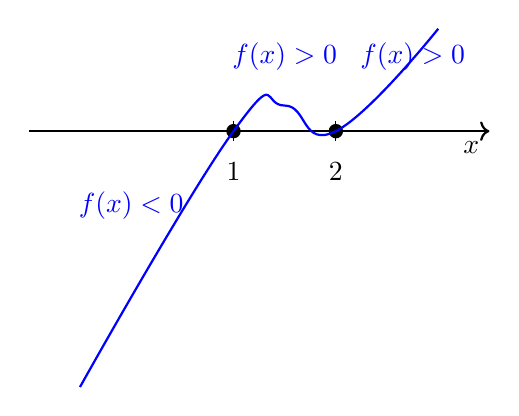
\begin{tikzpicture}[scale=1.3]
			\draw[->, thick] (-1,0) -- (3.5,0) node[below left] {$x$};
			
			\foreach \x/\label in {1/1, 2/2}{
				\draw (\x, 0.1) -- (\x, -0.1) node[below=4pt] {$\label$};
				\fill (\x,0) circle (2pt);
			}
			
			\draw[blue, thick] plot[smooth, tension=0.8] coordinates { (3, 1) (2,0) (1.5, 0.25) (1,0) (-0.5, -2.5) };
			
			\node[above, blue] at (2.75, 0.5) {$f(x)>0$};
			\node[above, blue] at (1.5, 0.5) {$f(x)>0$};
			\node[below, blue] at (0, -0.5) {$f(x)<0$};
			
		\end{tikzpicture}
		\caption{函数 $f(x)=(x-1)(x-2)^2$ 的图像示意}
	\end{figure}
	从上图可以清晰地看到,函数在 $x=2$ 点处触及x轴后并未穿过,形成了一个极小值点,符合题意.
	计算 $f(0)$:
	\begin{equation}
		f(0) = (0-1)(0-2)^2 = (-1)(4) = -4
	\end{equation}
	所以,最终答案是 -4.
\end{solution}
\qed


\subsection{含绝对值的不等式}

解含绝对值不等式的核心思想是“去掉绝对值符号”,主要有三种方法:

\begin{enumerate}
	\item \textbf{公式法}:利用基本模型 $|f(x)| < a \iff -a < f(x) < a$ 和 $|f(x)| > a \iff f(x) > a \text{ 或 } f(x) < -a$ (其中 $a>0$).
	\item \textbf{零点分段讨论法}:找到所有绝对值内部表达式的零点,用零点将数轴划分为若干区间,在每个区间上分别求解.
	\item \textbf{几何意义法}:利用 $|x-a|$ 表示数轴上点 $x$ 到点 $a$ 的距离.
\end{enumerate}

\begin{exercise}
	解不等式 $|x+1| - |x-2| \ge 1$.
\end{exercise}

\begin{solution}[零点分段法]
	零点为 $x=-1$ 和 $x=2$.它们将数轴分为三个区间,如图~\ref{fig:fenduan} 所示.
	
	\begin{itemize}
		\item \textbf{区间1 ($x < -1$)}:$-(x+1) + (x-2) \ge 1 \implies -3 \ge 1$.无解.
		\item \textbf{区间2 ($-1 \le x < 2$)}:$(x+1) + (x-2) \ge 1 \implies 2x-1 \ge 1 \implies x \ge 1$.取交集得 $1 \le x < 2$.
		\item \textbf{区间3 ($x \ge 2$)}:$(x+1) - (x-2) \ge 1 \implies 3 \ge 1$.恒成立.取交集得 $x \ge 2$.
	\end{itemize}
	综合所有区间的解,得到原不等式的解集为 $[1, \infty)$.
\end{solution}
\qed

\begin{figure}[H]
	\centering
	\begin{tikzpicture}[scale=1.2]
		% 坐标轴
		\draw[->, thick] (-3.5,0) -- (4.5,0) node[below left] {$x$};
		
		% 标出零点和分割线
		\foreach \x/\label in {-1/-1, 2/2}{
			\draw (\x, 0.2) -- (\x, -0.2) node[below=4pt] {$\label$};
			\draw[dashed] (\x, -0.5) -- (\x, 1.2);
		}
		
		% 标出区间名称
		\node[above] at (-2.25, 0.8) {区间1};
		\node[above] at (0.5, 0.8) {区间2};
		\node[above] at (3.25, 0.8) {区间3};
		
		% 标出最终解集
		\draw[line width=3pt, red] (1, -0.3) -- (4.5, -0.3);
		\fill[red] (1, -0.3) circle (2pt);
		\draw (1, -0.3) node[below=4pt, black] {$1$};
		\node[above, red] at (2.75, -0.3) {最终解集};
	\end{tikzpicture}
	\caption{零点分段法示意图}
\end{figure}

\section{柯西不等式}

如果说均值不等式是处理“和与积”问题的专家,那么柯西不等式则是一位处理“\textbf{平方和}”与“\textbf{和的平方}”之间关系的全能大师.它不受“正数”的限制(实数即可),形式灵活多变,威力巨大,在求最值、证不等式等领域都有着极其广泛的应用,被誉为“万能不等式”之一.掌握柯西不等式,将为你解决许多看似棘手的问题提供一个全新的、强有力的视角.


\subsection{柯西不等式的基本形式}

\begin{theorem}[柯西不等式二维形式]
	设 $a, b, x, y$ 均为实数,则:
	\begin{equation}
		\textcolor{red}{(a^2+b^2)(x^2+y^2) \ge (ax+by)^2}
	\end{equation}
	当且仅当 $\frac{a}{x} = \frac{b}{y}$ 时(或 $ay=bx$),等号成立.
\end{theorem}

\begin{theorem}[柯西不等式三维形式]
	设 $a, b, c, x, y, z$ 均为实数,则:
	\begin{equation}
		(a^2+b^2+c^2)(x^2+y^2+z^2) \ge (ax+by+cz)^2
	\end{equation}
	当且仅当 $\frac{a}{x} = \frac{b}{y} = \frac{c}{z}$ 时,等号成立.
\end{theorem}

\begin{note}
	该不等式可以推广到任意n维形式.在高中阶段,我们主要掌握其二维和三维形式的应用.其核心结构是:\textbf{(一堆数的平方和)乘以(另一堆数的平方和)大于等于(对应数乘积之和)的平方.}
\end{note}

\subsection{向量法证明}

\textcolor{green!50!black}{柯西不等式的结构与向量的坐标运算形式高度相似,这启发我们使用向量工具来证明它.向量法不仅形式上最为优美,也最能揭示不等式成立的几何本质.}

\begin{proof}[二维形式的向量证明]
		在平面直角坐标系中,我们构造两个向量:
		$\vec{m} = (a, b)$
		$\vec{n} = (x, y)$
		\begin{itemize}
			\item 代数表示:$\vec{m} \cdot \vec{n} = ax+by$
			\item 几何表示:$\vec{m} \cdot \vec{n} = |\vec{m}||\vec{n}|\cos\theta$,其中 $\theta$ 是两向量的夹角.
			\begin{figure}[H]
				\centering
				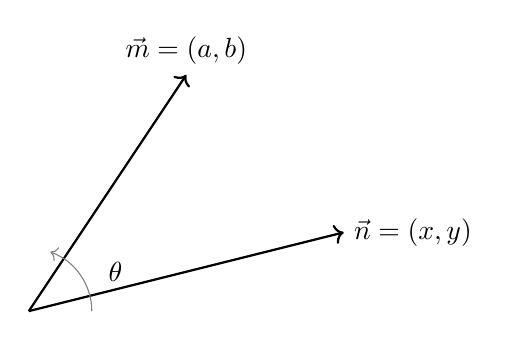
\begin{tikzpicture}
					\draw[->, thick] (0,0) -- (4,1) node[right] {$\vec{n}=(x,y)$};
					\draw[->, thick] (0,0) -- (2,3) node[above] {$\vec{m}=(a,b)$};
					\draw[->, gray] (0.8,0) arc (0:70:0.8);
					\node at (1.1, 0.5) {$\theta$};
				\end{tikzpicture}
				\caption{向量夹角示意图}
			\end{figure}
		\end{itemize}
		
		由数量积的两种表示相等,我们有:
		$ax+by = |\vec{m}||\vec{n}|\cos\theta$
		将两边同时平方,得到:
		$(ax+by)^2 = (|\vec{m}||\vec{n}|\cos\theta)^2 = |\vec{m}|^2 |\vec{n}|^2 \cos^2\theta$

		因为 $\cos^2\theta \le 1$,所以:
		$|\vec{m}|^2 |\vec{n}|^2 \cos^2\theta \le |\vec{m}|^2 |\vec{n}|^2$
		即 $(ax+by)^2 \le |\vec{m}|^2 |\vec{n}|^2$

		我们知道 $|\vec{m}|^2 = a^2+b^2$,$|\vec{n}|^2 = x^2+y^2$.
		代入上式,即得:
		$(ax+by)^2 \le (a^2+b^2)(x^2+y^2)$
		
		等号成立的条件是 $\cos^2\theta = 1$,这意味着 $\cos\theta = \pm 1$,即 $\theta=0$ 或 $\theta=\pi$.
		从几何上看,这意味着向量 $\vec{m}$ 与 $\vec{n}$ \textbf{共线}.
		从代数上看,共线意味着存在实数 $k$,使得 $\vec{m} = k\vec{n}$,即 $(a,b)=k(x,y)$.
		所以 $a=kx, b=ky$.当 $x,y$ 不为零时,即 $\frac{a}{x}=\frac{b}{y}=k$.
	三维形式的证明完全同理,只需构造三维向量 $\vec{m}=(a,b,c)$ 和 $\vec{n}=(x,y,z)$ 即可.
\end{proof}
\qed

\subsection{柯西不等式的信号与常见用法}

\textbf{【核心技巧】}
\textcolor{green!50!black}{如何判断一道题可能需要用到柯西不等式?关键是识别出题目中存在的“\textbf{平方和}”与“\textbf{一次式}”的结构.}
\begin{itemize}
	\item \textbf{信号一:题目条件或结论中出现 $x^2+y^2$ 或 $a^2+b^2+c^2$ 这样的平方和形式.}
	\item \textbf{信号二:题目条件或结论中出现 $ax+by$ 或 $ax+by+cz$ 这样的一次齐次式.}
\end{itemize}
柯西不等式的本质作用,就是建立起了这两种结构之间的桥梁:$(a^2+b^2)(x^2+y^2) \ge (ax+by)^2$.

\subsubsection{用法一:求最值}
这是柯西不等式在高考中最常见的应用.

\begin{exercise}
	已知实数 $x,y$ 满足 $3x+4y=10$,求 $x^2+y^2$ 的最小值.
\end{exercise}
\begin{solution}
	\textbf{【思路分析】}
	\textcolor{green!50!black}{我们观察到,条件是“一次式” ($3x+4y$),结论是求“平方和” ($x^2+y^2$) 的最值.这完美匹配了柯西不等式的结构.}
	
	\textbf{【解题步骤】}
	\begin{enumerate}
		\item \textbf{识别并构造不等式}:
		将 $3x+4y$ 看作 $ax+by$ 的形式,其中 $a=3, b=4$.
		将 $x^2+y^2$ 看作 $x^2+y^2$ 的形式.
		直接套用柯西不等式二维形式:
		$(a^2+b^2)(x^2+y^2) \ge (ax+by)^2$
		
		\item \textbf{代入已知量}:
		$(3^2+4^2)(x^2+y^2) \ge (3x+4y)^2$
		$25(x^2+y^2) \ge (10)^2$
		$25(x^2+y^2) \ge 100$
		
		\item \textbf{求解最值}:
		$x^2+y^2 \ge 4$
		所以 $x^2+y^2$ 的最小值为4.
		
		\item \textbf{【易错陷阱】检验等号能否取到}:
		\textcolor{red}{任何用不等式求出的最值,都必须验证其等号成立的条件能否满足,否则只是一个界,不一定是最值.}
		柯西不等式取等的条件是 $\frac{x}{a} = \frac{y}{b}$,在本题中即 $\frac{x}{3} = \frac{y}{4}$.
		设 $\frac{x}{3} = \frac{y}{4} = k$,则 $x=3k, y=4k$.
		将此代入约束条件 $3x+4y=10$ 中:
		$3(3k) + 4(4k) = 10 \implies 9k+16k=10 \implies 25k=10 \implies k=\frac{2}{5}$.
		此时,$x=3k=\frac{6}{5}, y=4k=\frac{8}{5}$.
		因为能找到具体的 $x,y$ 使等号成立,所以最小值确实是4.
	\end{enumerate}
	\textbf{【最终答案】} $x^2+y^2$ 的最小值为 $\textcolor{red}{4}$.
\end{solution}
\qed

\subsubsection{用法二:证明不等式}
柯西不等式是证明某些特定结构不等式的利器.

\begin{exercise}
	已知 $a,b,c$ 均为正数,求证:$(a+b+c)(\frac{1}{a}+\frac{1}{b}+\frac{1}{c}) \ge 9$.
\end{exercise}
\begin{solution}
	\textbf{【思路分析】}
	\textcolor{green!50!black}{这个不等式虽然可以用均值不等式证明,但用柯西不等式会更加直接.关键在于如何看出柯西不等式的结构.我们可以通过“开方配凑”的方法.}
	
	\textbf{【解题步骤】}
	\begin{enumerate}
		\item \textbf{构造平方和}:
		将 $a+b+c$ 看作 $(\sqrt{a})^2 + (\sqrt{b})^2 + (\sqrt{c})^2$.
		将 $\frac{1}{a}+\frac{1}{b}+\frac{1}{c}$ 看作 $(\frac{1}{\sqrt{a}})^2 + (\frac{1}{\sqrt{b}})^2 + (\frac{1}{\sqrt{c}})^2$.
		
		\item \textbf{套用三维柯西不等式}:
		设 $x_1=\sqrt{a}, x_2=\sqrt{b}, x_3=\sqrt{c}$
		设 $y_1=\frac{1}{\sqrt{a}}, y_2=\frac{1}{\sqrt{b}}, y_3=\frac{1}{\sqrt{c}}$
		
		$(x_1^2+x_2^2+x_3^2)(y_1^2+y_2^2+y_3^2) \ge (x_1y_1+x_2y_2+x_3y_3)^2$
		
		\item \textbf{代入并计算}:
		左边即为 $(a+b+c)(\frac{1}{a}+\frac{1}{b}+\frac{1}{c})$.
		右边为 $(\sqrt{a}\cdot\frac{1}{\sqrt{a}} + \sqrt{b}\cdot\frac{1}{\sqrt{b}} + \sqrt{c}\cdot\frac{1}{\sqrt{c}})^2$
		$= (1+1+1)^2 = 3^2 = 9$.
		
		\item \textbf{得出结论}:
		所以 $(a+b+c)(\frac{1}{a}+\frac{1}{b}+\frac{1}{c}) \ge 9$.
		当且仅当 $\frac{\sqrt{a}}{1/\sqrt{a}} = \frac{\sqrt{b}}{1/\sqrt{b}} = \frac{\sqrt{c}}{1/\sqrt{c}}$,即 $a=b=c$ 时,等号成立.原命题得证.
	\end{enumerate}
\end{solution}
\qed


\section{不等式恒成立问题}

有一类问题,它们不追求一个精确的解,而是探寻一种永远成立的条件.这就是\textbf{不等式恒成立问题}.它通常表现为:给定一个含有变量 $x$ 和参数 $a$ 的不等式,要求我们找到参数 $a$ 的取值范围,使得这个不等式对于指定范围内\textbf{所有}的 $x$ 都成立.这类问题是函数、方程与不等式知识的集大成者,深刻体现了存在与任意、特殊与一般的辩证观,是高考数学的核心热点与难点之一.


\begin{theorem}[恒成立问题的核心转化思想]
	不等式恒成立问题,其本质是\textbf{函数最值}问题.关键在于将“对于任意 $x$”的逻辑语言,转化为“函数的最值”的代数语言.
	\begin{itemize}
		\item 使不等式 $f(x) \le a$ 对任意 $x \in D$ 恒成立 $\iff$ \textcolor{red}{$a \ge f(x)_{\text{max}}$} 在区间 $D$ 上.
		\item 使不等式 $f(x) \ge a$ 对任意 $x \in D$ 恒成立 $\iff$ \textcolor{red}{$a \le f(x)_{\text{min}}$} 在区间 $D$ 上.
	\end{itemize}
	\textbf{【记忆口诀】} \textcolor{blue}{要让参数 $a$ 永远比一个函数大,就必须让 $a$ 大于等于这个函数的“天花板”(最大值);要让 $a$ 永远比一个函数小,就必须让 $a$ 小于等于这个函数的“地板”(最小值).简记为:“\textbf{大要大于等于最大,小要小于等于最小}”.}
\end{theorem}

\subsection{法一:参数分离法}

\begin{definition}[参数分离法]
	当不等式中的参数可以被代数式轻松地分离到不等号的一侧时,我们优先考虑使用此方法.它将原问题直接转化为我们最熟悉的求函数最值问题,思路清晰,步骤明确,是解决恒成立问题的首选策略.
\end{definition}

\begin{note}[核心步骤]
	\begin{enumerate}
		\item \textbf{分离参数}: 通过恒等变形,将参数移到不等式的一边,含变量 $x$ 的表达式移到另一边,得到 $a \ge g(x)$ 或 $a \le g(x)$ 的形式.
		\item \textbf{构造函数}: 构造新函数,即 $g(x)$.
		\item \textbf{求其最值}: 利用导数、基本不等式、函数单调性等工具,求出 $g(x)$ 在给定定义域内的最大值或最小值.
		\item \textbf{得出范围}: 根据核心转化思想,写出参数 $a$ 的取值范围.
	\end{enumerate}
\end{note}

\begin{exercise}
	若不等式 $x^2 + \frac{a}{x} \ge 1$ 对任意 $x \in [1, 2]$ 恒成立,求实数 $a$ 的取值范围.
\end{exercise}
\begin{solution}
	\textcolor{green!50!black}{观察不等式结构,参数 $a$ 仅出现在 $\frac{a}{x}$ 这一项中,很容易通过代数变形将其单独分离出来.因此,我们果断选择参数分离法.}

		$x^2 + \frac{a}{x} \ge 1 \implies \frac{a}{x} \ge 1 - x^2$.
		\textcolor{red}{【易错陷阱!】此时需要将分母的 $x$ 乘到不等式右边.进行这一步操作前,必须严格检查 $x$ 的正负!因为乘以负数会导致不等号反向.}
		\textcolor{blue}{在本题中,已知 $x \in [1, 2]$,显然 $x$ 是正数,所以我们可以放心地将 $x$ 乘到右边,且\textbf{不等号方向不变}.}
		$a \ge x(1-x^2) = x - x^3$.

		令 $g(x) = x - x^3$,其定义域为 $x \in [1, 2]$.
		根据核心转化思想,原问题转化为求 $a \ge g(x)_{\max}$ 在区间 $[1, 2]$ 上的值.
		
		\textcolor{blue}{【核心技巧】研究复杂函数(如三次及以上多项式)的单调性,求导是我们的首选武器.}
		对 $g(x)$ 求导,得 $g'(x) = 1 - 3x^2$.
		当 $x \in [1, 2]$ 时,$x^2 \in [1, 4]$,所以 $3x^2 \in [3, 12]$.
		因此,导数 $g'(x) = 1 - 3x^2 \le 1 - 3 = -2 < 0$.
		\textcolor{blue}{导数恒为负,说明函数 $g(x)$ 在整个区间 $[1, 2]$ 上是\textbf{严格单调递减}的.}

		对于单调递减的函数,其最大值在区间的\textbf{左端点}取得.
		$g(x)_{\max} = g(1) = 1 - 1^3 = 0$.
		根据“大要大于等于最大”的原则,我们必须有 $a \ge g(x)_{\max} = 0$.
	\textbf{【最终答案】} 实数 $a$ 的取值范围是 $\textcolor{red}{[0, +\infty)}$.
\end{solution}
\qed

\subsection{法二:函数最值法(分类讨论)}

\begin{definition}[函数最值法]
	当参数与变量纠缠在一起,难以分离(或分离后得到的新函数求最值非常困难)时,我们就放弃分离.直接将整个不等式看作一个关于 $x$ 的新函数(其中含有参数 $a$),通过讨论这个新函数的性质(尤其是最值)来解决问题.
\end{definition}

\begin{exercise}
	若不等式 $x^2 - 2ax + a > 0$ 对任意 $x \in [1, +\infty)$ 恒成立,求实数 $a$ 的取值范围.
\end{exercise}
\begin{solution}
	\textcolor{green!50!black}{参数 $a$ 同时出现在一次项和常数项,强行分离参数会得到 $a < \frac{x^2}{2x-1}$ (需讨论 $2x-1$ 的正负),右侧函数求最值较为繁琐.因此,我们转而构造一个关于x的二次函数,通过研究其最小值来求解.}
	
	令 $f(x) = x^2 - 2ax + a$.问题转化为求 $f(x)_{\min} > 0$ 在区间 $[1, +\infty)$ 上恒成立.
	\textcolor{blue}{【核心技巧】这是一个开口向上的二次函数,其性质完全由\textbf{对称轴} $x = -\frac{-2a}{2 \cdot 1} = a$ 的位置决定.解决这类问题的灵魂,就在于讨论“对称轴”与“给定区间”的相对位置.}
	
	\begin{figure}[H]
		\centering
		\begin{tikzpicture}[scale=1]

			\begin{scope}
				\node at (1.5, 3.5) {情况一: $a < 1$ (对称轴在区间左侧)};
				\draw[->] (-1,0) -- (4,0) node[below] {$x$};
				\draw[thick, gray, pattern=north east lines] (1,0) rectangle (4, 0.2);
				\node[above] at (2.5,0.2) {定义域 $[1, \infty)$};
				\draw[blue, thick, smooth, domain=-0.5:3.5] plot (\x, {(\x-0.5)^2+1});
				\draw[red, dashed] (0.5, 0) node[below, black]{$a$}-- (0.5, 3);
				\node[above, red] at (0.5,3) {对称轴};
				\fill[red] (1, 1.25) circle (2pt) node[right,black]{$f(1)$是最小值};
			\end{scope}

			\begin{scope}[xshift=7cm]
				\node at (1.5, 3.5) {情况二: $a \ge 1$ (对称轴在区间内)};
				\draw[->] (-1,0) -- (4,0) node[below] {$x$};
				\draw[thick, gray, pattern=north east lines] (1,0) rectangle (4, 0.2);
				\node[above] at (2.5,0.2) {定义域 $[1, \infty)$};
				\draw[blue, thick, smooth, domain=-0.5:3.5] plot (\x, {(\x-2)^2+1});
				\draw[red, dashed] (2, 0) node[below, black]{$a$}-- (2, 3);
				\node[above, red] at (2,3) {对称轴};
				\fill[red] (2, 1) circle (2pt) node[below left,black]{$f(a)$是最小值};
			\end{scope}
		\end{tikzpicture}
		\caption{二次函数对称轴与区间的关系}
	\end{figure}
	
	\textbf{【解题步骤】}
	\begin{enumerate}
		\item \textbf{情况一:对称轴在区间左侧 ($a < 1$)}
		\textcolor{blue}{此时,函数 $f(x)$ 在区间 $[1, +\infty)$ 上是\textbf{单调递增}的.其“地板”(最小值)就在区间的入口处取得.}
		最小值为:$f(x)_{\min} = f(1) = 1^2 - 2a(1) + a = 1-a$.
		我们需要 $f(x)_{\min} > 0$,即 $1-a > 0 \implies a < 1$.
		\textcolor{blue}{将此结论与本情况的大前提 $a < 1$ 取交集,结果仍为 $\textcolor{blue}{a < 1}$.}
		
		\item \textbf{情况二:对称轴在区间内部或与之重合 ($a \ge 1$)}
		\textcolor{blue}{此时,函数 $f(x)$ 的“地板”(最小值)就在抛物线的顶点处取得.}
		其最小值为:$f(x)_{\min} = f(a) = a^2 - 2a(a) + a = -a^2+a$.
		我们需要 $f(x)_{\min} > 0$,即 $-a^2+a > 0 \implies a^2-a < 0 \implies a(a-1) < 0$.
		解得 $0 < a < 1$.
		\textcolor{red}{将此结论与本情况的大前提 $a \ge 1$ \textbf{取交集},发现没有任何公共部分,所以此种情况无解,解集为 $\textcolor{blue}{\emptyset}$.}
		
		\item \textbf{综合结论}:
		将两种情况的解集取并集:$(-\infty, 1) \cup \emptyset$.
	\end{enumerate}
	实数 $a$ 的取值范围是 $\textcolor{red}{(-\infty, 1)}$.
\end{solution}
\qed

\subsection{法三:数形结合法}

\begin{definition}[数形结合法]
	将不等式两边看作两个函数的图像,恒成立问题就转化为一个函数的图像恒在另一个函数图像的上方(或下方)的问题.这种方法能将抽象的代数问题转化为直观的几何问题,尤其适用于那些两边函数图像易于绘制的情形.
\end{definition}

\begin{exercise}
	若不等式 $\sqrt{x} \ge ax$ 对任意 $x \ge 0$ 恒成立,求实数 $a$ 的取值范围.
\end{exercise}
\begin{solution}
	\textcolor{green!50!black}{不等式的一边是 $y_1 = \sqrt{x}$,它的图像我们非常熟悉;另一边是 $y_2 = ax$,它表示一条过原点、斜率为 $a$ 的直线.问题可以直观地翻译为:在 $y$ 轴右侧(包括 $y$ 轴),曲线 $y_1 = \sqrt{x}$ 必须始终在直线 $y_2=ax$ 的上方或者与它相交.}


		精确地画出 $y_1 = \sqrt{x}$ 的图像.它是一个过原点,在第一象限单调递增的“半个”抛物线.
		
		直线 $y_2 = ax$ 是一个绕着原点 $(0,0)$ 旋转的“动态”图像.我们根据斜率 $a$ 的正负来讨论.
		
		\begin{figure}[H]
			\centering
			\begin{tikzpicture}[scale=1.2]
				\draw[->] (-1,0) -- (5,0) node[below] {$x$};
				\draw[->] (0,-2) -- (0,3) node[left] {$y$};
				\node[below left] at (0,0) {$O$};
				
				\draw[blue, very thick, domain=0:4.5, samples=100] plot (\x, {sqrt(\x)}) node[above] {$y_1=\sqrt{x}$};
				
				\draw[red, thick, dashed] (0,0) -- (2, 2.5) node[right] {$a>0$ (不满足)};
				\node at (1.5, 1.22) {$\times$};
				\node[below, red] at (1.5, 1.22) {直线在上};

				\draw[purple, thick] (-1,0) -- (4.5,0) node[above right] {$a=0$ (满足)};

				\draw[purple, thick] (0,0) -- (4, -1.6) node[below right] {$a<0$ (满足)};
			\end{tikzpicture}
			\caption{$y_1=\sqrt{x}$ 与不同斜率的直线 $y_2=ax$ 的位置关系}
		\end{figure}
		
		\begin{itemize}
			\item \textbf{\textcolor{blue}{情况一:当 $a > 0$ 时}}
			\textcolor{blue}{此时直线在第一象限.从图像可以看出,虽然直线在原点附近会被曲线“压在身下”,但由于直线是“笔直”上升的,而曲线的增长越来越“平缓”,所以直线最终总会“穿过”并跑到曲线的上方去.}
			\textcolor{red}{因此,只要 $a>0$,就不可能满足对“所有”$x\ge 0$ 都成立的要求.此种情况无解.}
			
			\item \textbf{\textcolor{blue}{情况二:当 $a \le 0$ 时}}
			\textcolor{blue}{若 $a=0$,直线为 $y=0$ (x轴).$\sqrt{x} \ge 0$ 显然对所有 $x \ge 0$ 恒成立.}
			\textcolor{blue}{若 $a<0$,直线在第四象限.对于任意 $x>0$,我们有 $\sqrt{x} > 0$,而 $ax < 0$.一个正数永远大于一个负数.在 $x=0$ 时,$\sqrt{0}=a \cdot 0$,等号成立.}
			\textcolor{blue}{所以,当 $a \le 0$ 时,不等式 $\sqrt{x} \ge ax$ 恒成立.}
		\end{itemize}

		实数 $a$ 的取值范围是 $\textcolor{red}{(-\infty, 0]}$.
\end{solution}
\qed

\section{三角换元}

三角换元法的本质,是一种“\textbf{以曲代直}”的降维打击.它利用三角函数与生俱来的与圆的特殊关系,将一个复杂的、带有根号或平方和的\textbf{代数问题},巧妙地“翻译”成一个我们更擅长处理的、关于角度的\textbf{三角函数最值问题}.这不仅仅是一种计算技巧,更是一种深刻的数学思想——数形结合的极致体现.

\subsection{原理}

\textcolor{green!50!black}{三角换元法得以成立的理论基石,是三角函数中最基本、也最根本的恒等式——\textbf{同角三角函数关系}.}
\begin{itemize}
	\item \textbf{平方关系}: $\sin^2\theta + \cos^2\theta = 1$
	\item \textbf{商数关系}: $\tan\theta = \frac{\sin\theta}{\cos\theta}$
\end{itemize}
特别是平方关系,它完美地对应了代数中的“平方和”结构.

\textbf{【翻译过程揭秘】}
我们来看,这个“翻译”过程是如何发生的:
\begin{enumerate}
	\item \textbf{代数结构}: 考虑一个常见的代数结构 $\sqrt{R^2 - x^2}$,其中 $|x| \le R$.
	\item \textbf{引入换元}: 我们进行换元,令 $x = R\sin\theta$. 
	\textcolor{red}{【换元必换范围!】}既然 $|x| \le R$, 那么 $|R\sin\theta| \le R$, 即 $|\sin\theta| \le 1$. 我们可以自然地取 $\theta \in [-\frac{\pi}{2}, \frac{\pi}{2}]$, 在这个区间内,$\sin\theta$ 能取遍 $[-1,1]$ 中所有的值,且 $\cos\theta \ge 0$.
	\item \textbf{魔法开始了?}:
	\begin{align*}
		\sqrt{R^2 - x^2} &= \sqrt{R^2 - (R\sin\theta)^2} \\
		&= \sqrt{R^2 - R^2\sin^2\theta} \\
		&= \sqrt{R^2(1 - \sin^2\theta)} & \text{\textcolor{green!50!black}{(提公因式,创造核心结构)}} \\
		&= \sqrt{R^2\cos^2\theta} & \text{\textcolor{red}{(平方关系登场!)}} \\
		&= |R\cos\theta| \\
		&= R\cos\theta & \text{\textcolor{blue}{(因为我们选定 $\theta \in [-\frac{\pi}{2}, \frac{\pi}{2}]$, 所以 $\cos\theta \ge 0$)}}
	\end{align*}
\end{enumerate}
\textcolor{green!50!black}{看!通过三角换元,我们成功地将一个复杂的\textbf{无理式}(根式)“翻译”成了一个简洁的\textbf{三角式},彻底消灭了根号.这就是三角换元法的威力所在.}

\begin{note}[何时用三角换元?]
	当你看到以下这些结构时,就应该立刻对三角换元法保持高度警觉:
	\begin{itemize}
		\item \textbf{约束条件为圆或椭圆}: 变量 $x, y$ 满足 $x^2+y^2=R^2$ 或 $\frac{x^2}{a^2}+\frac{y^2}{b^2}=1$.
		\item \textbf{表达式中含特定根式}: 形如 $\sqrt{R^2-x^2}$ 的结构.
		\item \textbf{代数问题具有几何背景}: 问题可以抽象为求圆上或椭圆上的点到某直线距离的最值、或某个与坐标相关的表达式的最值.
	\end{itemize}
\end{note}

\subsection{运用指南}
\begin{enumerate}
	\item \textbf{识别信号,确定换元形式}:
	\begin{itemize}
		\item 若有 $x^2+y^2=R^2$, 可设 $\begin{cases} x = R\cos\theta \\ y = R\sin\theta \end{cases}$.
		\item 若有 $\frac{x^2}{a^2}+\frac{y^2}{b^2}=1$, 可设 $\begin{cases} x = a\cos\theta \\ y = b\sin\theta \end{cases}$.
		\item 若有 $\sqrt{R^2-x^2}$, 可设 $x = R\sin\theta$ 或 $x=R\cos\theta$.
	\end{itemize}
	\item \textbf{【重中之重】确定新元 $\theta$ 的范围}:
	\textcolor{red}{这是三角换元中最关键、最容易出错的一步!必须根据原变量 $x,y$ 的范围,确定新变量 $\theta$ 的取值范围.} 如果原变量没有范围限制,通常默认 $\theta \in [0, 2\pi)$.
	\item \textbf{代入化简,转化为三角函数问题}:
	将换元后的表达式代入所求的式子中,利用三角恒等变换(如辅助角公式、和差化积、倍角公式等)进行化简.
	\item \textbf{在 $\theta$ 的新范围内求解最值}:
	结合三角函数的图像和性质,求出目标函数在 $\theta$ 的允许范围内的最大值或最小值.
\end{enumerate}

\subsection{典例剖析}
\begin{exercise}
	已知实数 $x, y$ 满足 $x^2+y^2=4$,求 $z = x+y$ 的取值范围.
\end{exercise}
\begin{solution}
	\textbf{【思路分析】}
	\textcolor{green!50!black}{约束条件 $x^2+y^2=4$ 是一个标准圆的方程(半径 $R=2$),这是使用三角换元最直接、最强烈的信号.我们可以将圆上的任意一点 $P(x,y)$ 用其对应的圆心角 $\theta$ 来表示.}
	
	\textbf{【解题步骤】}

		根据 $x^2+y^2=2^2$,我们设:
		$\begin{cases} x = 2\cos\theta \\ y = 2\sin\theta \end{cases}$
		
		题目对 $x,y$ 没有额外的范围限制,因此点 $(x,y)$ 可以取遍整个圆周.我们取 $\theta \in [0, 2\pi)$.
		
		将换元形式代入目标函数 $z = x+y$:
		$z = 2\cos\theta + 2\sin\theta = 2(\sin\theta + \cos\theta)$
		\textcolor{blue}{这是一个典型的 $a\sin x + b\cos x$ 形式,我们使用辅助角公式进行化简.}
		$z = 2 \cdot \sqrt{1^2+1^2} \sin(\theta + \frac{\pi}{4}) = 2\sqrt{2}\sin(\theta + \frac{\pi}{4})$

		因为 $\theta \in [0, 2\pi)$,所以 $\theta+\frac{\pi}{4} \in [\frac{\pi}{4}, \frac{9\pi}{4})$.
		这个新区间 $[\frac{\pi}{4}, \frac{9\pi}{4})$ 的长度为 $2\pi$,完整地覆盖了一个周期.
		因此,$\sin(\theta + \frac{\pi}{4})$ 可以取到其最大值 $1$ 和最小值 $-1$.
		
		\begin{itemize}
			\item 当 $\sin(\theta+\frac{\pi}{4}) = 1$ 时,$z$ 取得最大值 $z_{\max} = 2\sqrt{2} \times 1 = 2\sqrt{2}$.
			\item 当 $\sin(\theta+\frac{\pi}{4}) = -1$ 时,$z$ 取得最小值 $z_{\min} = 2\sqrt{2} \times (-1) = -2\sqrt{2}$.
		\end{itemize}
	
	\begin{figure}[H]
		\centering
		\begin{tikzpicture}[scale=1.2]
			\draw[->] (-3,0) -- (3,0) node[below] {$x$};
			\draw[->] (0,-3) -- (0,3) node[left] {$y$};
			\draw[thick, blue] (0,0) circle (2);
			\node[blue, right] at (2,0) {$x^2+y^2=4$};


			\draw[red, dashed] (-0.5, 3.328) -- (3.328, -0.5) node[right, black] {$y=-x+2\sqrt{2}$ (相切)};
			\fill[red] (1.414, 1.414) circle (1.5pt) node[above right] {$P_1$};

			\draw[red, dashed] (0.5, -3.328) -- (-3.328, 0.5) node[left, black] {$y=-x-2\sqrt{2}$ (相切)};
			\fill[red] (-1.414, -1.414) circle (1.5pt) node[below left] {$P_2$};
			\node at (2.5,-2.5) {\textbf{几何意义:} $z=x+y$ 的最值,就是直线族(即一组直线) $y=-x+z$ 的截距 $z$ 的最值.当直线与圆相切时,截距取得最值.};
		\end{tikzpicture}
		\caption{三角换元的几何直观}
	\end{figure}
	
	\textbf{【最终答案】} $z=x+y$ 的取值范围是 $\textcolor{red}{[-2\sqrt{2}, 2\sqrt{2}]}$.
\end{solution}
\qed

\section*{不等式章后总结}

\lettrine{恭}{喜你},完成了不等式这一篇章!从此刻起,你手中的数学解题工具箱又增添了几件削铁如泥的利器.不等式不仅是高考中的独立考点,更是贯穿于函数、数列、解析几何、立体几何等几乎所有高中数学分支的底层逻辑与核心工具.

本章的挑战,不在于记忆繁多的公式,而在于领悟“\textbf{转化}”与“\textbf{构造}”的艺术.无论是均值不等式中“\textbf{一正、二定、三相等}”的严苛戒律,还是柯西不等式在“\textbf{平方和}”与“\textbf{和的平方}”之间架起的优雅桥梁,其灵魂都在于如何通过巧妙的“\textbf{配凑}”,将一个看似陌生的表达式,转化为我们熟悉的、可以施展这些“神兵”的标准形态.

当你能够做到:看到分式就想到“\textbf{拆项}”或“\textbf{乘1代换}”,看到根式就想到“\textbf{平方}”或“\textbf{三角换元}”,看到“恒成立”就想到“\textbf{函数最值}”,那么,你就真正掌握了不等式的精髓.愿你在后续的复习中,能时常回顾这些思想,将它们内化为你的数学直觉.

\subsection*{知识体系梳理与核心经验总结}

\begin{note}[核心框架]
	不等式一章的学习,可以归纳为“\textbf{一个中心,两大支柱,三种思想}”.
	\begin{itemize}
		\item \textbf{一个中心}:求解最值问题.
		\item \textbf{两大支柱}:\textbf{均值不等式} 与 \textbf{柯西不等式}.
		\item \textbf{三种思想}:\textbf{配凑思想}、\textbf{函数与方程思想}、\textbf{转化与化归思想}.
	\end{itemize}
\end{note}

\subsubsection*{不等式解法回顾}
\begin{itemize}
	\item \textbf{一元二次不等式}:核心是“三步法”——(1)标准化(二次项系数为正);(2)求根(十字相乘或公式法);(3)结合图像写解集(“大于取两边,小于取中间”).
	\item \textbf{高次/分式不等式}:通用武器是“\textbf{数轴标根法}”.务必牢记“\textbf{奇穿偶不穿}”的穿线原则,并对分式不等式,要额外注意\textbf{分母不为零}.
	\item \textbf{绝对值不等式}:最稳妥的方法是“\textbf{零点分段讨论}”,将问题化整为零,逐一击破.对于简单形式,可利用几何意义(数轴上的距离)或公式法($|x|<a \Leftrightarrow -a<x<a$)快速求解.
\end{itemize}

\subsubsection*{两大核心不等式辨析}
\begin{enumerate}
	\item \textbf{均值不等式 ($a,b>0 \Rightarrow \frac{a+b}{2} \ge \sqrt{ab}$)}
	\begin{itemize}
		\item \textbf{使用信号}:表达式中出现“和”与“积”的结构,尤其是分式形式(如 $x+\frac{k}{x}$).
		\item \textbf{核心戒律}:\textcolor{red}{“一正、二定、三相等”}.
		\begin{itemize}
			\item \textbf{一正}:各项必须为正数.
			\item \textbf{二定}:求最小值时,和为定值;求最大值时,积为定值.这是所有“配凑”技巧的目标.
			\item \textbf{三相等}:必须能找到使各项取值相等的点,否则求出的只是一个界,而非最值.
		\end{itemize}
	\end{itemize}
	\item \textbf{柯西不等式 ($(a^2+b^2)(x^2+y^2) \ge (ax+by)^2$)}
	\begin{itemize}
		\item \textbf{使用信号}:条件或结论中同时出现“\textbf{平方和}”(如 $x^2+y^2$)与“\textbf{一次齐次式}”(如 $ax+by$)这两种结构.
		\item \textbf{核心优势}:对变量正负没有要求(实数即可),形式灵活,是连接“平方和”与“和的平方”的万能桥梁.
		\item \textbf{取等条件}:各项成比例,即 $\frac{a}{x}=\frac{b}{y}$.
	\end{itemize}
\end{enumerate}

\subsubsection*{三大解题思想与策略}
\begin{description}
	\item[配凑思想] 这是不等式应用中的“第一生产力”,是化“不定”为“定”的关键.
	\begin{itemize}
		\item \textbf{拆项/凑项}:如 $x+\frac{1}{x-1} = (x-1)+\frac{1}{x-1}+1$.
		\item \textbf{凑系数}:如为配平 $2x+\frac{1}{x}$,可将 $2x$ 拆为 $x+x$ 或将 $\frac{1}{x}$ 乘以2再除以2.
		\item \textbf{乘“1”代换}:已知 $ax+by=k$,求 $\frac{c}{x}+\frac{d}{y}$ 的最值,核心是利用 $(\frac{c}{x}+\frac{d}{y}) \cdot 1 = (\frac{c}{x}+\frac{d}{y}) \frac{ax+by}{k}$ 来“配平次数”,创造出常数项和倒数项.
		\item \textbf{整体代换}:如三角换元,将代数问题转化为几何或三角函数问题.
	\end{itemize}
	\item[函数与方程思想] 将不等式问题转化为函数问题,是解决复杂不等式(尤其是恒成立问题)的根本途径.
	\begin{itemize}
		\item \textbf{恒成立 $\iff$ 最值}:$f(x) \ge a$ 恒成立 $\iff f(x)_{\min} \ge a$.
		\item \textbf{构造函数,研究性质}:利用导数等工具研究函数的单调性、极值,从而找到最值.
		\item \textbf{数形结合}:将不等式两边看作两个函数的图像,其大小关系转化为图像的上下位置关系,直观求解.
	\end{itemize}
	\item[转化与化归思想] 这是数学解题的普适性思想.将陌生问题转化为熟悉问题,将复杂问题转化为简单问题.例如,将分式不等式转化为整式不等式,将无理不等式转化为有理不等式,将超越不等式(含 $\ln x, e^x$ 等)利用导数转化为代数不等式.
\end{description}
	\makechapteropener
{四} 
{函数} 
{音乐是心灵在无意识中进行的数学运算。}
{戈特弗里德·威廉·莱布尼茨 (Gottfried Wilhelm Leibniz)} 

\chapter{函数}

\lettrine{函}{数},是整个高中数学乃至现代数学的“脊梁”.它不仅是一个独立的核心章节,更是我们理解和描述现实世界变化规律、连接代数与几何的通用语言.

许多同学对函数感到畏惧,因为它抽象、多变,性质繁多.但请相信,一旦你真正理解拿捏了函数的本质——一种的“对应关系”,并掌握了其核心性质——单调性、奇偶性、周期性,你将能够看透许多复杂函数问题背后的简单结构.本章,我们将从源头出发,重新认识这位既熟悉又陌生的“老朋友”.

\begin{introduction}[知识概括]
	\item \textbf{函数的本质:} 深刻理解函数的三要素(定义域、值域、对应法则),明确“定义域优先”的原则,并掌握常见函数定义域的求法.
	\item \textbf{函数的核心性质:} 这是本章的灵魂.系统掌握函数的\textbf{单调性}(判断与证明)、\textbf{奇偶性}(判断与应用)、\textbf{周期性}(常见函数的周期)以及\textbf{零点}的存在性与求解.
	\item \textbf{基本初等函数:} 熟练掌握五类基本初等函数——\textbf{一次/二次函数}、\textbf{幂函数}、\textbf{指数函数}、\textbf{对数函数}、\textbf{三角函数}的图像与性质,它们是我们解决复杂问题的“积木块”.
	\item \textbf{函数的图像与应用:} 掌握函数图像的\textbf{平移、伸缩、对称}等变换技巧,学会“由图观性,由性画图”,并能利用函数模型解决简单的实际应用问题.
\end{introduction}

\section{函数的概念}

函数是描述变量之间依赖关系的核心数学模型.准确理解函数的定义,是学习本章所有后续内容的基础.

\subsection{函数的定义}

\begin{definition}[函数]
	设 $\mathbb{A}, \mathbb{B}$ 是两个\textbf{非空}的数集,如果按照某种确定的对应关系 $f$,使对于集合 $\mathbb{A}$ 中的\textbf{任意一个}数 $x$,在集合 $\mathbb{B}$ 中都有\textbf{唯一确定}的数 $y$ 和它对应,那么就称 $f: \mathbb{A} \to \mathbb{B}$ 为从集合 $\mathbb{A}$到集合 $\mathbb{B}$ 的一个\textbf{函数}.
	记作:
	\begin{equation}
		y = f(x), \quad x \in \mathbb{A}
	\end{equation}
\end{definition}

\begin{note}[对定义的解读]
	在这个严谨的定义,其中有三个关键词需要我们深刻理解:
	\begin{itemize}
		\item \textbf{“任意一个”}: 这强调了定义域 $\mathbb{A}$ 中的所有元素都必须有对应的输出.不允许有任何一个 $x$ 在对应法则 $f$ 下“无事可做”.
		\item \textbf{“唯一确定”}: 这是函数最核心的特征.一个输入 $x$ 只能对应一个输出 $y$.在坐标系中,这意味着任何一条垂直于x轴的直线,与函数图像最多只能有一个交点.
		\item \textbf{“都”}: 指明了输出 $y$ 的归属,它必须是集合 $\mathbb{B}$ 中的元素.
	\end{itemize}
	为了帮助理解,我们可以将函数比作一台精密的“加工机器”,其中集合 $\mathbb{A}$ 是“原料箱”,对应法则 $f$ 是“加工方案”,集合 $\mathbb{B}$ 是“成品仓库”.“任意一个”意味着所有原料都得加工;“唯一确定”意味着一个原料只能产出一种规格的成品.
\end{note}

\begin{figure}[H]
	\centering
	\begin{tikzpicture}[scale=1, every node/.style={font=\small}]
		\begin{scope}
			\node[draw, shape=rectangle, minimum width=2.5cm, minimum height=3.5cm] (A) at (0,0) {};
			\node[above=2pt] at (A.north) {集合 $\mathbb{A}$};
			\node[draw, shape=rectangle, minimum width=2.5cm, minimum height=3.5cm] (B) at (4,0) {};
			\node[above=2pt] at (B.north) {集合 $\mathbb{B}$};
			
			\fill (A.center)++(-0.3, 1) circle (1.5pt) node[left] {$x_1$};
			\fill (A.center)++(-0.3, 0) circle (1.5pt) node[left] {$x_2$};
			\fill (A.center)++(-0.3, -1) circle (1.5pt) node[left] {$x_3$};
			
			\fill (B.center)++(0.3, 0.7) circle (1.5pt) node[right] {$y_1$};
			\fill (B.center)++(0.3, -0.7) circle (1.5pt) node[right] {$y_2$};
			
			\draw[->, thick, blue] (-0.3, 1) -- node[above, sloped]{$f$} (3.7, 0.7);
			\draw[->, thick, blue] (-0.3, 0) -- node[above, sloped]{$f$} (3.7, 0.7);
			\draw[->, thick, blue] (-0.3, -1) -- node[above, sloped]{$f$} (3.7, -0.7);
			
			\node[below=12pt, green!50!black, text width=3cm, align=center] at (A.south) {\textbf{合法的函数}\\[2pt] 允许“一对一”或“多对一”};
		\end{scope}
		
		\begin{scope}[xshift=8cm]
			\node[draw, shape=rectangle, minimum width=2.5cm, minimum height=3.5cm] (C) at (0,0) {};
			\node[above=2pt] at (C.north) {集合 $\mathbb{A}$};
			\node[draw, shape=rectangle, minimum width=2.5cm, minimum height=3.5cm] (D) at (4,0) {};
			\node[above=2pt] at (D.north) {集合 $\mathbb{B}$};
			
			\fill (C.center)++(-0.3, 0) circle (1.5pt) node[left] {$x_0$};
			\fill (D.center)++(0.3, 1) circle (1.5pt) node[right] {$y_a$};
			\fill (D.center)++(0.3, -1) circle (1.5pt) node[right] {$y_b$};
			
			\draw[->, thick, red] (-0.3, 0) -- node[above, sloped, near end]{$f$} (3.7, 1);
			\draw[->, thick, red] (-0.3, 0) -- node[below, sloped, near end]{$f$} (3.7, -1);
			
			\node[below=12pt, red, text width=3cm, align=center] at (C.south) {\textbf{非函数}\\[2pt] 违反了“唯一确定”原则 (一对多)};
		\end{scope}
	\end{tikzpicture}
	\caption{函数的对应关系模型}
\end{figure}

\subsubsection*{函数的三要素}
一个函数由\textbf{定义域、对应法则、值域}三个基本要素构成,它们共同确定了一个函数.
\begin{description}
	\item[定义域 ] 自变量 $x$ 的取值范围,即集合 $\mathbb{A}$.它是函数存在的根基,在研究任何函数问题(如性质、图像、最值)之前,必须首先确定其定义域.这是函数研究的“\textbf{第一原则}”.
	\item[对应法则] 即关系 $f$.它明确了从输入 $x$ 到输出 $y$ 的转换规则.这个规则可以用解析式、图像、表格等多种形式给出.
	\item[值域] 因变量 $y$ 的取值范围.它是由定义域和对应法则唯一确定的.具体来说,值域是定义域 $\mathbb{A}$ 中所有元素,在对应法则 $f$ 作用下所得到的输出值组成的集合.值域通常记作 $f(\mathbb{A})$,它是集合 $\mathbb{B}$ 的一个子集,即 $f(\mathbb{A}) \subseteq \mathbb{B}$.
\end{description}

\subsection{函数定义域的求法}

求函数的定义域,就是要找出所有使函数解析式有意义的自变量 $x$ 的取值集合.这在代数上通常归结为求解一个或多个不等式组成的\textbf{不等式组}.

\begin{note}[常见解析式的限制条件]
	\begin{itemize}
		\item \textbf{分母不为零}: 对于形如 $\frac{f(x)}{g(x)}$ 的分式,必须满足 $g(x) \neq 0$.
		\item \textbf{偶次根式非负}: 对于形如 $\sqrt[2n]{f(x)}$ 的根式,必须满足 $f(x) \ge 0$.
		\item \textbf{对数真数为正}: 对于形如 $\log_a f(x)$ 的对数,必须满足 $f(x) > 0$.
		\item \textbf{零次幂底数不为零}: 对于形如 $[f(x)]^0$ 的幂,必须满足 $f(x) \neq 0$.
		\item \textbf{实际问题约束}: 对于来源于实际问题的函数,其定义域还需符合物理或现实意义(如长度、时间、质量等通常为正数).
	\end{itemize}
\end{note}

\begin{exercise}
	求函数 $f(x) = \frac{\sqrt{4-x^2}}{\ln(x-1)}$ 的定义域.
\end{exercise}
\begin{solution}

	\textcolor{green!50!black}{该函数解析式中包含了偶次根式、分母、对数三种结构,我们需要列出它们各自成立的条件,并求其交集.}

	为了使函数 $f(x)$ 的解析式有意义,自变量 $x$ 必须同时满足以下三个条件:
	\begin{enumerate}
		\item 分子中的根式有意义,要求被开方数非负:$4-x^2 \ge 0$.
		\item 分母中的对数有意义,要求真数大于零:$x-1 > 0$.
		\item 分母整体不为零:$\ln(x-1) \neq 0$.
	\end{enumerate}
	
	我们将这三个条件联立成不等式组:
	\begin{equation*}
		\begin{cases}
			4-x^2 \ge 0 & \quad (1) \\
			x-1 > 0 & \quad (2) \\
			\ln(x-1) \neq 0 & \quad (3)
		\end{cases}
	\end{equation*}
	
	\begin{itemize}
		\item 解不等式(1): $x^2 \le 4 \implies -2 \le x \le 2$.
		\item 解不等式(2): $x > 1$.
		\item 解不等式(3): 由 $\ln 1 = 0$ 可知,需 $x-1 \neq 1$,即 $x \neq 2$.
	\end{itemize}
	
	现在,我们将三个解集取\textbf{交集}.在数轴上画图分析可得,最终的取值范围是 $(1, 2)$.
	该函数的定义域为 $\textcolor{red}{(1, 2)}$.
\end{solution}
\qed

\subsection{函数相等的判断}

判断两个函数是否为同一函数,是辨析函数概念的经典问题.其标准非常严格.

\begin{definition}[函数相等]
	如果两个函数 $f(x)$ 和 $g(x)$ 的\textbf{定义域相同},且\textbf{对应法则也完全相同},那么就称这两个函数是相等的,记为 $f(x)=g(x)$.
\end{definition}

\begin{note}[两步审查法]
	根据定义,判断两个函数是否相等,必须同时审查两个方面:
	\begin{enumerate}
		\item \textbf{审查定义域}:它们的定义域是否完全一致?这是第一道关卡,若不同,则必不是同一函数.
		\item \textbf{审查对应法则}:在它们共同的定义域内,对于任意一个相同的输入 $x$,它们的输出 $f(x)$ 和 $g(x)$ 是否永远相等?这通常需要我们将解析式\textbf{化简后}进行比较.
	\end{enumerate}
\end{note}

\begin{exercise}
	判断下列各组函数是否为同一个函数,并说明理由.
	\begin{enumerate}
		\item $f(x) = \sqrt{x^2}$ 与 $g(x) = x$
		\item $f(x) = 1$ 与 $g(x) = (x-1)^0$
		\item $f(x) = x+2$ 与 $g(x) = \frac{x^2-4}{x-2}$
	\end{enumerate}
\end{exercise}
\begin{solution}
	\begin{enumerate}
		\item \textbf{不同}.
		\textcolor{green!50!black}{理由:} 两个函数的定义域均为 $\mathbb{R}$,审查通过.但它们的\textbf{对应法则不同}.
		$f(x) = \sqrt{x^2} = |x|$,其法则是“取绝对值”.而 $g(x)=x$ 的法则是“返回自身”.例如,当 $x=-3$ 时,$f(-3)=3$,而 $g(-3)=-3$,$f(x) \neq g(x)$.
		
		\item \textbf{不同}.
		\textcolor{green!50!black}{理由:} 它们的\textbf{定义域不同}.
		$f(x)=1$ 的定义域为 $\mathbb{R}$.
		$g(x)=(x-1)^0$ 的定义域要求底数不为零,即 $x \neq 1$.
		由于定义域不同,它们不是同一个函数.
		
		\item \textbf{不同}.
		\textcolor{green!50!black}{理由:} 它们的\textbf{定义域不同}.
		$f(x)=x+2$ 的定义域为 $\mathbb{R}$.
		$g(x)=\frac{x^2-4}{x-2}$ 的定义域要求分母不为零,即 $x \neq 2$.
		尽管 $g(x)$ 可以化简为 $x+2$,但其定义域中不包含点 $x=2$,与 $f(x)$ 不同.
	\end{enumerate}
\end{solution}
\qed

\section{函数的反函数}


在上一节,我们将函数理解为一台“加工机器”,它接收原料 $x$,产出成品 $y$.一个自然的问题是:我们能否设计一台“逆向机器”,将成品 $y$ 准确无误地还原为\textbf{最初那一个}原料 $x$ 呢?这种实现“逆过程”的函数,就是我们本节要探讨的主角——\textbf{反函数}.它不仅是一种重要的函数类型,其背后蕴含的\textbf{坐标互换}与\textbf{图像对称}的思想,是解决许多复杂问题的金钥匙.


\subsection{反函数存在的条件}

并非所有的函数都能拥有反函数.一个函数的“逆过程”要想本身也成为一个函数,就必须满足一个苛刻的条件:对应关系必须是“一对一”的.

让我们思考一个反例:函数 $y=x^2$.如果我告诉你,它的输出结果 $y=4$,你能确定当初的输入 $x$ 是什么吗?它可能是 $2$,也可能是 $-2$.这个“逆过程”出现了“一对多”的混乱,因此它不是一个函数.

\begin{theorem}[反函数存在的充要条件]
	一个函数 $f(x)$ 存在反函数的充分必要条件是:该函数的对应关系是\textbf{一一对应}的.
	
	用更严谨的数学语言描述,即:对于其定义域内任意两个不同的自变量 $x_1, x_2$($x_1 \neq x_2$),它们所对应的函数值也必然不同($f(x_1) \neq f(x_2)$).
\end{theorem}

\begin{note}[水平线检验法]
	从几何上看,这个条件有一个非常直观的检验方法——\textbf{水平线检验法}.
	\begin{itemize}
		\item 如果\textbf{任何一条}水平直线与函数图像\textbf{最多只有一个交点},那么该函数就存在反函数.
		\item 如果存在\textbf{至少一条}水平直线与函数图像有\textbf{多于一个交点},那么该函数就\textbf{不存在}反函数.
	\end{itemize}
\end{note}

\begin{figure}[H]
	\centering
	\begin{tikzpicture}[scale=0.9, every node/.style={font=\small}]
		\begin{scope}
			\node[below] at (0, -2.5) {图 (a): 满足水平线检验};
			\draw[->] (-2.5,0) -- (2.5,0) node[below] {$x$};
			\draw[->] (0,-2) -- (0,2.5) node[left] {$y$};
			\draw[blue, thick, smooth] plot[domain=-2:2] (\x, {0.5*\x^3 + 0.5*\x});
			\draw[red, dashed] (-2.5, 1.5) -- (2.5, 1.5);
			\node at (-1.5, 1.5) [circle, fill, inner sep=1.5pt]{};
			\node[above, green!50!black] at (0,2) {\checkmark 最多一个交点};
		\end{scope}
		
		\begin{scope}[xshift=6cm]
			\node[below] at (0, -2.5) {图 (b): 违反水平线检验};
			\draw[->] (-2.5,0) -- (2.5,0) node[below] {$x$};
			\draw[->] (0,-0.5) -- (0,2.5) node[left] {$y$};
			\draw[blue, thick, smooth] plot[domain=-1.5:1.5] (\x, {\x^2});
			\draw[red, dashed] (-2.5, 1.5) -- (2.5, 1.5);
			\node at (-1.225, 1.5) [circle, fill, inner sep=1.5pt]{};
			\node at (1.225, 1.5) [circle, fill, inner sep=1.5pt]{};
			\node[above, red] at (0,2) {\sffamily X 有两个交点};
		\end{scope}
	\end{tikzpicture}
	\caption{利用水平线检验法判断反函数是否存在}
\end{figure}

\subsection{反函数的定义与求法}

\begin{definition}[反函数]
	设函数 $y=f(x)$ 的定义域为 $\mathbb{A}$,值域为 $\mathbb{C}$,且 $f(x)$ 满足一一对应关系.我们根据 $y=f(x)$,可以反解出唯一的 $x$ 来表示 $y$,得到 $x=g(y)$.那么,函数 $x=g(y)$ 就被称为函数 $y=f(x)$ 的\textbf{反函数}.
	
	习惯上,我们用 $x$ 表示自变量, $y$ 表示因变量,所以我们将 $x=g(y)$ 中的 $x, y$ 互换,写成:
	\begin{equation}
		y = g(x)
	\end{equation}
	并记作 $y = f^{-1}(x)$.这里的“$-1$”是反函数的标志,\textbf{绝不是“-1”次方}!即 $f^{-1}(x) \neq \frac{1}{f(x)}$.
\end{definition}

\subsubsection*{求解反函数的三步法}
求解反函数的步骤清晰,可以概括为“\textbf{反解-互换-注明}”.
\begin{note}
	对于函数 $y=f(x)$:
	\begin{enumerate}
		\item \textbf{反解 $x$}:从 $y=f(x)$ 出发,用含 $y$ 的代数式来表示 $x$,得到 $x=f^{-1}(y)$.
		\item \textbf{互换 $x, y$}:将 $x=f^{-1}(y)$ 中的变量 $x, y$ 互换位置,得到 $y=f^{-1}(x)$.
		\item \textbf{注明定义域}:在写出的反函数解析式后面,必须注明其定义域.反函数的定义域,就是\textbf{原函数的值域}.这是最关键也最容易被忽略的一步!
	\end{enumerate}
\end{note}

\begin{exercise}
	求函数 $f(x) = \frac{2x-1}{x+3}$ 的反函数.
\end{exercise}
\begin{solution}
	\textcolor{green!50!black}{我们严格按照“三步法”进行操作.首先,求出原函数的值域,这将是反函数的定义域.}
	
	\textbf{第一步:求原函数的值域.}
	设 $y = \frac{2x-1}{x+3}$.反解 $x$ 可得 $x = \frac{-3y-1}{y-2}$.
	要使 $x$ 有解,必须 $y-2 \neq 0$,即 $y \neq 2$.
	所以,原函数 $f(x)$ 的值域为 $(-\infty, 2) \cup (2, +\infty)$.
	
	\textbf{第二步:求解反函数.}
	\begin{enumerate}
		\item \textbf{反解 $x$}: 从上一步已知 $x = \frac{-3y-1}{y-2}$.
		\item \textbf{互换 $x, y$}: 得到 $y = \frac{-3x-1}{x-2}$.
		\item \textbf{注明定义域}: 反函数的定义域就是原函数的值域,即 $x \neq 2$.
	\end{enumerate}
	
	函数 $f(x)$ 的反函数为 $f^{-1}(x) = \frac{-3x-1}{x-2}$,其定义域为 $(-\infty, 2) \cup (2, \infty)$.
\end{solution}
\qed

\subsection{反函数的性质}
互为反函数的两个函数,其性质和图像之间存在着深刻而优美的联系.

\begin{enumerate}
	\item \textbf{【性质一】图像的对称性 (核心性质)}
	函数 $y=f(x)$ 的图像与其反函数 $y=f^{-1}(x)$ 的图像,关于直线 $\textcolor{red}{y=x}$ 完全对称.
	
	\begin{figure}[H]
		\centering
		\begin{tikzpicture}[scale=1, every node/.style={font=\small}]
			\draw[->] (-3,-1) -- (4,0) node[below] {$x$};
			\draw[->] (-1,-3) -- (0,4) node[left] {$y$};
			
			\draw[red, dashed] (-3,-3) -- (3.5,3.5) node[above right] {$y=x$};
			
			\draw[blue, thick, smooth, domain=-1:2] plot (\x, {exp(\x)-2}) node[right] {$y=f(x)$};
			\draw[purple, thick, smooth, domain=-1.63:5.39] plot (\x, {ln(\x+2)}) node[above] {$y=f^{-1}(x)$};
			
			\node[fill=blue, circle, inner sep=1.5pt] (P1) at (1, {exp(1)-2}) {};
			\node[above left, blue] at (P1) {$(a,b)$};
			\node[fill=purple, circle, inner sep=1.5pt] (P2) at ({exp(1)-2}, 1) {};
			\node[below right, purple] at (P2) {$(b,a)$};
			\draw[gray, dotted] (P1) -- (P2);
		\end{tikzpicture}
		\caption{函数与反函数图像关于直线 $y=x$ 对称}
	\end{figure}
	
	\item \textbf{【性质二】定义域与值域的互换}
	若函数 $y=f(x)$ 的定义域是 $\mathbb{A}$,值域是 $\mathbb{C}$,则其反函数 $y=f^{-1}(x)$ 的定义域是 $\mathbb{C}$,值域是 $\mathbb{A}$.
	
	\item \textbf{【性质三】单调性的一致性}
	如果函数 $y=f(x)$ 在某个区间上是\textbf{增函数}(或减函数),那么它的反函数 $y=f^{-1}(x)$ 在对应的区间上也是\textbf{增函数}(或减函数).简记为:“\textbf{同增同减}”.
	
	\item \textbf{【性质四】运算的抵消性}
	对于反函数定义域中的任意 $x$,有 $f(f^{-1}(x)) = x$.
	对于原函数定义域中的任意 $x$,有 $f^{-1}(f(x)) = x$.
\end{enumerate}

\begin{exercise}[利用对称性求解方程根的关系]
	已知 $x_1$ 是方程 $x \cdot 3^x = 4$ 的根, $x_2$ 是方程 $x \cdot \log_3 x = 4$ 的根,则 $x_1 x_2 =$
	
	\vspace{0.5em}
	\noindent 
	\begin{tabularx}{\linewidth}{*{4}{X}}
		\textbf{(A)} 16 & \textbf{(B)} 8 & \textbf(C) 6 & \textbf(D) 4
	\end{tabularx}
	
\end{exercise}
\begin{solution}
	\textbf{【思路分析】}
	\textcolor{green!50!black}{这两个方程都属于超越方程,直接求解 $x_1, x_2$ 是极其困难的.这强烈暗示我们,题目考察的不是计算,而是对方程结构和函数性质的洞察.正确的思路是\textbf{将方程转化为函数图像的交点问题},然后利用函数图像的\textbf{对称性}来寻找 $x_1$ 和 $x_2$ 之间的关系.}
	
	\textbf{【解题步骤】}
	\begin{enumerate}
		\item \textbf{转化方程为函数交点}:
		我们将两个方程进行变形,分离出常见的函数形式.
		\begin{itemize}
			\item 方程一:$x \cdot 3^x = 4 \implies \textcolor{blue}{3^x = \frac{4}{x}}$.
			这可以看作是函数 $y=3^x$ 与函数 $y=\frac{4}{x}$ 图像交点的横坐标为 $x_1$.
			\item 方程二:$x \cdot \log_3 x = 4 \implies \textcolor{blue}{\log_3 x = \frac{4}{x}}$.
			这可以看作是函数 $y=\log_3 x$ 与函数 $y=\frac{4}{x}$ 图像交点的横坐标为 $x_2$.
		\end{itemize}
		
		\item \textbf{【核心步骤】发现图像的对称关系}:
		我们来分析这三组函数的图像特征:
		\begin{itemize}
			\item \textbf{函数对一}: $f(x)=3^x$ 与 $g(x)=\log_3 x$ 是互为\textbf{反函数}的一对,它们的图像关于直线 $\textcolor{red}{y=x}$ 对称.
			\item \textbf{函数二}: $h(x)=\frac{4}{x}$ 的图像自身也具有特殊的对称性.我们来验证它是否关于 $y=x$ 对称.
			在函数 $y=\frac{4}{x}$ 图像上任取一点 $(a,b)$,则有 $b = \frac{4}{a}$,变形得 $a = \frac{4}{b}$.这意味着点 $(b,a)$ 也满足函数 $y=\frac{4}{x}$ 的关系式,即点 $(b,a)$ 也在其图像上.因此,函数 $y=\frac{4}{x}$ 的图像是关于直线 $\textcolor{red}{y=x}$ 对称的.
		\end{itemize}
		
		\begin{figure}[H]
			\centering
			\begin{tikzpicture}[scale=1.2, every node/.style={font=\small}]
				\draw[->] (-1,0) -- (4.5,0) node[below] {$x$};
				\draw[->] (0,-1) -- (0,4.5) node[left] {$y$};
				
				\draw[red, dashed] (-0.5,-0.5) -- (4,4) node[above right] {$y=x$};

				\draw[blue, thick, smooth, domain=-0.8:1.5] plot (\x, {3^\x}) node[above] {$y=3^x$};
				\draw[purple, thick, smooth, domain=0.2:4] plot (\x, {ln(\x)/ln(3)}) node[right] {$y=\log_3 x$};
				\draw[green!50!black, thick, smooth, domain=0.5:4] plot (\x, {4/\x}) node[below right] {$y=\frac{4}{x}$};
				
	
				\node[fill=black, circle, inner sep=1.5pt] (P1) at (1.247, 3.208) {};
				\node[above left] at (P1) {$P(x_1, y_1)$};
				
				\node[fill=black, circle, inner sep=1.5pt] (P2) at (3.208, 1.247) {};
				\node[below right] at (P2) {$Q(x_2, y_2)$};
				
				\draw[gray, dotted] (P1) -- (P2);
			\end{tikzpicture}
			\caption{利用函数图像的对称性分析交点关系(交点没绘准,能看就行)}
		\end{figure}
		
		\item \textbf{利用对称性得出结论}:
		设点 $P(x_1, y_1)$ 是 $y=3^x$ 与 $y=\frac{4}{x}$ 的交点.
		设点 $Q(x_2, y_2)$ 是 $y=\log_3 x$ 与 $y=\frac{4}{x}$ 的交点.
		
		因为 $y=3^x$ 与 $y=\log_3 x$ 关于 $y=x$ 对称,且 $y=\frac{4}{x}$ 自身也关于 $y=x$ 对称,所以它们的交点 $P$ 和 $Q$ 必然也关于直线 $y=x$ 对称.
		
		因此,点 $Q$ 的坐标就是点 $P$ 的坐标交换 $x,y$ 得到的结果,即 $(x_2, y_2) = (y_1, x_1)$.
		所以我们有 $\textcolor{blue}{x_2 = y_1}$.
		
		而根据点 $P(x_1, y_1)$ 的定义,它在函数 $y=\frac{4}{x}$ 的图像上,所以 $y_1 = \frac{4}{x_1}$.
		
		将两者结合,得到 $x_2 = \frac{4}{x_1}$.
		故 $x_1 x_2 = 4$.
	\end{enumerate}
	
	\textbf{【最终答案】} D. 4.
\end{solution}
\qed

\subsubsection*{反函数思想的应用与辨析}

我们在上一个例题中看到,一个看似无法代数求解的问题,通过发现函数图像的对称性迎刃而解.这是一种非常重要的数学思想:当直接计算的道路被堵死时,要立刻转向寻找问题结构中的\textbf{几何性质}.反函数思想的核心应用,就是利用其图像关于直线 $y=x$ 对称的特性.

那么,在解题时,我们应该如何培养这种“嗅觉”,识别出可以使用反函数思想的信号呢?

\begin{note}[何时要想到反函数]
	当你看到题目中出现以下特征的组合时,就应该立刻对“反函数对称性”保持高度警觉:
	\begin{enumerate}
		\item \textbf{出现互为反函数的“函数对”}: 这是最强烈的信号.最经典的就是指数函数与对数函数,如 $a^x$ 与 $\log_a x$;幂函数中的 $y=x^n$ 与 $y=\sqrt[n]{x}$ (在特定定义域内).
		\item \textbf{出现两个结构相似的方程}: 通常形式为 $f(x)=g(x)$ 和 $f^{-1}(x)=g(x)$.
		\item \textbf{【关键识别点】中间函数 $g(x)$ 自身关于 $y=x$ 对称}: 这是解题的“钥匙”.如果 $g(x)$ 不具备这个性质,那么对称性就被破坏,反函数思想往往也无用武之地.
		\item \textbf{问题无法直接代数求解}: 题目看起来像是“算不出来”的,这往往是命题者在引导你从性质和图像角度思考.
	\end{enumerate}
	\textbf{核心思想总结:} 如果函数 $f(x)$ 与 $f^{-1}(x)$ 都与一个\textbf{自身关于 $y=x$ 对称的函数 $g(x)$} 分别相交,那么这两个交点必然也关于 $y=x$ 对称.设交点为 $(x_1, y_1)$ 和 $(x_2, y_2)$,则必有 $(x_2, y_2)=(y_1, x_1)$,从而建立起 $x_1, x_2$ 的关系:$x_2 = y_1 = g(x_1)$.
\end{note}


\section{函数的单调性}

如果说函数的三要素为我们描绘了函数的骨架,那么单调性则揭示了函数动态变化的趋势.它是函数最重要的性质之一,直观地描述了函数图像是“爬坡”还是“下坡”.掌握单调性,意味着我们能从根本上把握函数的走向,从而轻松解决比较大小、求解不等式、确定值域等一系列核心问题.


\subsection{单调性的定义与几何意义}

\begin{definition}[单调性]
	设函数 $y=f(x)$ 的定义域为 $\mathbb{D}$,区间 $\mathbb{I}$ 是 $\mathbb{D}$ 的一个子集 ($\mathbb{I} \subseteq \mathbb{D}$).
	\begin{itemize}
		\item \textbf{增函数}: 如果对于区间 $\mathbb{I}$ 内\textbf{任意}两个自变量的值 $x_1, x_2$,当 $x_1 < x_2$ 时,\textbf{恒有} $f(x_1) < f(x_2)$,那么就称函数 $y=f(x)$ 在区间 $\mathbb{I}$ 上是\textbf{增函数}.
		\item \textbf{减函数}: 如果对于区间 $\mathbb{I}$ 内\textbf{任意}两个自变量的值 $x_1, x_2$,当 $x_1 < x_2$ 时,\textbf{恒有} $f(x_1) > f(x_2)$,那么就称函数 $y=f(x)$ 在区间 $\mathbb{I}$ 上是\textbf{减函数}.
	\end{itemize}
	如果函数在整个定义域上是增函数或减函数,我们称之为\textbf{单调函数}.函数单调递增或递减的区间,称为函数的\textbf{单调区间}.
\end{definition}

\begin{note}[几何意义]
	单调性的几何意义非常直观:
	\begin{itemize}
		\item \textbf{单调递增}: 函数的图像在单调增区间上,从左向右看是持续\textbf{上升}的.
		\item \textbf{单调递减}: 函数的图像在单调减区间上,从左向右看是持续\textbf{下降}的.
	\end{itemize}
\end{note}

\begin{figure}[H]
	\centering
	\begin{tikzpicture}[scale=1, every node/.style={font=\small}]
		% 增函数
		\begin{scope}
			\node[below] at (0, -2.2) {图 (a): 单调递增};
			\draw[->] (-2,0) -- (2,0) node[below] {$x$};
			\draw[->] (0,-2) -- (0,2) node[left] {$y$};
			\draw[blue, thick] plot[smooth] coordinates {(-1.5, -1.5) (-0.5, 0) (1, 1) (1.8, 1.8)};

			\node[fill=red, circle, inner sep=1pt] (x1) at (-1, -1) {}; \node[below left] at (x1) {$f(x_1)$};
			\node[fill=red, circle, inner sep=1pt] (x2) at (1, 1) {}; \node[above right] at (x2) {$f(x_2)$};
			\draw[dashed] (x1) |- (x2);
			\node at (-1, -0.1) {$x_1$}; \node at (1, -0.1) {$x_2$};
		\end{scope}
		
		% 减函数
		\begin{scope}[xshift=6cm]
			\node[below] at (0, -2.2) {图 (b): 单调递减};
			\draw[->] (-2,0) -- (2,0) node[below] {$x$};
			\draw[->] (0,-2) -- (0,2) node[left] {$y$};
			\draw[blue, thick] plot[smooth] coordinates {(-1.5, 1.5) (-0.5, 0.5) (1, -1) (1.8, -1.8)};
			\node[fill=red, circle, inner sep=1pt] (x1) at (-1, 1) {}; \node[above left] at (x1) {$f(x_1)$};
			\node[fill=red, circle, inner sep=1pt] (x2) at (1, -1) {}; \node[below right] at (x2) {$f(x_2)$};
			\draw[dashed] (x1) |- (x2);
			\node at (-1, -0.1) {$x_1$}; \node at (1, -0.1) {$x_2$};
		\end{scope}
	\end{tikzpicture}
	\caption{单调性的几何直观:$x_1 < x_2$}
\end{figure}

\subsection{单调性的判断方法}

\subsubsection*{法一:定义法(作差比较)}
定义法是判断单调性最基本、最原始的方法,其核心是通过\textbf{作差}来比较函数值的大小.

\begin{note}[定义法四步流程]
	\begin{enumerate}
		\item \textbf{取值}: 在指定区间 $\mathbb{I}$ 内,任取 $x_1, x_2$,并设 $x_1 < x_2$.
		\item \textbf{作差}: 计算 $f(x_1) - f(x_2)$.
		\item \textbf{变形}: 对差式进行恒等变形,通常是\textbf{通分、因式分解、配方}等,目标是将其变为若干个易于判断符号的因式的乘积或和的形式.
		\item \textbf{定号}: 根据 $x_1, x_2$ 所在的区间,判断差式的最终符号.
		\begin{itemize}
			\item 若 $f(x_1) - f(x_2) < 0$,则 $f(x_1) < f(x_2)$,函数在此区间单调\textbf{递增}.
			\item 若 $f(x_1) - f(x_2) > 0$,则 $f(x_1) > f(x_2)$,函数在此区间单调\textbf{递减}.
		\end{itemize}
	\end{enumerate}
\end{note}

\begin{exercise}
	用定义法证明函数 $f(x)=x+\frac{4}{x}$ 在区间 $(2, +\infty)$ 上是增函数.
\end{exercise}
\begin{solution}
	\textbf{【解题步骤】}
	\begin{enumerate}
		\item \textbf{取值}: 任取 $x_1, x_2 \in (2, +\infty)$,且设 $x_1 < x_2$.
		\item \textbf{作差}:
		$f(x_1) - f(x_2) = (x_1 + \frac{4}{x_1}) - (x_2 + \frac{4}{x_2}) = (x_1 - x_2) + (\frac{4}{x_1} - \frac{4}{x_2})$
		\item \textbf{变形}:
		$= (x_1 - x_2) + \frac{4(x_2 - x_1)}{x_1 x_2} = (x_1 - x_2) - \frac{4(x_1 - x_2)}{x_1 x_2}$
		\textcolor{blue}{提取公因式 $(x_1-x_2)$}:
		$= (x_1 - x_2) \left( 1 - \frac{4}{x_1 x_2} \right) = (x_1 - x_2) \frac{x_1 x_2 - 4}{x_1 x_2}$
		\item \textbf{定号}:
		因为 $x_1, x_2 \in (2, +\infty)$ 且 $x_1 < x_2$,所以:
		\begin{itemize}
			\item $x_1 - x_2 < 0$
			\item $x_1 > 2, x_2 > 2 \implies x_1 x_2 > 4 \implies x_1 x_2 - 4 > 0$
			\item $x_1 x_2 > 0$
		\end{itemize}
		因此,差式 $f(x_1)-f(x_2) = \frac{(\text{负数}) \cdot (\text{正数})}{(\text{正数})} < 0$.
		即 $f(x_1) < f(x_2)$.
	\end{enumerate}
	根据定义,函数 $f(x)=x+\frac{4}{x}$ 在区间 $(2, +\infty)$ 上是增函数.
\end{solution}
\qed

\subsubsection*{法二:导数法(最核心、最高效的方法)}
导数是研究函数单调性最强有力的工具.导数的几何意义是函数图像在该点切线的斜率,这与函数的“升降”趋势直接相关.

\begin{theorem}[导数与单调性的关系]
	设函数 $y=f(x)$ 在区间 $\mathbb{I}$ 上可导.
	\begin{itemize}
		\item 如果在 $\mathbb{I}$ 上,恒有 $\textcolor{red}{f'(x) > 0}$,那么 $f(x)$ 在 $\mathbb{I}$ 上单调\textbf{递增}.
		\item 如果在 $\mathbb{I}$ 上,恒有 $\textcolor{red}{f'(x) < 0}$,那么 $f(x)$ 在 $\mathbb{I}$ 上单调\textbf{递减}.
		\item 如果在 $\mathbb{I}$ 上,恒有 $f'(x) = 0$,那么 $f(x)$ 在 $\mathbb{I}$ 上是\textbf{常数函数}.
	\end{itemize}
\end{theorem}

\begin{note}[导数法三步流程]
	\begin{enumerate}
		\item \textbf{求定义域并求导}: 确定函数的定义域,并求出其导函数 $f'(x)$.
		\item \textbf{解不等式}: 解不等式 $f'(x)>0$ 和 $f'(x)<0$,得到 $x$ 的取值范围.
		\item \textbf{下结论}: 根据解出的范围,结合定义域,写出函数的单调增区间和单调减区间.
	\end{enumerate}
\end{note}

\begin{exercise}
	求函数 $f(x) = \frac{1}{3}x^3 - x^2 - 3x + 1$ 的单调区间.
\end{exercise}
\begin{solution}
	\textbf{【解题步骤】}
	\begin{enumerate}
		\item \textbf{求定义域并求导}:
		函数 $f(x)$ 是多项式函数,其定义域为 $\mathbb{R}$.
		求导得:$f'(x) = x^2 - 2x - 3$.
		
		\item \textbf{解不等式}:
		令 $f'(x) = x^2 - 2x - 3 = 0$,分解因式得 $(x-3)(x+1)=0$,解得 $x=3$ 或 $x=-1$.
		这两个点将数轴分为三个区间 $(-\infty, -1), (-1, 3), (3, +\infty)$.
		\begin{itemize}
			\item 令 $f'(x) > 0$,即 $(x-3)(x+1)>0$,解得 $x > 3$ 或 $x < -1$.
			\item 令 $f'(x) < 0$,即 $(x-3)(x+1)<0$,解得 $-1 < x < 3$.
		\end{itemize}
		
		\item \textbf{下结论}:
		根据导数与单调性的关系:
		\begin{itemize}
			\item 当 $x \in (-\infty, -1)$ 或 $x \in (3, +\infty)$ 时,$f'(x)>0$,函数单调递增.
			\item 当 $x \in (-1, 3)$ 时,$f'(x)<0$,函数单调递减.
		\end{itemize}
	\end{enumerate}
	\textbf{【最终答案】}
	函数的单调增区间为 $\textcolor{red}{(-\infty, -1)}$ 和 $\textcolor{red}{(3, +\infty)}$.
	函数的单调减区间为 $\textcolor{red}{(-1, 3)}$.
\end{solution}
\qed

\subsection{单调性的应用}
单调性是解决许多数学问题的基础.
\begin{enumerate}
	\item \textbf{比较大小}: 若函数 $f(x)$ 在区间 $\mathbb{I}$ 上单调递增,则对于任意 $a,b \in \mathbb{I}$,有 $a>b \iff f(a)>f(b)$.若单调递减,则 $a>b \iff f(a)<f(b)$.
	\item \textbf{解不等式}: 对于形如 $f(g(x)) > f(h(x))$ 的不等式,可以利用单调性“脱去”外层函数 $f$,转化为关于内层函数的不等式.
	\begin{itemize}
		\item 若 $f$ 单调递增,则 $g(x) > h(x)$.
		\item 若 $f$ 单调递减,则 $g(x) < h(x)$.
	\end{itemize}
	\textcolor{red}{注意:转化后的不等式,其解集必须与原不等式的定义域取交集!}
	\item \textbf{求函数值域/最值}: 若函数在闭区间 $[a,b]$ 上单调,则其最值必在区间端点处取得.
	\begin{itemize}
		\item 若单调递增,则 $f(x)_{\min}=f(a), f(x)_{\max}=f(b)$.
		\item 若单调递减,则 $f(x)_{\min}=f(b), f(x)_{\max}=f(a)$.
	\end{itemize}
\end{enumerate}

\subsubsection*{复合函数的单调性}
许多复杂的函数,本质上都可以看作是由若干个简单的基本函数“嵌套”而成的,这就是\textbf{复合函数}.例如,函数 $y=\sqrt{x^2+1}$ 就是由内层函数 $u=g(x)=x^2+1$ 和外层函数 $y=f(u)=\sqrt{u}$ 复合而成.

要判断复合函数 $y=f(g(x))$ 的单调性,我们不能只看“整体”,而要像分析链条一样,\textbf{逐层分析},看自变量 $x$ 的变化是如何通过内层函数传递给中间变量 $u$,再通过外层函数最终影响到因变量 $y$ 的.

\paragraph{从定义出发的推导过程}
我们的出发点,永远是单调性的基本定义.设 $x_1, x_2$ 是复合函数定义域内任意两点,且 $x_1 < x_2$.我们来追踪这个“变化”是如何传递的:
\begin{enumerate}
	\item \textbf{第一步:$x$ 的变化影响 $u$}
	\begin{itemize}
		\item 如果内函数 $u=g(x)$ 是\textbf{增函数},那么当 $x_1 < x_2$ 时,不等号方向\textbf{保持不变},得到 $g(x_1) < g(x_2)$,即 $u_1 < u_2$.
		\item 如果内函数 $u=g(x)$ 是\textbf{减函数},那么当 $x_1 < x_2$ 时,不等号方向\textbf{发生反转},得到 $g(x_1) > g(x_2)$,即 $u_1 > u_2$.
	\end{itemize}
	\item \textbf{第二步:$u$ 的变化影响 $y$}
	\begin{itemize}
		\item 如果外函数 $y=f(u)$ 是\textbf{增函数},它会\textbf{保持}输入变量的不等号方向.即:若 $u_1 < u_2$,则 $f(u_1) < f(u_2)$;若 $u_1 > u_2$,则 $f(u_1) > f(u_2)$.
		\item 如果外函数 $y=f(u)$ 是\textbf{减函数},它会\textbf{反转}输入变量的不等号方向.即:若 $u_1 < u_2$,则 $f(u_1) > f(u_2)$;若 $u_1 > u_2$,则 $f(u_1) < f(u_2)$.
	\end{itemize}
\end{enumerate}

\paragraph{结论的形成}
现在我们把这两个步骤串联起来,分析所有四种情况:
\begin{itemize}
	\item \textbf{情况一:外增内增 (增 + 增)}
	$x_1 < x_2 \xrightarrow{\text{内增,保持}} u_1 < u_2 \xrightarrow{\text{外增,保持}} y_1 < y_2$.
	\textbf{结果:} $x$ 增加,$y$ 也增加.复合函数为\textbf{增函数}.
	
	\item \textbf{情况二:外减内减 (减 + 减)}
	$x_1 < x_2 \xrightarrow{\text{内减,反转}} u_1 > u_2 \xrightarrow{\text{外减,再反转}} y_1 < y_2$.
	\textbf{结果:} $x$ 增加,$y$ 也增加.复合函数为\textbf{增函数}.
	
	\item \textbf{情况三:外增内减 (增 + 减)}
	$x_1 < x_2 \xrightarrow{\text{内减,反转}} u_1 > u_2 \xrightarrow{\text{外增,保持}} y_1 > y_2$.
	\textbf{结果:} $x$ 增加,$y$ 反而减小.复合函数为\textbf{减函数}.
	
	\item \textbf{情况四:外减内增 (减 + 增)}
	$x_1 < x_2 \xrightarrow{\text{内增,保持}} u_1 < u_2 \xrightarrow{\text{外减,反转}} y_1 > y_2$.
	\textbf{结果:} $x$ 增加,$y$ 反而减小.复合函数为\textbf{减函数}.
\end{itemize}

\begin{theorem}[复合函数单调性法则]
	复合函数 $y=f(g(x))$ 的单调性由其内外层函数的单调性共同决定,其规律可总结为“\textbf{同增异减}”.
	\begin{itemize}
		\item 如果内、外层函数单调性\textbf{相同}(同为增函数或同为减函数),则复合函数为\textbf{增函数}.
		\item 如果内、外层函数单调性\textbf{相异}(一个增函数一个减函数),则复合函数为\textbf{减函数}.
	\end{itemize}
	\begin{center}
		\begin{tabular}{ccc}
			\toprule
			\textbf{外函数 $f(u)$} & \textbf{内函数 $g(x)$} & \textbf{复合函数 $f(g(x))$} \\
			\midrule
			增 & 增 & \textcolor{blue}{增} \\
			减 & 减 & \textcolor{blue}{增} \\
			\midrule
			增 & 减 & \textcolor{red}{减} \\
			减 & 增 & \textcolor{red}{减} \\
			\bottomrule
		\end{tabular}
	\end{center}
\end{theorem}

\begin{note}[【核心注意】定义域的制约]
	在使用上述法则时,必须牢记一个前提:
	\begin{enumerate}
		\item 首先要求出整个复合函数的\textbf{定义域}.
		\item 内函数 $u=g(x)$ 的\textbf{值域},必须是外函数 $y=f(u)$ \textbf{定义域的子集}.
		\item 外函数 $f(u)$ 的单调性,是在\textbf{内函数的值域}这个范围内讨论的.
	\end{enumerate}
\end{note}

\begin{exercise}
	求函数 $y = \log_{0.5}(x^2-2x-3)$ 的单调区间.
\end{exercise}
\begin{solution}
	\textbf{【思路分析】}
	\textcolor{green!50!black}{这是一个典型的复合函数.我们将函数拆分为内外两层,分别判断其单调性,然后根据“同增异减”的法则,在复合函数的定义域内确定最终的单调区间.}
	
	\textbf{【解题步骤】}
	\begin{enumerate}
		\item \textbf{确定定义域}:
		要使对数有意义,其真数必须大于零.
		$x^2-2x-3 > 0 \implies (x-3)(x+1) > 0$
		解得 $x > 3$ 或 $x < -1$.
		所以,函数的定义域为 $(-\infty, -1) \cup (3, +\infty)$.
		
		\item \textbf{拆分内外层函数}:
		\begin{itemize}
			\item 内函数:$u = g(x) = x^2-2x-3$,这是一个开口向上,对称轴为 $x=1$ 的二次函数.
			\item 外函数:$y = f(u) = \log_{0.5} u$,这是一个底数小于1的对数函数.
		\end{itemize}
		
		\item \textbf{分析内外层函数的单调性}:
		\begin{itemize}
			\item \textbf{内函数 $g(x)$}:
			在 $(-\infty, 1)$ 上单调递减;在 $(1, +\infty)$ 上单调递增.
			\item \textbf{外函数 $f(u)$}:
			因为底数 $0.5 \in (0,1)$,所以外函数在其定义域 $(0, +\infty)$ 上是\textbf{单调递减}的.
		\end{itemize}
		
		\item \textbf{结合定义域,应用“同增异减”法则}:
		\begin{itemize}
			\item \textbf{当 $x \in (-\infty, -1)$ 时}:
			内函数 $g(x)$ 在此区间上是\textbf{减函数}.
			外函数 $f(u)$ 是\textbf{减函数}.
			根据“\textbf{减减为增}”,复合函数在 $(-\infty, -1)$ 上是\textbf{增函数}.
			
			\item \textbf{当 $x \in (3, +\infty)$ 时}:
			内函数 $g(x)$ 在此区间上是\textbf{增函数}.
			外函数 $f(u)$ 是\textbf{减函数}.
			根据“\textbf{减增为减}”,复合函数在 $(3, +\infty)$ 上是\textbf{减函数}.
		\end{itemize}
	\end{enumerate}
	\textbf{【最终答案】}
	函数的单调增区间为 $\textcolor{red}{(-\infty, -1)}$,单调减区间为 $\textcolor{red}{(3, +\infty)}$.
\end{solution}
\qed

\subsubsection*{常见错误与理解大坑}

在处理单调性问题时,一些看似“理所当然”的写法和想法,实际上可能违反了其严格的数学定义,从而导致失分.以下是两个最高频的误区,务必加以警惕.

\paragraph{误区一:将多个单调区间用“∪”(并集)连接}
【陷阱分析】
这是一个在概念理解上最根本的错误.我们来看一个典型的反例:函数 $f(x) = \frac{1}{x}$.
通过求导 $f'(x)=-\frac{1}{x^2}<0$,我们知道它的单调减区间是 $(-\infty, 0)$ 和 $(0, +\infty)$.
	
如果我们将它的单调减区间错误地写成 $(-\infty, 0) \cup (0, +\infty)$,这意味着函数在\textbf{整个并集}上都单调递减.根据定义,我们应该能在这个集合中任取 $x_1 < x_2$,都有 $f(x_1) > f(x_2)$.
	
现在,我们来“证伪”它:取 $x_1 = -1, x_2 = 1$.显然 $x_1, x_2$ 都在这个并集内,且 $x_1 < x_2$.
但是,我们计算函数值得:$f(x_1) = f(-1) = -1$, $f(x_2) = f(1) = 1$.
结果是 $f(x_1) < f(x_2)$,这\textbf{不满足}减函数的定义!
	
\textbf{根本原因}:单调性是定义在\textbf{一个连续的区间}上的性质.“并集”符号 $\cup$ 将两个不相连的区间“拼”在了一起,但函数在跨越这两个区间时,其大小关系可能被破坏.

\begin{note}[正确书写方式]
	当一个函数有多个独立的单调区间时,必须\textbf{分开书写},用“\textbf{和}”、“\textbf{,}”(逗号)或者“\textbf{与}”连接.
	例如,函数 $f(x)=\frac{1}{x}$ 的单调减区间是 $(-\infty, 0)$ \textbf{和} $(0, +\infty)$.
\end{note}

\paragraph{误区二:忽略定义域,直接求导解不等式}
【陷阱分析】
函数的任何性质都不能脱离其定义域而独立存在.单调区间必须是\textbf{定义域的子集}.如果先不求定义域,直接求导解出 $f'(x)>0$ 的范围,可能会得到一个比实际定义域更大的区间,从而得出错误的结论.

\begin{note}[解题铁律]
	研究任何函数性质(单调性、奇偶性、最值等)的\textbf{第一步},永远是\textbf{求出该函数的定义域}.
\end{note}

\begin{exercise}[综合辨析题]
	求函数 $f(x) = \ln(x) + \frac{2}{x}$ 的单调区间.
\end{exercise}
\begin{solution}
	\textbf{【思路分析】}
	\textcolor{green!50!black}{这是一个典型的、需要警惕上述两大误区的题目.我们将严格遵循“先定义域,后求导,再求解”的流程,并注意单调区间的正确书写.}
	
	\textbf{【解题步骤】}
	\begin{enumerate}
		\item \textbf{【第一步】确定定义域}:
		函数 $f(x)$ 由对数项 $\ln(x)$ 和分式项 $\frac{2}{x}$ 组成.
		\begin{itemize}
			\item $\ln(x)$ 要求 $x > 0$.
			\item $\frac{2}{x}$ 要求 $x \neq 0$.
		\end{itemize}
		取交集,得到函数的定义域为 $\textcolor{red}{(0, +\infty)}$.
		\textcolor{red}{【陷阱分析】这一步至关重要!后续我们求出的所有单调区间,都必须是这个定义域的子集.}
		
		\item \textbf{【第二步】求导函数}:
		$f'(x) = (\ln x)' + (2x^{-1})' = \frac{1}{x} - 2x^{-2} = \frac{1}{x} - \frac{2}{x^2}$.
		
		\item \textbf{【第三步】解不等式}:
		为了方便求解,我们将导函数通分:$f'(x) = \frac{x-2}{x^2}$.
		因为定义域为 $x>0$,所以分母 $x^2$ 恒为正.导函数的符号完全由分子 $x-2$ 的符号决定.
		\begin{itemize}
			\item 令 $f'(x) > 0 \implies \frac{x-2}{x^2} > 0 \implies x-2 > 0 \implies x > 2$.
			\item 令 $f'(x) < 0 \implies \frac{x-2}{x^2} < 0 \implies x-2 < 0 \implies x < 2$.
		\end{itemize}
		
		\item \textbf{【第四步】结合定义域下结论}:
		我们将上一步解出的范围,与定义域 $(0, +\infty)$ 取交集.
		\begin{itemize}
			\item 单调递增:$\{x \mid x>2\} \cap \{x \mid x>0\} = (2, +\infty)$.
			\item 单调递减:$\{x \mid x<2\} \cap \{x \mid x>0\} = (0, 2)$.
		\end{itemize}
		
		\begin{figure}[H]
			\centering
			\begin{tikzpicture}[scale=1.2]
				\draw[->] (-1,0) -- (5,0) node[below] {$x$};
				\draw[->] (0,-1) -- (0,4) node[left] {$y$};
				% 定义域
				\draw[gray, line width=2pt, opacity=0.3] (0,0) -- (5,0);
				\node[above, gray] at (2.5,0) {定义域 $(0, +\infty)$};
				% 关键点
				\draw[red, dashed] (2,0) node[below] {$2$} -- (2, {ln(2)+1}) node[right]{极小值点};
				% 函数图像
				\draw[blue, thick, smooth, domain=0.2:4.5] plot (\x, {ln(\x)+2/\x}) node[above right] {$f(x)$};
				\node at (1, {ln(1)+2}) {$\searrow$}; \node[below] at (1, 2) {递减};
				\node at (3.5, {ln(3.5)+2/3.5}) {$\nearrow$}; \node[above] at (3.5, 1.82) {递增};
			\end{tikzpicture}
			\caption{$f(x)=\ln(x)+\frac{2}{x}$ 的图像与单调性}
		\end{figure}
		
	\end{enumerate}
	\textbf{【最终答案】}
	函数的单调增区间是 $\textcolor{red}{(2, +\infty)}$.
	函数的单调减区间是 $\textcolor{red}{(0, 2)}$.
\end{solution}
\qed

\subsubsection*{单调函数的四则运算}
当我们由两个已知的单调函数通过加、减、乘、除运算得到一个新函数时,新函数的单调性是怎样的呢?我们可以从最基本的定义和导数两个角度出发,来推导这些运算法则.

\paragraph{1. 加法运算}
\begin{theorem}[加法律]
	\begin{itemize}
		\item 增函数 + 增函数 = 增函数
		\item 减函数 + 减函数 = 减函数
	\end{itemize}
\end{theorem}
\begin{proof}
	我们以“增函数 + 增函数 = 增函数”为例进行证明.
	设 $f(x), g(x)$ 在区间 $\mathbb{I}$ 上均为增函数,令 $F(x) = f(x) + g(x)$.
	
	\textbf{【方法一:定义法】}
	\begin{enumerate}
		\item \textbf{取值}: 任取 $x_1, x_2 \in \mathbb{I}$,且设 $x_1 < x_2$.
		\item \textbf{分析已知}: 因为 $f(x), g(x)$ 都是增函数,所以 $f(x_1) < f(x_2)$ 且 $g(x_1) < g(x_2)$.
		\item \textbf{作差}: $F(x_1) - F(x_2) = [f(x_1)+g(x_1)] - [f(x_2)+g(x_2)] = [f(x_1)-f(x_2)] + [g(x_1)-g(x_2)]$.
		\item \textbf{定号}: 因为 $f(x_1)-f(x_2) < 0$ 且 $g(x_1)-g(x_2) < 0$,所以
		$F(x_1)-F(x_2) = (\text{负数}) + (\text{负数}) < 0$.
		即 $F(x_1) < F(x_2)$.故 $F(x)$ 在区间 $\mathbb{I}$ 上是增函数.
	\end{enumerate}
	
	\textbf{【方法二:导数法】}
	\begin{enumerate}
		\item \textbf{求导}: $F'(x) = [f(x)+g(x)]' = f'(x)+g'(x)$.
		\item \textbf{定号}: 因为 $f(x), g(x)$ 都是增函数,所以 $f'(x)>0$ 且 $g'(x)>0$.
		因此,$F'(x) = (\text{正数}) + (\text{正数}) > 0$.
		故 $F(x)$ 在区间 $\mathbb{I}$ 上是增函数.
	\end{enumerate}
\end{proof}
\qed

\paragraph{2. 减法运算}
\begin{theorem}[减法律]
	\begin{itemize}
		\item 增函数 - 减函数 = 增函数
		\item 减函数 - 增函数 = 减函数
	\end{itemize}
\end{theorem}
\begin{proof}
	我们以“增函数 - 减函数 = 增函数”为例.
	设 $f(x)$ 为增函数,$g(x)$ 为减函数,令 $F(x) = f(x) - g(x)$.
	
	\textbf{【方法一:定义法】}
	任取 $x_1, x_2 \in \mathbb{I}$ 且 $x_1 < x_2$.则 $f(x_1) < f(x_2)$ 且 $g(x_1) > g(x_2)$.
	$F(x_1) - F(x_2) = [f(x_1)-f(x_2)] - [g(x_1)-g(x_2)]$.
	其中 $f(x_1)-f(x_2) < 0$,$g(x_1)-g(x_2) > 0$.
	所以 $F(x_1)-F(x_2) = (\text{负数}) - (\text{正数}) < 0$.故 $F(x)$ 是增函数.
	
	\textbf{【方法二:导数法】}
	$F'(x) = f'(x) - g'(x)$.
	因为 $f(x)$ 是增函数,$g(x)$ 是减函数,所以 $f'(x)>0, g'(x)<0$.
	因此,$F'(x) = (\text{正数}) - (\text{负数}) > 0$.故 $F(x)$ 是增函数.
\end{proof}
\qed

【不确定情况的分析】
为什么没有“增函数 - 增函数”的结论?
	
设 $f(x), g(x)$ 均为增函数, $F(x) = f(x)-g(x)$.
	\begin{itemize}
		\item 从导数看:$F'(x)=f'(x)-g'(x) = (\text{正数}) - (\text{正数})$,其结果的符号\textbf{不确定}.它取决于两个增函数“增长的快慢”.
		\item 例如:$f(x)=2x$ (增) 与 $g(x)=x$ (增) 相减,得 $F(x)=x$ (增).
		\item 例如:$f(x)=x$ (增) 与 $g(x)=2x$ (增) 相减,得 $F(x)=-x$ (减).
\end{itemize}
因此,“增 - 增”和“减 - 减”的单调性是不确定的,需要具体问题具体分析.


\paragraph{3. 乘除法运算}
【乘除法的复杂性】
乘除法运算的单调性更为复杂,因为它不仅与函数的增减性有关,还与\textbf{函数值自身的正负}有关.

\begin{theorem}[乘法律 - 特殊情况]
	若函数 $f(x), g(x)$ 在区间 $\mathbb{I}$ 上\textbf{均为正函数}(即 $f(x)>0, g(x)>0$),则有:
	\begin{itemize}
		\item (正)增函数 $\times$ (正)增函数 = (正)增函数
	\end{itemize}
\end{theorem}
\begin{proof}
	设 $f(x)>0, g(x)>0$ 且均为增函数,令 $F(x) = f(x)g(x)$.
	
	\textbf{【方法一:定义法】}
	任取 $x_1, x_2 \in \mathbb{I}$ 且 $x_1 < x_2$.则有 $0 < f(x_1) < f(x_2)$ 且 $0 < g(x_1) < g(x_2)$.
	根据不等式的性质,同向不等式两边同为正数,则相乘后不等号方向不变.
	所以 $f(x_1)g(x_1) < f(x_2)g(x_2)$,即 $F(x_1) < F(x_2)$.故 $F(x)$ 是增函数.
	
	\textbf{【方法二:导数法】}
	$F'(x) = [f(x)g(x)]' = f'(x)g(x) + f(x)g'(x)$.
	因为 $f(x), g(x)$ 为正增函数,所以 $f(x)>0, g(x)>0, f'(x)>0, g'(x)>0$.
	因此,$F'(x) = (\text{正})(\text{正}) + (\text{正})(\text{正}) = (\text{正})+(\text{正}) > 0$.故 $F(x)$ 是增函数.
\end{proof}
\qed

\begin{note}[结论总结表]
	下表总结了单调函数四则运算的确定性结论(设 $f, g$ 分别代表增函数和减函数):
	\begin{center}
		\begin{tabular}{ccc}
			\toprule
			\textbf{运算} & \textbf{表达式} & \textbf{新函数单调性} \\
			\midrule
			\textbf{加法} & $f+f$ & 增 \\
			& $g+g$ & 减 \\
			\midrule
			\textbf{减法} & $f-g$ & 增 \\
			& $g-f$ & 减 \\
			\midrule
			\textbf{乘法} & $f \cdot f$ (若 $f>0$) & 增 \\
			& $g \cdot g$ (若 $g>0$) & 减 \\
			\bottomrule
		\end{tabular}
	\end{center}
	\textbf{所有未在表中列出的组合,其单调性不确定,需具体问题具体分析.}
\end{note}

\section{函数的奇偶性}


如果说单调性描述了函数图像的“升降趋势”,那么奇偶性则揭示了函数图像的“\textbf{对称之美}”.它是一种深刻的几何性质在代数上的体现.掌握了奇偶性,我们就能像拥有了一面特殊的“镜子”,只需研究函数一半的性质,就能洞悉其整体的面貌.这不仅能大大简化我们的计算与分析,更能帮助我们快速绘制和理解函数图像.

\subsection{奇偶性的定义与几何意义}

【首要前提:定义域具有对称性】
在讨论一个函数是否具有奇偶性之前,必须进行一项\textbf{前置检查}:它的\textbf{定义域是否关于原点对称}.
	
一个数集 $\mathbb{D}$ 关于原点对称,指的是:如果数 $x$ 在这个集合里,那么它的相反数 $-x$ 也必须在这个集合里(即,若 $x \in \mathbb{D}$,则必有 $-x \in \mathbb{D}$).
	
\textbf{如果一个函数的定义域不关于原点对称,那么它既不是奇函数,也不是偶函数},我们称之为非奇非偶函数.这是判断奇偶性的“第一道门槛”.


\begin{definition}[偶函数]
	设函数 $y=f(x)$ 的定义域 $\mathbb{D}$ 关于原点对称.如果对于 $\mathbb{D}$ 内的\textbf{任意一个} $x$,\textbf{恒有}
	\begin{equation}
		\textcolor{red}{f(-x) = f(x)}
	\end{equation}
	那么就称函数 $f(x)$ 为\textbf{偶函数}.
\end{definition}

\begin{note}[偶函数的几何意义]
	等式 $f(-x)=f(x)$ 意味着,自变量取相反数时,函数值保持不变.这反映在图像上,就是函数 $y=f(x)$ 的图像关于 $\textcolor{blue}{y}$ \textbf{轴对称}.
\end{note}

\begin{definition}[奇函数]
	设函数 $y=f(x)$ 的定义域 $\mathbb{D}$ 关于原点对称.如果对于 $\mathbb{D}$ 内的\textbf{任意一个} $x$,\textbf{恒有}
	\begin{equation}
		\textcolor{red}{f(-x) = -f(x)}
	\end{equation}
	那么就称函数 $f(x)$ 为\textbf{奇函数}.
\end{definition}

\begin{note}[奇函数的几何意义]
	等式 $f(-x)=-f(x)$ 意味着,自变量取相反数时,函数值也取相反数.这反映在图像上,就是函数 $y=f(x)$ 的图像关于\textbf{原点中心对称}.
\end{note}

\begin{figure}[H]
\centering
\begin{tikzpicture}[scale=1, every node/.style={font=\small}]

	\begin{scope}
		\node[below] at (0, -1) {图 (a): 偶函数 $y=x^2$};

		\draw[->] (-2.5,0) -- (2.5,0) node[below] {$x$};
		\draw[->] (0,-0.5) -- (0,4.5) node[left] {$y$};
		
		\draw[blue, thick, smooth, domain=-2:2] plot (\x, {\x*\x});
		
		\node[fill=red, circle, inner sep=1.5pt] (P1) at (1.5, {1.5*1.5}) {}; 
		\node[above, red] at (P1) {$(x, x^2)$};

		\node[fill=red, circle, inner sep=1.5pt] (P2) at (-1.5, {1.5*1.5}) {}; 
		\node[above, red] at (P2) {$(-x, x^2)$};

		\draw[dashed, gray] (P1) -- (P2);
		\draw[dashed, gray] (1.5,0) -- (P1);
		\draw[dashed, gray] (-1.5,0) -- (P2);
	\end{scope}
	
	\begin{scope}[xshift=7cm]
		\node[below] at (0, -4.5) {图 (b): 奇函数 $y=x^3$};
		\draw[->] (-2.5,0) -- (2.5,0) node[below] {$x$};
		\draw[->] (0,-4.5) -- (0,4.5) node[left] {$y$};
	
		\draw[purple, thick, smooth, domain=-1.6:1.6] plot (\x, {\x*\x*\x});
		
		\node[fill=red, circle, inner sep=1.5pt] (Q1) at (1.2, {1.2*1.2*1.2}) {}; 
		\node[above right, red] at (Q1) {$(x, x^3)$};

		\node[fill=red, circle, inner sep=1.5pt] (Q2) at (-1.2, {-1.2*1.2*1.2}) {}; 
		\node[below left, red] at (Q2) {$(-x, -x^3)$};

		\draw[dashed, gray] (Q1) -- (Q2);
		\fill (0,0) circle (1.5pt);
	\end{scope}
\end{tikzpicture}
\caption{基本奇偶函数的几何对称性}
\end{figure}

\subsection{奇偶性的判断方法}

\begin{note}[判断三步法:先定义域,再判关系]
	\begin{enumerate}
		\item \textbf{【第一步】检查定义域}: 判断函数的定义域是否关于原点对称.
		\begin{itemize}
			\item \textbf{若不对称},则该函数为\textbf{非奇非偶函数},判断结束.
			\item \textbf{若对称},则进入第二步.
		\end{itemize}
		\item \textbf{【第二步】计算 $f(-x)$}: 将函数解析式中的所有 $x$ 替换为 $-x$,并对结果进行化简.
		\item \textbf{【第三步】比较并下结论}: 比较化简后的 $f(-x)$ 与原函数 $f(x)$ 的关系.
		\begin{itemize}
			\item 若 $f(-x) = f(x)$,则为\textbf{偶函数}.
			\item 若 $f(-x) = -f(x)$,则为\textbf{奇函数}.
			\item 若既不等于 $f(x)$ 也不等于 $-f(x)$,则为\textbf{非奇非偶函数}.
		\end{itemize}
	\end{enumerate}
\end{note}

\begin{exercise}
	判断函数 $f(x) = \frac{x^2}{|x|-1} + \ln\left(\frac{2+x}{2-x}\right)$ 的奇偶性.
\end{exercise}
\begin{solution}
	\textcolor{green!50!black}{这个函数结构复杂,我们不急于直接计算.可以先将函数拆分为两部分,分别判断它们的奇偶性,然后利用奇偶函数的运算法则来得出最终结论.}
	
	设 $g(x) = \frac{x^2}{|x|-1}$,$h(x) = \ln\left(\frac{2+x}{2-x}\right)$,则 $f(x)=g(x)+h(x)$.

	\begin{enumerate}
		\item \textbf{判断 $g(x)$ 的奇偶性}:
		\begin{itemize}
			\item \textbf{定义域}: $|x|-1 \neq 0 \implies |x| \neq 1 \implies x \neq \pm 1$.定义域为 $(-\infty, -1)\cup(-1,1)\cup(1,\infty)$,关于原点对称.
			\item \textbf{计算 $g(-x)$}: $g(-x) = \frac{(-x)^2}{|-x|-1} = \frac{x^2}{|x|-1} = g(x)$.
			\item \textbf{结论}: $g(x)$ 是\textbf{偶函数}.
		\end{itemize}
		
		\item \textbf{判断 $h(x)$ 的奇偶性}:
		\begin{itemize}
			\item \textbf{定义域}: $\frac{2+x}{2-x} > 0 \implies (2+x)(2-x) > 0 \implies (x+2)(x-2) < 0$.解得 $-2 < x < 2$.定义域为 $(-2,2)$,关于原点对称.
			\item \textbf{计算 $h(-x)$}: $h(-x) = \ln\left(\frac{2-x}{2+x}\right) = \ln\left[\left(\frac{2+x}{2-x}\right)^{-1}\right] = -\ln\left(\frac{2+x}{2-x}\right) = -h(x)$.
			\item \textbf{结论}: $h(x)$ 是\textbf{奇函数}.
		\end{itemize}
		
		\item \textbf{判断 $f(x)$ 的奇偶性}:
		\begin{itemize}
			\item \textbf{定义域}: $f(x)$ 的定义域是 $g(x)$ 和 $h(x)$ 定义域的交集,即 $(-2, -1)\cup(-1,1)\cup(1,2)$,此定义域关于原点对称.
			\item \textbf{应用法则}: $f(x) = g(x) + h(x) = (\text{偶函数}) + (\text{奇函数})$.
			计算 $f(-x) = g(-x)+h(-x) = g(x)-h(x)$.它既不等于 $f(x)$ 也不等于 $-f(x)$.
		\end{itemize}
	\end{enumerate}
	\textbf{【最终答案】}
	函数 $f(x)$ 是\textbf{非奇非偶函数}.
\end{solution}
\qed

\subsection{奇偶性的性质与应用}

\begin{enumerate}
	\item \textbf{奇函数在原点的性质}:
	如果一个\textbf{奇函数} $f(x)$ 在 $x=0$ 处有定义,那么\textbf{必有 $f(0)=0$}.
	\begin{proof}
		因为 $f(x)$ 是奇函数,所以 $f(-x)=-f(x)$ 对定义域内所有 $x$ 成立.
		若 $x=0$ 在定义域内,则令 $x=0$,有 $f(0) = -f(0) \implies 2f(0)=0 \implies f(0)=0$.
	\end{proof}
	\qed
	
	\item \textbf{奇偶函数的四则运算}:
	设 $f(x), g(x)$ 的定义域的交集为 $\mathbb{D}$,且 $\mathbb{D}$ 关于原点对称.
	\begin{center}
		\begin{tabular}{ll}
			\toprule
			\textbf{运算} & \textbf{结论} \\
			\midrule
			\textbf{加减法} & 奇 $\pm$ 奇 = 奇; 偶 $\pm$ 偶 = 偶; 奇 $\pm$ 偶 = 非奇非偶 \\
			\textbf{乘除法} & 奇 $\times$ 奇 = 偶; 偶 $\times$ 偶 = 偶; 奇 $\times$ 偶 = 奇 \\
			\bottomrule
		\end{tabular}
	\end{center}
	\textcolor{green!50!black}{记忆口诀:可类比负数的运算法则,将“奇”看作“-1”,“偶”看作“+1”.例如,奇 $\times$ 偶 $\to (-1) \times (+1) = -1 \to$ 奇.}
	
	\item \textbf{奇偶性与单调性的关系}:
	\begin{itemize}
		\item \textbf{偶函数}在关于原点对称的两个单调区间上,单调性\textbf{相反}.
		\item \textbf{奇函数}在关于原点对称的两个单调区间上,单调性\textbf{相同}.
	\end{itemize}
	
	\item \textbf{应用:简化分析与计算}:
	奇偶性的最大应用价值在于“\textbf{化繁为简}”.
	\begin{itemize}
		\item \textbf{知一半而知全部}: 由于对称性,我们只需分析函数在 $x>0$ 区间的性质(如单调性、最值),就可以推知其在 $x<0$ 区间的性质.
		\item \textbf{化简求值}: 在计算复杂的函数表达式的值时,可以利用奇偶性简化.例如,求 $f(a)+f(-a)$,若 $f$ 为奇函数,则结果为0;若 $f$ 为偶函数,则结果为 $2f(a)$.
	\end{itemize}
\end{enumerate}

\begin{exercise}
	已知函数 $f(x)$ 是定义在 $\mathbb{R}$ 上的偶函数,且当 $x \ge 0$ 时,$f(x) = x^2 - 2x$.求 $f(-3)$ 的值.
\end{exercise}
\begin{solution}
	\textcolor{green!50!black}{这道题的核心是利用偶函数的定义 $f(-x)=f(x)$,将一个不在已知解析式范围内的自变量值,转化到已知范围内去求解.}

	\begin{enumerate}
		\item \textbf{利用偶函数定义}:
		因为 $f(x)$ 是偶函数,所以对于任意 $x \in \mathbb{R}$,都有 $f(-x)=f(x)$.
		因此,$f(-3) = f(3)$.
		
		\item \textbf{代入已知解析式}:
		自变量 $3$ 满足 $x \ge 0$ 的条件,所以可以代入已知的解析式中进行计算.
		$f(3) = 3^2 - 2(3) = 9 - 6 = 3$.
		
		\item \textbf{得出结论}:
		因为 $f(-3)=f(3)$,所以 $f(-3)=3$.
	\end{enumerate}
	 $f(-3) = \textcolor{red}{3}$.
\end{solution}
\qed

\subsubsection*{常见奇偶函数模型库}
虽然判断奇偶性的三步法是普适的,但在实战中,我们经常会遇到一些具有典型奇偶性的函数模型.熟练掌握这些模型,能让你在考场上“一眼顶针”函数的对称性,极大地提升解题速度和准确率.

\paragraph{一、常见偶函数模型 ($f(-x) = f(x)$)}

\begin{enumerate}
	\item \textbf{偶次幂函数}: $f(x) = x^{2n} \ (n \in \mathbb{N}^*)$,例如 $y=x^2, y=x^4$ 等.
	\begin{proof}[证明]
		定义域为 $\mathbb{R}$,关于原点对称.
		计算 $f(-x) = (-x)^{2n} = [(-1) \cdot x]^{2n} = (-1)^{2n} \cdot x^{2n} = 1 \cdot x^{2n} = f(x)$.
		故为偶函数.
	\end{proof}
	\qed
	
	\item \textbf{绝对值函数}: $f(x) = |x|$.
	\begin{proof}[证明]
		定义域为 $\mathbb{R}$,关于原点对称.
		计算 $f(-x) = |-x| = |x| = f(x)$.
		故为偶函数.
	\end{proof}
	\qed
	
	\item \textbf{余弦函数}: $f(x) = \cos x$.
	\begin{proof}[证明]
		定义域为 $\mathbb{R}$,关于原点对称.
		根据诱导公式,有 $f(-x) = \cos(-x) = \cos x = f(x)$.
		故为偶函数.
	\end{proof}
	\qed
	
	\item \textbf{“和对称”模型}: $f(x) = a^x + a^{-x} \ (a>0, a\neq 1)$.
	\begin{proof}[证明]
		定义域为 $\mathbb{R}$,关于原点对称.
		计算 $f(-x) = a^{-x} + a^{-(-x)} = a^{-x} + a^x = f(x)$.
		故为偶函数.
	\end{proof}
	\qed
\end{enumerate}

\paragraph{二、常见奇函数模型 ($f(-x) = -f(x)$)}

\begin{enumerate}
	\item \textbf{奇次幂函数}: $f(x) = x^{2n+1} \ (n \in \mathbb{N})$,例如 $y=x, y=x^3$ 等.
	\begin{proof}[证明]
		定义域为 $\mathbb{R}$,关于原点对称.
		计算 $f(-x) = (-x)^{2n+1} = (-1)^{2n+1} \cdot x^{2n+1} = -1 \cdot x^{2n+1} = -f(x)$.
		故为奇函数.
	\end{proof}
	\qed
	
	\item \textbf{正弦、正切函数}: $f(x) = \sin x, g(x) = \tan x$.
	\begin{proof}[证明]
		$f(x)=\sin x$ 定义域为 $\mathbb{R}$;$g(x)=\tan x$ 定义域为 $\{x|x \neq k\pi + \frac{\pi}{2}, k \in \mathbb{Z}\}$.二者均关于原点对称.
		根据诱导公式,有 $f(-x) = \sin(-x) = -\sin x = -f(x)$.
		$g(-x) = \tan(-x) = -\tan x = -g(x)$.
		故二者均为奇函数.
	\end{proof}
	\qed
	
	\item \textbf{“差对称”模型}: $f(x) = a^x - a^{-x} \ (a>0, a\neq 1)$.
	\begin{proof}[证明]
		定义域为 $\mathbb{R}$,关于原点对称.
		计算 $f(-x) = a^{-x} - a^{-(-x)} = a^{-x} - a^x = -(a^x - a^{-x}) = -f(x)$.
		故为奇函数.
	\end{proof}
	\qed
	
	\item \textbf{对数模型}: $f(x) = \ln\left(\frac{1+x}{1-x}\right)$.
	\begin{proof}[证明]
		\begin{itemize}
			\item \textbf{定义域}: $\frac{1+x}{1-x} > 0 \implies (1+x)(1-x) > 0 \implies (x+1)(x-1)<0$.解得 $-1 < x < 1$.定义域为 $(-1,1)$,关于原点对称.
			\item \textbf{计算 $f(-x)$}:
			$f(-x) = \ln\left(\frac{1-x}{1+x}\right) = \ln\left[\left(\frac{1+x}{1-x}\right)^{-1}\right]$.
			根据对数运算法则 $\ln(M^n) = n \ln M$,得:
			$f(-x) = -1 \cdot \ln\left(\frac{1+x}{1-x}\right) = -f(x)$.
		\end{itemize}
		故为奇函数.
	\end{proof}
	\qed
\end{enumerate}

\begin{note}[模型总结表]
	\begin{center}
		\begin{tabularx}{\linewidth}{lXlX}
			\toprule
			\multicolumn{2}{c}{\textbf{常见偶函数模型}} & \multicolumn{2}{c}{\textbf{常见奇函数模型}} \\
			\midrule
			\textbf{幂函数} & $y=x^2, y=x^4, \dots$ & \textbf{幂函数} & $y=x, y=x^3, \dots$ \\
			\textbf{绝对值} & $y=|x|$ & \textbf{反比例} & $y=\frac{k}{x}$ \\
			\textbf{三角函数} & $y=\cos x$ & \textbf{三角函数} & $y=\sin x, y=\tan x$ \\
			\textbf{复合模型} & $y=a^x+a^{-x}$ & \textbf{复合模型} & $y=a^x-a^{-x}$ \\
			& & \textbf{对数模型} & $y=\ln\left(\frac{1+x}{1-x}\right)$ \\
			\bottomrule
		\end{tabularx}
	\end{center}
\end{note}

\section{函数的周期性}


\lettrine{在}{探索了}函数图像的“升降趋势”(单调性)与“对称之美”(奇偶性)之后,我们即将迎来函数的第三大核心性质——\textbf{周期性}.它描述的是函数图像中一种优雅的“\textbf{循环往复}”的规律. 周期在大自然中无处不在,比如你日复一日的高三复习生活,抑或是日月更替...春夏秋冬,掌握了函数了周期,更是我们把握规律和未来的起点.


\subsection{周期性的定义与核心概念}

\begin{definition}[周期函数]
	设函数 $y=f(x)$ 的定义域为 $\mathbb{D}$.如果存在一个\textbf{非零常数} $T$,使得对于定义域 $\mathbb{D}$ 内的\textbf{任意}一个 $x$ 值,都有 $x+T \in \mathbb{D}$,并且恒有:
	\begin{equation}
		\textcolor{red}{f(x+T) = f(x)}
	\end{equation}
	那么,函数 $y=f(x)$ 就称为\textbf{周期函数},非零常数 $T$ 称为这个函数的\textbf{周期}.
\end{definition}

\begin{note}[关于周期的深入理解]
	\begin{enumerate}
		\item \textbf{周期不唯一}: 如果 $T$ 是函数的一个周期,那么 $2T, 3T, \dots, nT$ (其中 $n \in \mathbb{Z}, n \neq 0$) 也都是它的周期.
		\item \textbf{【特别注意】周期可为负数}: 定义中只要求 $T$ 是非零常数.因此,如果 $T=2$ 是一个周期,那么 $T=-2$ 也是一个周期,因为 $f(x) = f((x-2)+2)=f(x-2)$,这同样满足定义.在大多数情况下,我们关心的是正周期,但这并不意味着负周期不存在.
	\end{enumerate}
\end{note}

\begin{definition}[最小正周期]
	如果在函数的所有周期中,存在一个\textbf{最小的正数},那么这个最小的正数就称为该函数的\textbf{最小正周期}.
	
	在不作特殊说明的情况下,我们通常所说的“函数的周期”,指的就是其最小正周期.例如,我们说 $y=\sin x$ 的周期是 $2\pi$,指的就是其最小正周期.
\end{definition}

【并非所有周期函数都有最小正周期】
一个经典的例子是常数函数 $f(x)=c$.对于任意非零常数 $T$,都有 $f(x+T)=c=f(x)$ 成立.因此,任何非零实数都是它的周期.在这些周期中,不存在一个“最小的正数”,所以常数函数是一个没有最小正周期的周期函数.


\subsection{常见性质与重要结论}

周期性常常与对称性紧密相连,许多复杂的函数方程背后,都隐藏着由对称性导出的周期性.

\begin{theorem}[双轴对称 \(\Rightarrow\) 周期性]
	如果函数 $y=f(x)$ 的图像同时关于两条竖直直线 $x=a$ 和 $x=b$ ($a \neq b$) 对称,那么该函数一定是周期函数,且一个周期为 $T = 2|a-b|$.
\end{theorem}
\begin{proof}[思路图解]
	\begin{figure}[H]
		\centering
		\begin{tikzpicture}[scale=1]
			\draw[->, thick] (-1.5,0) -- (8.5,0) node[below] {$x$};
			\draw[->, thick] (0,-2) -- (0,2) node[left] {$y$};
			\node at (0,0) [below left] {$O$};
			
			\draw[red, dashed, thick] (2,-2) -- (2,2) node[above] {$x=a=2$};
			\draw[red, dashed, thick] (5,-2) -- (5,2) node[above] {$x=b=5$};
			
			\draw[blue, ultra thick] (2,1) .. controls (3.5, -1.5) .. (5,1);
			
			\draw[blue, ultra thick, dashed] (5,1) .. controls (6.5, -1.5) .. (8,1);

			\draw[blue, ultra thick, dashed] (2,1) .. controls (0.5, -1.5) .. (-1,1);
			
			\fill[blue] (2,1) circle (2pt) node[above left, black] {$P_1$};
			\fill[blue] (8,1) circle (2pt) node[above right, black] {$P_2$}; 
			
			\draw[<->, thick, green!50!black] (2,-1.8) -- (8,-1.8) node[midway, below] {一个周期 $T=2(b-a)=6$};
			
			\node at (3.5, -0.5) {\textcolor{blue}{原始图像}};
			\node[text width=2.5cm, align=center] at (0, 0.5) {\textcolor{gray}{关于 $x=a$ 对称}};
			\node[text width=2.5cm, align=center] at (7, 0.5) {\textcolor{gray}{关于 $x=b$ 对称}};
		\end{tikzpicture}
		\caption{函数图像经过两次轴对称,必然产生周期性}
	\end{figure}
\end{proof}
\qed

\begin{theorem}[由函数方程确定周期性]
	对于定义在 $\mathbb{R}$ 上的函数 $f(x)$,若存在非零常数 $a$,满足以下关系,则 $f(x)$ 为周期函数:
	\begin{enumerate}
		\item 若 $f(x+a) = -f(x)$,则周期 $T=2a$.
		\begin{proof}
			$f(x+2a) = f((x+a)+a) = -f(x+a) = -[-f(x)] = f(x)$.
		\end{proof}
		\item 若 $f(x+a) = \frac{1}{f(x)}$,则周期 $T=2a$.
		\begin{proof}
			$f(x+2a) = f((x+a)+a) = \frac{1}{f(x+a)} = \frac{1}{1/f(x)} = f(x)$.
		\end{proof}
		\item 若 $f(x)$ 是奇函数,且图像关于直线 $x=a$ 对称,则周期 $T=4a$.
		\begin{proof}
			$f(-x)=-f(x)$ 且 $f(a-x)=f(a+x)$.
			$f(x+2a) = f(a+(x+a)) = f(a-(x+a)) = f(-x) = -f(x)$.
			由结论(1)可知,周期为 $2 \times (2a) = 4a$.
		\end{proof}
	\end{enumerate}
\end{theorem}

\subsection{周期函数的四则运算}
当两个周期函数进行运算时,它们的结果是否仍具有周期性?新的周期又是什么?

\begin{theorem}[周期函数的和、差、积、商]
	如果函数 $f(x)$ 的周期为 $T_1$,函数 $g(x)$ 的周期为 $T_2$,那么函数 $F(x) = f(x) \pm g(x)$,$G(x) = f(x) \cdot g(x)$,$H(x) = \frac{f(x)}{g(x)}$ (需 $g(x)\neq 0$) 也是周期函数.
	
	新函数的周期 $T$ 是 $T_1$ 和 $T_2$ 的\textbf{公倍数}.通常,我们取 $T_1$ 和 $T_2$ 的\textbf{最小公倍数}作为新函数的周期.
\end{theorem}

\begin{note}[关于公倍数的理解]
	对于两个周期 $T_1, T_2$,它们的最小公倍数 $T$ 是指满足 $T = n_1 T_1 = n_2 T_2$ 的最小正数,其中 $n_1, n_2$ 均为正整数.
	
	这要求 $T_1$ 和 $T_2$ 的比值 $\frac{T_1}{T_2}$ 是一个\textbf{有理数}.如果这个比值是无理数,那么它们的和、差、积、商将不再是周期函数.
	例如,$f(x)=\sin x$ (周期 $2\pi$) 和 $g(x)=\sin(\sqrt{2}x)$ (周期 $\frac{2\pi}{\sqrt{2}}$) 的和不是周期函数.
\end{note}

\begin{exercise}
	求函数 $f(x) = \sin(4x) + \cos(6x)$ 的最小正周期.
\end{exercise}
\begin{solution}
	\textcolor{green!50!black}{这是一个典型的周期函数加法问题.我们需要分别求出两个组成部分的最小正周期,然后求它们的最小公倍数.}

		设 $f_1(x) = \sin(4x)$.其周期 $T_1 = \frac{2\pi}{|\omega|} = \frac{2\pi}{4} = \frac{\pi}{2}$.
		设 $f_2(x) = \cos(6x)$.其周期 $T_2 = \frac{2\pi}{|\omega|} = \frac{2\pi}{6} = \frac{\pi}{3}$.
		
		我们需要找到最小的正数 $T$,使得 $T = n_1 T_1 = n_2 T_2$,即:
		$T = n_1 \frac{\pi}{2} = n_2 \frac{\pi}{3}$,其中 $n_1, n_2$ 为正整数.
		$\frac{n_1}{2} = \frac{n_2}{3} \implies 3n_1 = 2n_2$.
		要使 $n_1, n_2$ 最小,可取 $n_1=2, n_2=3$.
		
		$T = 2 \times T_1 = 2 \times \frac{\pi}{2} = \pi$.
		或者 $T = 3 \times T_2 = 3 \times \frac{\pi}{3} = \pi$.

	函数的最小正周期为 $\textcolor{red}{\pi}$.
\end{solution}
\qed

\section{函数的图像变换}

\lettrine{如}{果说}函数的解析式是其内在的基因,那么函数的图像就是其外在的外貌. 掌握图像变换,就如同掌握了遥遥领先的整容术,能让我们能够从一个最基本的函数图像出发,通过一系列标准化的操作,绘制出千变万化的复杂函数图像.这种“由简到繁,由已知到未知”的能力,是数形结合思想的精髓所在,也是我们快速洞察函数性质、解决复杂问题的关键技能.本节,我们将系统地解构这些变换背后的统一原理.

\subsection{变换的基本原理,坐标的映射}
所有的图像变换,其本质都可以归结为一个简单而深刻的原理:\textbf{新旧坐标之间的代换关系}.

设原函数图像为 $y=f(x)$,其上任意一点的坐标为 $(x_0, y_0)$,满足 $y_0=f(x_0)$.经过某种变换后,点 $(x_0, y_0)$ 移动到了新图像上的点 $(x,y)$.我们的任务,就是找到新坐标 $(x,y)$ 与旧坐标 $(x_0, y_0)$ 之间的关系,然后将旧坐标用新坐标表示,代回原函数方程 $y_0=f(x_0)$,从而得到新图像的方程 $y=g(x)$.

\begin{note}[核心思想]
	\textbf{动的是点,变的是坐标,方程要反向代换.}
	例如,若图像上的点向右平移了 $a$ 个单位,即新点的横坐标 $x$ 是由旧点的横坐标 $x_0$ 加上 $a$ 得来的,即 $x=x_0+a$.那么,在建立新方程时,我们需要用新坐标来表示旧坐标,即 $x_0=x-a$,然后代入原方程.这就是为什么“左加右减”的根本原因.
\end{note}

\subsection{平移变换}

\begin{theorem}[平移法则:左加右减,上加下减]
	设原函数为 $y=f(x)$,常数 $a>0, b>0$.
	\begin{itemize}
		\item \textbf{左右平移 (影响$x$)}:
		\begin{itemize}
			\item 将图像向\textbf{右}平移 $a$ 个单位,得到 $y = f(x-a)$.
			\item 将图像向\textbf{左}平移 $a$ 个单位,得到 $y = f(x+a)$.
		\end{itemize}
		\item \textbf{上下平移 (影响$y$)}:
		\begin{itemize}
			\item 将图像向\textbf{上}平移 $b$ 个单位,得到 $y = f(x) + b$.
			\item 将图像向\textbf{下}平移 $b$ 个单位,得到 $y = f(x) - b$.
		\end{itemize}
	\end{itemize}
\end{theorem}
\begin{proof}[怎么来的?]
	设原图像 $y_0=f(x_0)$ 上一点 $(x_0, y_0)$,向右平移 $a$ 个单位后得到新图像上的一点 $(x,y)$.
	根据平移的定义,新旧坐标的关系是:
	$\begin{cases} x = x_0 + a \\ y = y_0 \end{cases}$
	
	为了得到新坐标 $x,y$ 满足的方程,我们需要用它们来表示旧坐标:
	$\begin{cases} x_0 = x-a \\ y_0 = y \end{cases}$
	
	将此关系代入原方程 $y_0=f(x_0)$ 中,得到:
	$y = f(x-a)$.
	这就解释了为什么向右平移是“减$a$”.同理可证其他三种情况.
\end{proof}
\qed

\subsection{对称变换}

\begin{theorem}[对称变换法则]
	设原函数为 $y=f(x)$.
	\begin{itemize}
		\item 关于 \textbf{x轴} 对称,得到 $y = -f(x)$.
		\item 关于 \textbf{y轴} 对称,得到 $y = f(-x)$.
		\item 关于 \textbf{原点} 对称,得到 $y = -f(-x)$.
		\item 关于直线 \textbf{y=x} 对称,得到 $x = f(y)$ (即反函数).
	\end{itemize}
\end{theorem}
\begin{proof}[原理推导:以关于y轴对称例]
	设原图像上一点 $(x_0, y_0)$,关于y轴对称后得到新点 $(x,y)$.
	根据对称点的坐标关系,有:
	$\begin{cases} x = -x_0 \\ y = y_0 \end{cases} \implies \begin{cases} x_0 = -x \\ y_0 = y \end{cases}$
	
	代入原方程 $y_0=f(x_0)$,得 $y=f(-x)$.
\end{proof}
\qed

\subsubsection*{原函数与导函数的对称性}
\begin{theorem}
	如果一个可导函数 $y=f(x)$ 的图像关于直线 $x=a$ 对称,那么其导函数 $y=f'(x)$ 的图像必关于点 $(a,0)$ 中心对称.
\end{theorem}
\begin{proof}
	\textbf{代数证明}:
	函数 $f(x)$ 图像关于 $x=a$ 对称,即 $f(a-x)=f(a+x)$.
	对此恒等式两边同时对 $x$ 求导(注意使用链式法则):
	$[f(a-x)]' = [f(a+x)]'$
	$f'(a-x) \cdot (a-x)' = f'(a+x) \cdot (a+x)'$
	$f'(a-x) \cdot (-1) = f'(a+x) \cdot 1$
	$-f'(a-x) = f'(a+x)$
	
	令 $g(x) = f'(x)$,则上式变为 $-g(a-x)=g(a+x)$.
	这正是函数 $g(x)$ 图像关于点 $(a,0)$ 中心对称的代数表达式.
	
	\textbf{几何直观}:
	在对称轴 $x=a$ 两侧对称的位置,如 $a-x$ 和 $a+x$ 处,原函数的“坡度”大小是相等但方向是相反的.例如,如果在 $a+x$ 处是上坡,斜率为 $k$,那么在对称的 $a-x$ 处必然是同样陡峭的下坡,斜率为 $-k$.因此导函数值互为相反数,图像关于点 $(a,0)$ 中心对称.
\end{proof}
\qed

\begin{figure}[H]
	\centering
	\begin{tikzpicture}[scale=1.2]
		\begin{scope}
			\node[above] at (1.5, 2.5) {原函数 $y=f(x)$};
			\draw[->] (-0.5,0) -- (4,0) node[below] {$x$};
			\draw[->] (0,-0.5) -- (0,2.5) node[left] {$y$};
			\draw[red, dashed] (2, -0.5) -- (2, 2.5) node[above] {$x=2$};
			\draw[blue, thick] plot[smooth] coordinates {(0,2) (1,0.5) (2,0.2) (3,0.5) (4,2)};
			\draw[green!50!black, -{Latex}] (3,0.5) -- (3.5, 1.25) node[right]{$k_1>0$};
			\draw[green!50!black, -{Latex}] (1,0.5) -- (0.5, 1.25) node[left]{$k_2<0$};
			\node[below, green!50!black] at (2,0.5) {$k_1=-k_2$};
		\end{scope}
		\begin{scope}[xshift=6cm]
			\node[above] at (1.5, 2.5) {导函数 $y=f'(x)$};
			\draw[->] (-0.5,0) -- (4,0) node[below] {$x$};
			\draw[->] (0,-2.5) -- (0,2.5) node[left] {$y$};
			\draw[red, dashed] (2, -2.5) -- (2, 2.5);
			\fill[red] (2,0) circle (2pt) node[below right] {$(2,0)$};
			\draw[purple, thick] plot[smooth] coordinates {(0,-2) (1,-1) (2,0) (3,1) (4,2)};
		\end{scope}
	\end{tikzpicture}
	\caption{轴对称的原函数与中心对称的导函数}
\end{figure}

\subsection{伸缩变换}
伸缩变换改变的是图像的“胖瘦”和“高矮”,同样遵循坐标映射的原理.

\begin{theorem}[伸缩变换法则]
	设原函数为 $y=f(x)$,常数 $\omega>0, A>0$.
	\begin{itemize}
		\item \textbf{横向伸缩 (改变$x$,与$\omega$反向)}:
		\begin{itemize}
			\item 将图像上所有点的横坐标变为原来的 $\frac{1}{\omega}$ 倍(纵坐标不变),得到 $y=f(\omega x)$.
			\item 当 $\omega>1$ 时,是\textbf{压缩};当 $0<\omega<1$ 时,是\textbf{伸长}.
		\end{itemize}
		\item \textbf{纵向伸缩 (改变$y$,与$A$同向)}:
		\begin{itemize}
			\item 将图像上所有点的纵坐标变为原来的 $A$ 倍(横坐标不变),得到 $y=A f(x)$.
			\item 当 $A>1$ 时,是\textbf{伸长};当 $0<A<1$ 时,是\textbf{压缩}.
		\end{itemize}
	\end{itemize}
\end{theorem}
\begin{proof}[怎么来的?]
	设原图像上一点 $(x_0, y_0)$,变换后得到新点 $(x,y)$.
	新旧坐标的关系是:$\begin{cases} x = \frac{1}{\omega}x_0 \\ y = y_0 \end{cases} \implies \begin{cases} x_0 = \omega x \\ y_0 = y \end{cases}$
	代入原方程 $y_0=f(x_0)$,得 $y=f(\omega x)$.
\end{proof}
\qed

\subsection{翻折变换}
带绝对值的函数图像,其本质是一种翻折操作.

\begin{theorem}[翻折变换法则]
	\begin{enumerate}
		\item \textbf{对 $x$ 加绝对值:$y=f(|x|)$ (偶函数化)}
		\begin{itemize}
			\item \textbf{原理}: $f(|x|) = \begin{cases} f(x), & x \ge 0 \\ f(-x), & x < 0 \end{cases}$.
			\item \textbf{操作}:
			\begin{enumerate}
				\item 保留原函数 $y=f(x)$ 图像在 \textbf{y轴右侧} 的部分 (包括y轴上的点).
				\item 擦去y轴左侧的部分.
				\item 将右侧保留的图像\textbf{关于y轴对称}翻折到左侧.
			\end{enumerate}
			\item \textbf{结果}: 新图像是一个偶函数.
		\end{itemize}
		
		\item \textbf{对 $f(x)$ 加绝对值:$y=|f(x)|$}
		\begin{itemize}
			\item \textbf{原理}: $|f(x)| = \begin{cases} f(x), & f(x) \ge 0 \\ -f(x), & f(x) < 0 \end{cases}$.
			\item \textbf{操作}:
			\begin{enumerate}
				\item 保留原函数 $y=f(x)$ 图像在 \textbf{x轴上方} 的部分 (包括x轴上的点).
				\item 将x轴下方的部分\textbf{关于x轴对称}翻折到上方.
			\end{enumerate}
			\item \textbf{结果}: 新图像完全位于x轴上方或x轴上.
		\end{itemize}
	\end{enumerate}
\end{theorem}

\begin{figure}[H]
	\centering
	\begin{tikzpicture}[scale=1]
		\begin{scope}
			\node[above] at (0,2.5) {$y=f(x)=\sin(x-\pi/4)$};
			\draw[->] (-3.5,0) -- (3.5,0) node[below] {$x$};
			\draw[->] (0,-1.5) -- (0,2) node[left] {$y$};
			\draw[blue, thick, domain=-3:3] plot (\x, {sin((\x-pi/4) r)});
		\end{scope}
		
		\begin{scope}[xshift=8cm]
			\node[above] at (0,2.5) {$y=f(|x|)$};
			\draw[->] (-3.5,0) -- (3.5,0) node[below] {$x$};
			\draw[->] (0,-1.5) -- (0,2) node[left] {$y$};
			\draw[red, thick, domain=0:3] plot (\x, {sin((\x-pi/4) r)});
			\draw[red, thick, domain=-3:0] plot (\x, {sin((-\x-pi/4) r)});
			\draw[dashed, gray, domain=-3:0] plot (\x, {sin((\x-pi/4) r)});
		\end{scope}
		
		\begin{scope}[yshift=-4.5cm]
			\node[above] at (0,2.5) {$y=|f(x)|$};
			\draw[->] (-3.5,0) -- (3.5,0) node[below] {$x$};
			\draw[->] (0,-0.2) -- (0,2) node[left] {$y$};
			\draw[purple, thick, domain=-3:3, samples=200] plot (\x, {abs(sin((\x-pi/4) r))});
			\draw[dashed, gray, domain=-3:3] plot (\x, {sin((\x-pi/4) r)});
		\end{scope}
	\end{tikzpicture}
	\caption{两种翻折变换的对比}
\end{figure}


\section{常见多项式函数探究}


\lettrine{多}{项式函数},是学习函数时基础之基础. 在本节中,我们将快速回顾早已熟知的一次和二次函数,随后将目光聚焦于一位更为重要的主角——\textbf{三次函数}.我们将深入挖掘其独特的对称性、单调性变化规律,并为你揭开一个强有力的代数工具——三次函数根与系数的关系(韦达定理)的神秘面纱.


\subsection{复习:一次函数与二次函数}

\subsubsection*{一次函数:$y=kx+b \ (k\neq 0)$}
\begin{itemize}
	\item \textbf{图像}: 一条直线.
	\item \textbf{单调性}: 由斜率 $k$ 决定.若 $k>0$,全域单调递增;若 $k<0$,全域单调递减.
	\item \textbf{对称性}: 图像关于其上的任意一点 $(x_0, y_0)$ 都是中心对称的.
\end{itemize}

\subsubsection*{二次函数:$y=ax^2+bx+c \ (a\neq 0)$}
\begin{itemize}
	\item \textbf{图像}: 一条抛物线.
	\item \textbf{单调性与最值}: 由开口方向 $a$ 和对称轴 $x=-\frac{b}{2a}$ 共同决定.
	\item \textbf{对称性}: 图像是轴对称图形,对称轴为直线 $x=-\frac{b}{2a}$.
	\item \textbf{根与系数关系 (韦达定理)}: 若方程 $ax^2+bx+c=0$ 的两根为 $x_1, x_2$,则 $x_1+x_2 = -\frac{b}{a}, \ x_1x_2 = \frac{c}{a}$.
\end{itemize}

\subsection{三次函数: $f(x) = ax^3+bx^2+cx+d \ (a \neq 0)$}

三次函数是研究复杂函数性质的起始点.它的导数是二次函数,这使得我们可以利用熟悉的二次函数工具来精确分析三次函数的单调性、极值等核心性质.

\subsubsection*{三次函数的图像与单调性}
对 $f(x)$ 求导,得 $f'(x) = 3ax^2+2bx+c$.这是一个二次函数,其性质决定了原函数 $f(x)$ 的形态.
令 $\Delta$ 为导函数 $f'(x)$ 的判别式,即 $\Delta = (2b)^2 - 4(3a)c = 4(b^2-3ac)$.

\begin{enumerate}
	\item \textbf{情况一:$\Delta > 0$ (有两个极值点)}
	导函数 $f'(x)=0$ 有两个不相等的实根 $x_1, x_2$.这意味着原函数 $f(x)$ 有两个极值点.图像呈现出典型的“N”形或倒“N”形.
	
	\item \textbf{情况二:$\Delta \le 0$ (全域单调)}
	导函数 $f'(x)$ 的图像与x轴只有一个交点或没有交点,即 $f'(x)$ 恒大于等于0(当$a>0$时)或恒小于等于0(当$a<0$时).这意味着原函数 $f(x)$ 在 $\mathbb{R}$ 上是\textbf{单调函数},\textbf{没有极值点}.
	\begin{itemize}
		\item 当 $\Delta=0$ 时,存在一个点 $x_0$ 使得 $f'(x_0)=0$,该点被称为\textbf{拐点},函数图像在此点附近“放缓了脚步”,但并未改变单调性.
		\item 当 $\Delta<0$ 时,导函数恒不为0,函数图像呈现出一种一路狂奔且没有任何停留的样子.
	\end{itemize}
\end{enumerate}

\begin{figure}[H]
	\centering
	\begin{tikzpicture}[scale=0.9, every node/.style={font=\small}]
		\begin{scope}
			\node[above] at (0,2.2) {$\Delta>0$ (两极值点)};
			\draw[->] (-2,0) -- (2,0) node[below] {$x$}; \draw[->] (0,-2) -- (0,2) node[left] {$y$};
			\draw[blue, thick] plot[smooth] coordinates {(-1.8, -1.5) (-1,1) (1,-1) (1.8,1.5)};
		\end{scope}
		\begin{scope}[xshift=5cm]
			\node[above] at (0,2.2) {$\Delta=0$ (单调,有拐点)};
			\draw[->] (-2,0) -- (2,0) node[below] {$x$}; \draw[->] (0,-2) -- (0,2) node[left] {$y$};
			\draw[blue, thick] plot[smooth] coordinates {(-1.8, -1.8) (0,0) (1.8,1.8)};
			\fill[red] (0,0) circle (2pt) node[right]{拐点};
		\end{scope}
		\begin{scope}[xshift=10cm]
			\node[above] at (0,2.2) {$\Delta<0$ (单调,无拐点)};
			\draw[->] (-2,0) -- (2,0) node[below] {$x$}; \draw[->] (0,-2) -- (0,2) node[left] {$y$};
			\draw[blue, thick] plot[smooth] coordinates {(-1.5, -2) (0,0) (1.5,2)};
		\end{scope}
	\end{tikzpicture}
	\caption{三次函数的三种基本形态 ($a>0$)}
\end{figure}

\subsubsection*{三次函数的对称性}
\begin{theorem}
	\textbf{任何一个}三次函数 $f(x)=ax^3+bx^2+cx+d$ 的图像都是\textbf{中心对称图形},其对称中心是\textbf{拐点} $(x_0, f(x_0))$.
\end{theorem}
\begin{proof}[思路]
	对称中心的横坐标 $x_0$ 是导函数 $f'(x)=3ax^2+2bx+c$ 图像的对称轴.
	$x_0 = -\frac{2b}{2(3a)} = -\frac{b}{3a}$.
	该点也是二阶导数 $f''(x)=6ax+2b$ 的零点,即 $f''(x_0)=0$.在高数中,二阶导数的零点正是函数的拐点.
\end{proof}
\qed

\begin{note}[一个重要的推论]
	若三次函数 $f(x)$ 有两个极值点 $x_1, x_2$,则:
	\begin{itemize}
		\item 对称中心的横坐标 $x_0 = \frac{x_1+x_2}{2}$.
		\item 两个极值点 $(x_1, f(x_1))$ 和 $(x_2, f(x_2))$ 关于对称中心 $(x_0, f(x_0))$ 成中心对称.
		\item 两个极值的和等于对称中心函数值的2倍:$f(x_1)+f(x_2)=2f(\frac{x_1+x_2}{2})$.
	\end{itemize}
\end{note}

\subsubsection*{三次函数的根与系数关系 (韦达定理)}
当我们需要研究三次函数 $f(x)$ 与 x 轴的交点(即方程 $ax^3+bx^2+cx+d=0$ 的根)时,韦达定理是一个极其有力的工具.

\begin{theorem}[三次函数韦达定理]
	设方程 $ax^3+bx^2+cx+d=0$ 的三个根为 $x_1, x_2, x_3$ (可是复数根,但一般不涉及),则它们与系数之间满足以下关系:
	\begin{align}
		x_1 + x_2 + x_3 &= -\frac{b}{a} \quad &\text{(三根之和)} \\
		x_1x_2 + x_1x_3 + x_2x_3 &= \frac{c}{a} \quad &\text{(三根两两乘积之和)} \\
		x_1x_2x_3 &= -\frac{d}{a} \quad &\text{(三根之积)}
	\end{align}
\end{theorem}
\begin{proof}
	既然 $x_1, x_2, x_3$ 是方程的三个根,那么根据因式定理,多项式 $ax^3+bx^2+cx+d$ 一定可以被分解为:
	$a(x-x_1)(x-x_2)(x-x_3)$
	
	我们将右侧的因式展开:
	$a[(x^2 - (x_1+x_2)x + x_1x_2)(x-x_3)]$
	$= a[x^3 - x_3x^2 - (x_1+x_2)x^2 + (x_1+x_2)x_3x + x_1x_2x - x_1x_2x_3]$
	
	合并同类项:
	$= a[x^3 - (x_1+x_2+x_3)x^2 + (x_1x_2+x_1x_3+x_2x_3)x - x_1x_2x_3]$
	
	现在,我们将这个展开式与原多项式 $ax^3+bx^2+cx+d$ 的系数进行比较:
	$ax^3 - a(x_1+x_2+x_3)x^2 + a(x_1x_2+\dots)x - a(x_1x_2x_3)$
	对比 $x^2$ 项:$b = -a(x_1+x_2+x_3) \implies x_1+x_2+x_3 = -\frac{b}{a}$.
	对比 $x$ 项:$c = a(x_1x_2+x_1x_3+x_2x_3) \implies x_1x_2+x_1x_3+x_2x_3 = \frac{c}{a}$.
	对比常数项:$d = -a(x_1x_2x_3) \implies x_1x_2x_3 = -\frac{d}{a}$.
\end{proof}
\qed

\begin{note}[如何记忆?]
	\begin{itemize}
		\item \textbf{符号规律}:从高次项到低次项,符号是“\textbf{负、正、负}”交替.
		\item \textbf{结构规律}:分母永远是最高次项系数 $a$.分子按顺序是 $b, c, d$.
		\item \textbf{组合意义}:一次取一个根求和、一次取两个根求和、一次取三个根求和.
	\end{itemize}
\end{note}

\subsubsection*{三次函数的重要结论与应用}

\begin{enumerate}
	\item \textbf{切线问题}:
	过三次函数图像上任意一点 $(x_0, f(x_0))$ \textbf{只能作一条}切线,该切线的斜率为 $f'(x_0)$.
	但过图像外的某一点,可能可以作出多条切线.
	
	\item \textbf{根的分布}:
	利用函数的单调性和极值,可以判断三次方程实根的个数.
	\begin{itemize}
		\item 若函数没有极值(全域单调),则方程必有\textbf{唯一实根}.
		\item 若函数有两个极值点,且两个极值\textbf{同号}(即 $f(x_1)f(x_2)>0$),则方程有\textbf{唯一实根}.
		\item 若两个极值\textbf{异号}(即 $f(x_1)f(x_2)<0$),则方程有\textbf{三个不等实根}.
		\item 若一个极值为0(即 $f(x_1)f(x_2)=0$),则方程有\textbf{两个不等实根}(其中一个是二重根).
	\end{itemize}
	
	\item \textbf{穿根切线}:
	在三次函数的任意一个拐点 $(x_0, f(x_0))$ 处作切线,该切线会“穿过”函数图像,被称为\textbf{穿根切线}.
	
	\item \textbf{等面积性质}:
	由任意极值点和拐点确定的区域面积具有特定比例,这是更深入的结论,在某些难题中可作为快速解题的背景知识.
\end{enumerate}
\end{document}